\documentclass[10pt]{beamer}

\usepackage[utf8]{inputenc}
\usetheme{Madrid}
\usefonttheme{serif}

\usepackage{amsmath}
\usepackage{graphicx}
\usepackage{hyperref}
%\usepackage[T1,LGR]{fontenc}
\usepackage[utf8]{inputenc}
\usepackage[greek,english]{babel}
\usepackage{alphabeta}
\usepackage{gensymb}
\usepackage{csquotes}
\usepackage[figurename=Figure]{caption}
\usepackage{float}

\usepackage[bibencoding=auto,backend=biber,babel=other, style=numeric]{biblatex}
%\addbibresource{references.bib}

\usepackage{listings}
\usepackage{minted}
\usemintedstyle{perldoc}
\usepackage{xcolor}
\urlstyle{same}

%----------------------------------------------------------------------------------------
%	METADATA
%----------------------------------------------------------------------------------------
\newcommand{\thesistitle}{Perception, control and path planning of robotic laparoscopic surgical system}
\newcommand{\division}{Division}
\newcommand{\fullname}{Alexios Karadimos }
\newcommand{\me}{\fullname of Loukas}
\newcommand{\nomme}{\fullname of Loukas}
\newcommand{\studnum}{1046820}
\newcommand{\monthyear}{February 2022}
\newcommand{\supname}{Evangelos Dermatas}
\newcommand{\suptitle}{Associate Professor}
\newcommand{\cosupname}{Anthony Tzes}
\newcommand{\cosuptitle}{Professor}
\newcommand{\headofdivision}{Kazakos Demosthenes}
\newcommand{\headofdivisiontitle}{Assistant Professor}

% PDF metadata
\hypersetup
{
    pdfauthor={\fullname},
    pdftitle={\thesistitle},
    pdfsubject={\thesistitle},
    pdfkeywords={Minimal invasive surgery, perception, control, path planning, fulcrum, ROS, MoveIt},
    pdfproducer={\fullname},
    pdfcreator={\fullname}
}

%Information to be included in the title page:
\title[]{\thesistitle}
\author{\fullname}
\institute[ECE U. Patras]{Deparment of Electrical and Computer Engineering}
\titlegraphic{
\includegraphics[height=1.5cm]{../images/up_2017_logo_gr.png}}
\date{Patras, February 2022}

\AtBeginSection[]
{
  \begin{frame}
    \frametitle{Outline}
    \tableofcontents[currentsection]
  \end{frame}
}



\begin{document}

\selectlanguage{english}


\frame{\titlepage}

\begin{frame}
\frametitle{Table of Contents}
\tableofcontents
\end{frame}

\section{Introduction}

\subsection{Surgery Robotics}

Surgery Robotics is a field of Surgery where the surgeon operaties on the patient via a computer, specialised equipment and robotic arms, 
to which the surgical tools needed for the operation are attached. According to surgical bibliography, robotics and laparoscopic procedures are used 
in general surgery, cardiothoracic surgeries, colon surgeries, gynecology, neurosurgery and orthopedics. \\

Robotic mechanisms were first introduced in Medicine, in 1987 with the first laparoscopic surgery of a cholecystectomy. Since then numerous laparoscopic 
operations have been performed and there has been a lot of improvements and innovations in this field. Such surgical operations are characterised as 
\textbf{minimally invasive}, because the surgical incisions made at the patient are very small and thus the probability of infection of the patient during 
or after the operation are very small, the hospitalization time is reduced (which means mean better and more efficient use of hospital resources) and the overall 
recovery of the patient is significantly faster and less painful. \\

However, traditional laparoscopic mechanisms have some downsides as well. First of all, the surgeon should operate in a mirrored-way, meaning that they should 
move at the opposite direction from what they saw at the screen (this effect is also known as the \textbf{fulcrum effect}), in order to reach the desired point of operation. Earlier laparoscopic tools had less 
degrees of freedom, which means less flexibility in motion control. Moreover these systems provided limited touch sensibility and feedback to the doctor they 
were very susceptible to the surgeon's micro movements and tremble. \\

The first application of robotics in Surgery appears in 1985, when Kwoh et al. \cite{Shao1985ANC} used a \textbf{PUMA 560}, a standard industrial robotic arm, to perform a neurosurgical biopsy, 
where the biopsy needle was inserted in the brain and guided with the help of Computed Tomography. This successful application was followed by the \textbf{PROBOT} surgical robot \cite{Probot1992}, 
which was developed at the Imperial College and used in a prostatectomy operation. Another example of an early surgery robot was the \textbf{ROBODOC} system \cite{Robodoc} developed by Integrated Surgical Supplies 
in Sacramento California, which was the first to be used in orthopedics for a hip replacement surgery and was also the first to be approved by the FDA (Food \& Drug Administration, organization responsible 
for medical devices, drugs etc.).

\begin{center}
\begin{figure}[H]
\centering
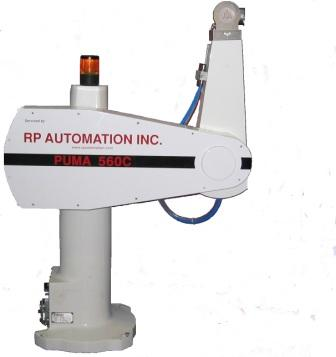
\includegraphics{images/Puma560.jpg}\\
\caption{The PUMA 560 robotic arm, which was the first to be used in surgery robotics in 1985}
\end{figure}
\end{center}

Some other important surgery robots are listed below:
\begin{itemize}
\item \textbf{AESOP\textsuperscript \textregistered Endoscope Positioner}
\item \textbf{HERMES\textsuperscript \textregistered Control Center}
\item \textbf{daVinci Surgical System\textsuperscript \textregistered}
\item \textbf{SOCRATES Robotic Telecollaboration System}
\item \textbf{Raven-II} \cite{Raven2}: An open platform for collaborative research on surgical robotics.
\end{itemize}

\begin{center}
\begin{figure}[H]
\centering
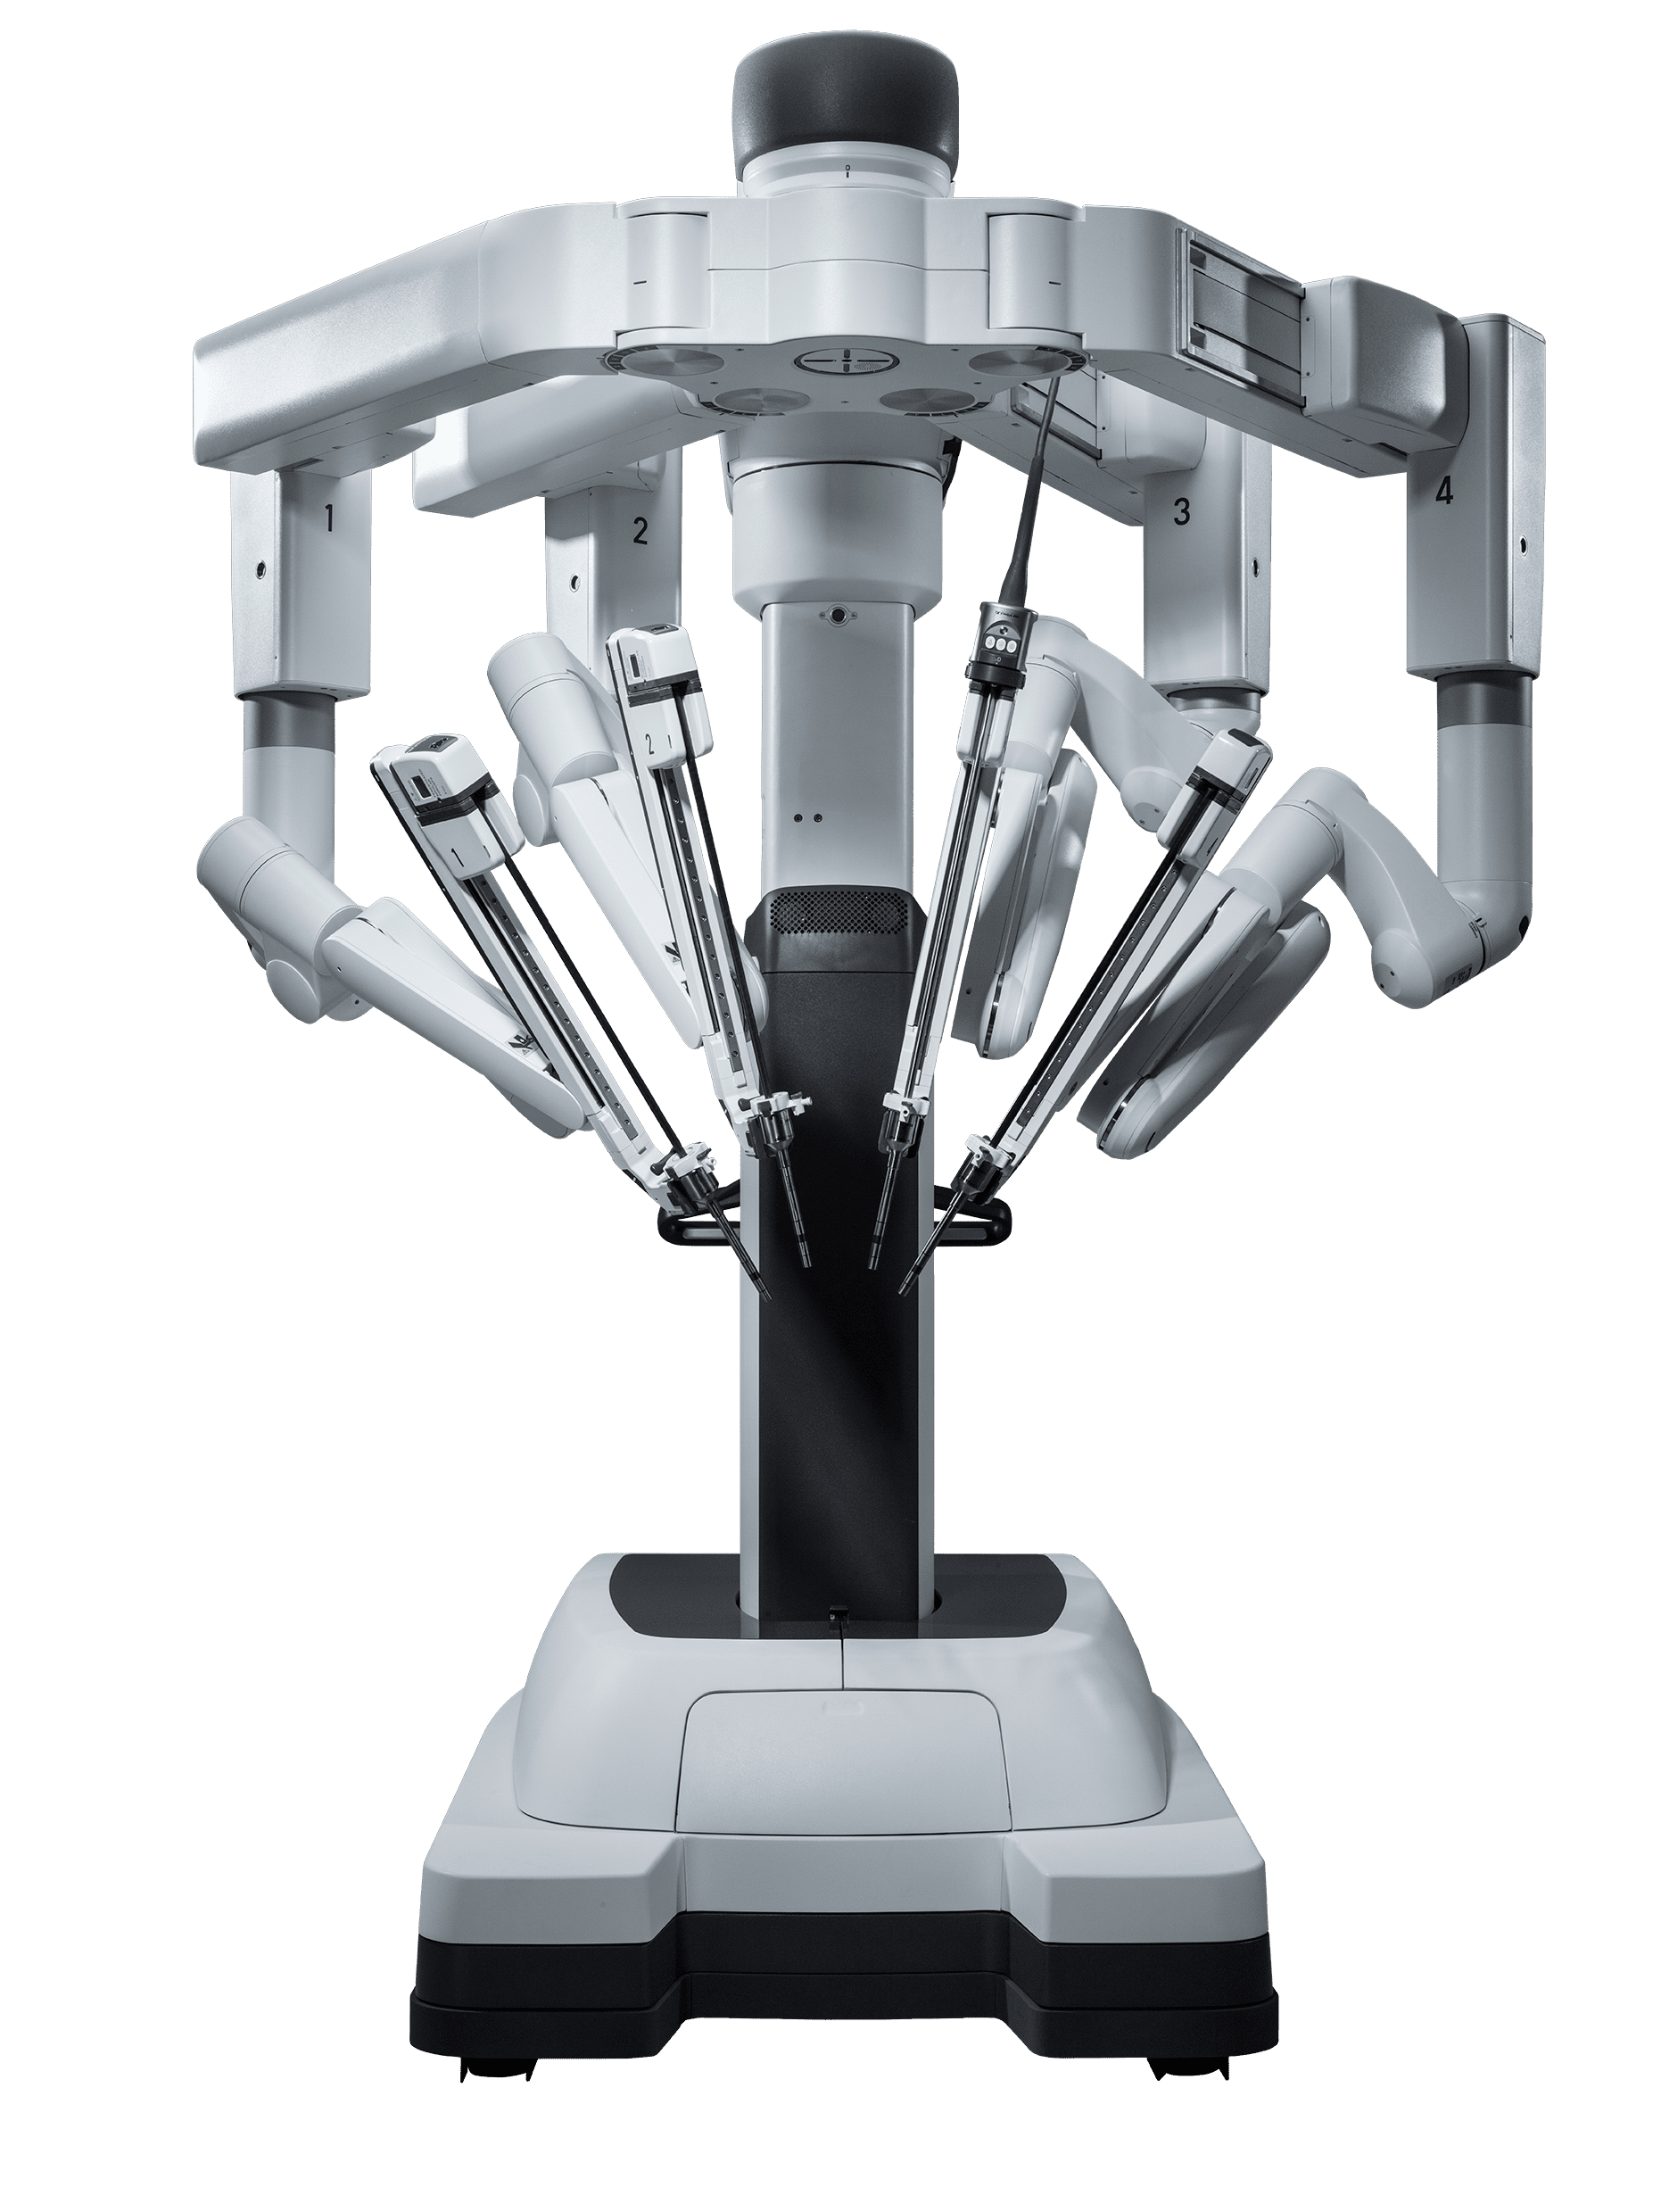
\includegraphics[width=9cm]{images/davinci-xi-patient-cart.png}\\
\caption{DaVinci Xi Patient Cart}
\end{figure}
\end{center}

Surgical robotics have a huge impact in Medicine and Healthcare in general. Some of the advantages are the following:
\begin{itemize}
\item \textbf{Minimally Invasive Procedures} which means
	\begin{itemize}
	\item Smaller incisions
	\item Less blood loss
	\item Reduced risk of inpatient infection
	\item Less pain
	\item Faster patient recovery
	\end{itemize}
\item Increased \textbf{precision} and reduced human errors
	\begin{itemize}
	\item Smooth and precise movements
	\item Detection and correction of errors caused by hand tremble
	\end{itemize}
\item \textbf{No fulcrum effect} and intuitive manipulation of surgical tools
\item \textbf{Haptic feedback}
\item \textbf{Teleoperation} (currently in the same room only): the surgeon operates while they sit on a special \textbf{ergonomic} console, which makes 
the long procedures more comfortable and efficient.
\end{itemize} 

\begin{center}
\begin{figure}[H]
\centering
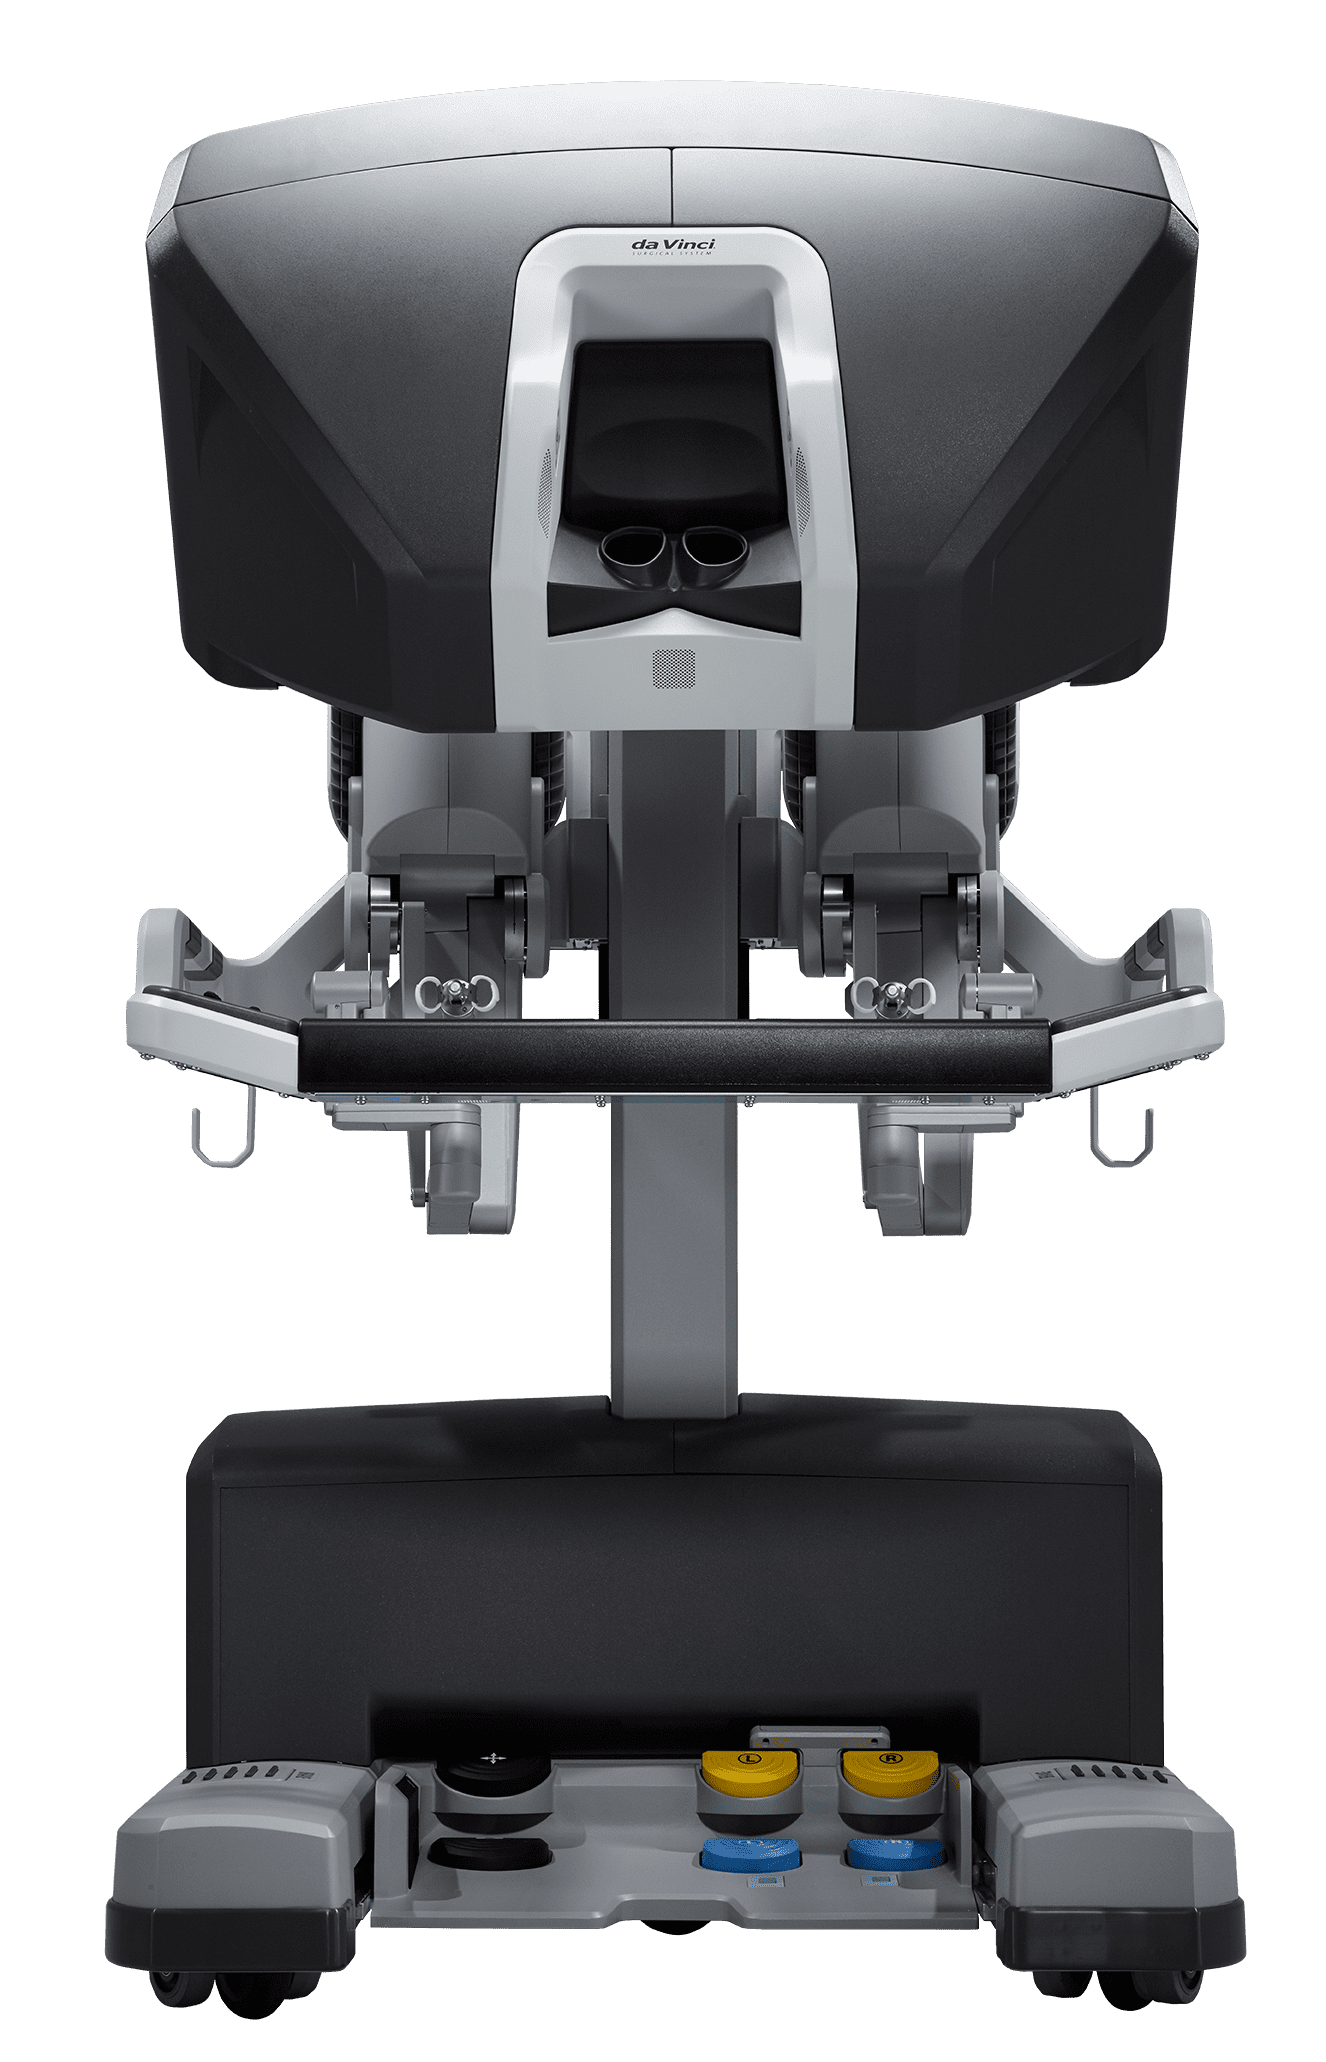
\includegraphics[width=7cm]{images/davinci-xi-surgeon-console.png}\\
\caption{DaVinci Xi Surgeon Console}
\end{figure}
\end{center}

\subsection{Bibliography Overview}

\subsection{Methodology \& Approach}
\section{Robotic arm Kinematic Analysis}


\subsection{Robotic arm, DH parameters \& Forward Kinematics}

\begin{center}
\begin{figure}[H]
\centering
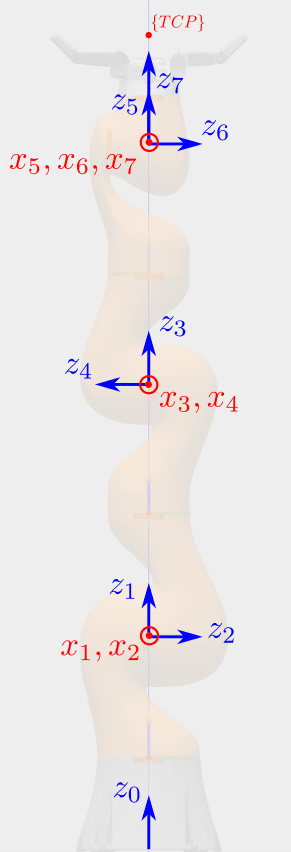
\includegraphics[height=12cm]{images/iiwa-frames.png}\\
\caption{Joint reference frames of the KUKA iiwa14 robot}
\end{figure}
\end{center}

\begin{center}
\begin{tabular}{ |c|c|c|c|c| } 
\hline
i & $θ_i$ (rad) & $L_{i-1}$ (m) & $d_i$ (m) & $α_{i-1}$ (rad) \\
\hline
1 & $θ_1$ & 0 & 0.36 & 0 \\
2 & $θ_2$ & 0 & 0 & $-π/2$ \\
3 & $θ_3$ & 0 & 0.36 & $π/2$ \\
4 & $θ_4$ & 0 & 0 & $π/2$\\
5 & $θ_5$ & 0 & 0.4 & $-π/2$ \\
6 & $θ_6$ & 0 & 0 & $-π/2$ \\
7 & $θ_7$ & 0 & 0 & $π/2$ \\
\hline
\end{tabular}
\end{center}

\[
^{i-1}T_i = 
\begin{bmatrix}
c\theta_i & -s\theta_i & 0 & L_{i-1} \\
s\theta_ica_{i-1} & c\theta_ica_{i-1} & -sa_{i-1} & -sa_{i-1}d_i \\
s\theta_isa_{i-1} & c\theta_isa_{i-1} & ca_{i-1} & ca_{i-1}d_i \\
0 & 0 & 0 & 1\\
\end{bmatrix}
\]


\subsection{Inverse Kinematics}

\subsubsection{Decoupling Technique}

In this section the inverse kinematics problem is solved for only the 6 out of the 7 total degrees of freedom. The third joint is not used in this 
analysis and it's angle is set to zero $θ_3 = 0$ . The rest of the joints form a special kind of kinematic chain that can be solved using the 
decoupling technique. In this technique the Inverse kinematics problem is split to 2 separate subproblems, one for the position and one for the 
orientation of the end-effector. This technique can be applied in this case because the axes of the 3 last joints intersect at the same point and 
they form an Euler wrist. \\

To solve for the joints' angles, the transformation matrix $^0T_7$ of the end-effector with respect to the robot's base is required. Usually the transformation ${}^UT_{tcp}$ is known, which is the pose of Tool's center point (TCP) with respect to the Universal Coordinate Frame $\lbrace U \rbrace$ from which the required $^0T_7$ can be calculated

\[
{}^UT_{tcp} = {}^UT_0  \;\;  {}^0T_7  \;\;   {}^7T_{tcp}
\]
\[
{}^0T_7 = {}^UT_0^{-1}  \;\;  {}^UT_{tcp}  \;\;  {}^7T_{tcp}^{-1}
\]
\[
{}^0T_7 = \begin{bmatrix}
R_t & \mathbf{p}_t \\
0 & 1 \\
\end{bmatrix}
\]

where ${}^UT_0,  \;\;   {}^7T_{tcp}$ are translation transformations by a constant distance and $R_t,  \;\; \mathbf{p}_t$ are the target's orientation 
and position respectively.

\[
{}^0\mathbf{p}_5 = {}^0T_4 {}^4\mathbf{p}_5 = \begin{bmatrix} p_x \\ p_y \\ p_z \\ \end{bmatrix}
\]

\begin{equation}
θ_1 = 
\begin{cases}
atan2 \left( p_y, p_x \right) \\
π - atan2 \left( p_y, p_x \right)
\end{cases}
\end{equation}

\begin{center}
\begin{figure}[H]
\centering
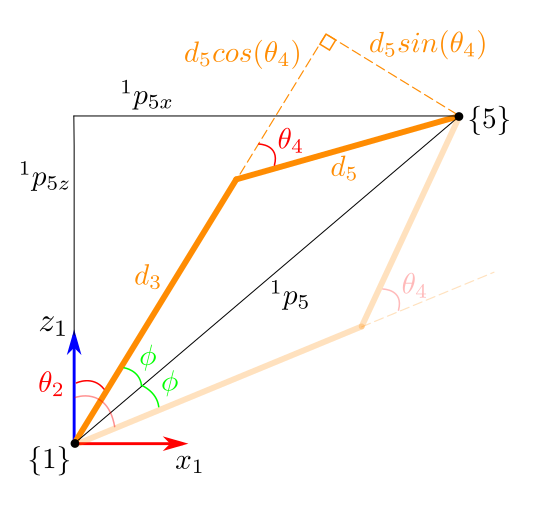
\includegraphics[width=8cm]{images/th2-4-calculation.png}\\
\caption{Calculation of angles $θ_2, θ_4$}
\end{figure}
\end{center}

\[
φ = acos \left( \frac{d_3^2 + \Vert{}^1p_{5}\Vert ^2 - d_5^2}{2d_3 \Vert{}^1p_{5}\Vert} \right)
\]
\begin{equation}
θ_2 = atan2 \left( \sqrt{p_x^2 + p_y^2}, {}^1p_{5z} \right) \pm φ
\end{equation}

\[ c_4 = \frac{ \Vert{}^1p_{5}\Vert ^2 - d_3^2 - d_5^2 }{2d_3d_5} \]
\begin{equation}
θ_4 = atan2 \left( \pm \sqrt{1 - c_4^2}, c_4 \right)
\end{equation}

Once $θ_1,θ_2,θ_3,θ_4$ are known, the orientation matrix of the wrist can be calculated as following
\[
R_{target} = 
\begin{bmatrix}
i_x & j_x & k_x\\
i_y & j_y & k_y\\
i_z & j_z & k_z\\
\end{bmatrix}
\]
\begin{equation}
θ_6 = atan2 \left( \pm \sqrt{1-k_y^2}, k_y \right)
\end{equation}
\[
θ_7 = atan2 \left( -j_y, i_y \right)
\]
\[
θ_5 = atan2 \left( - k_z, k_x \right)
\]


\subsubsection{Workspace constraints \& Singularity points}

\begin{center}
\begin{figure}[H]
\centering
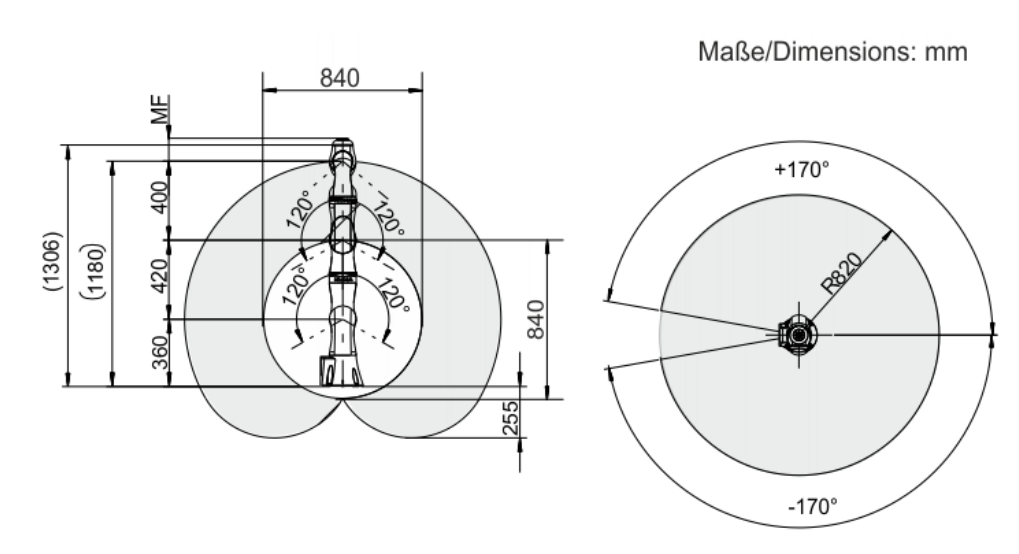
\includegraphics[width=10cm]{images/iiwa-workspace.png}\\
\caption{KUKA iiwa LBR14 workspace dimensions}
\end{figure}
\end{center}

Singularity points:
\begin{itemize}
	\item When $p_x^2 + p_y^2 = 0$ then the end-effector lies on the z-axis and $θ_1$ is not defined
	\item When $sin\left( θ_6 \right) = 0$ then the angles $θ_5, θ_7$ are not defined
\end{itemize}

\subsubsection{Solutions for 7DoF numerically}

\subsubsection{Comparison of Inverse Kinematics Techniques}

\section{Grasping}

\subsection{Gripper \& Forward Kinematics}

\begin{center}
\begin{figure}[H]
\centering
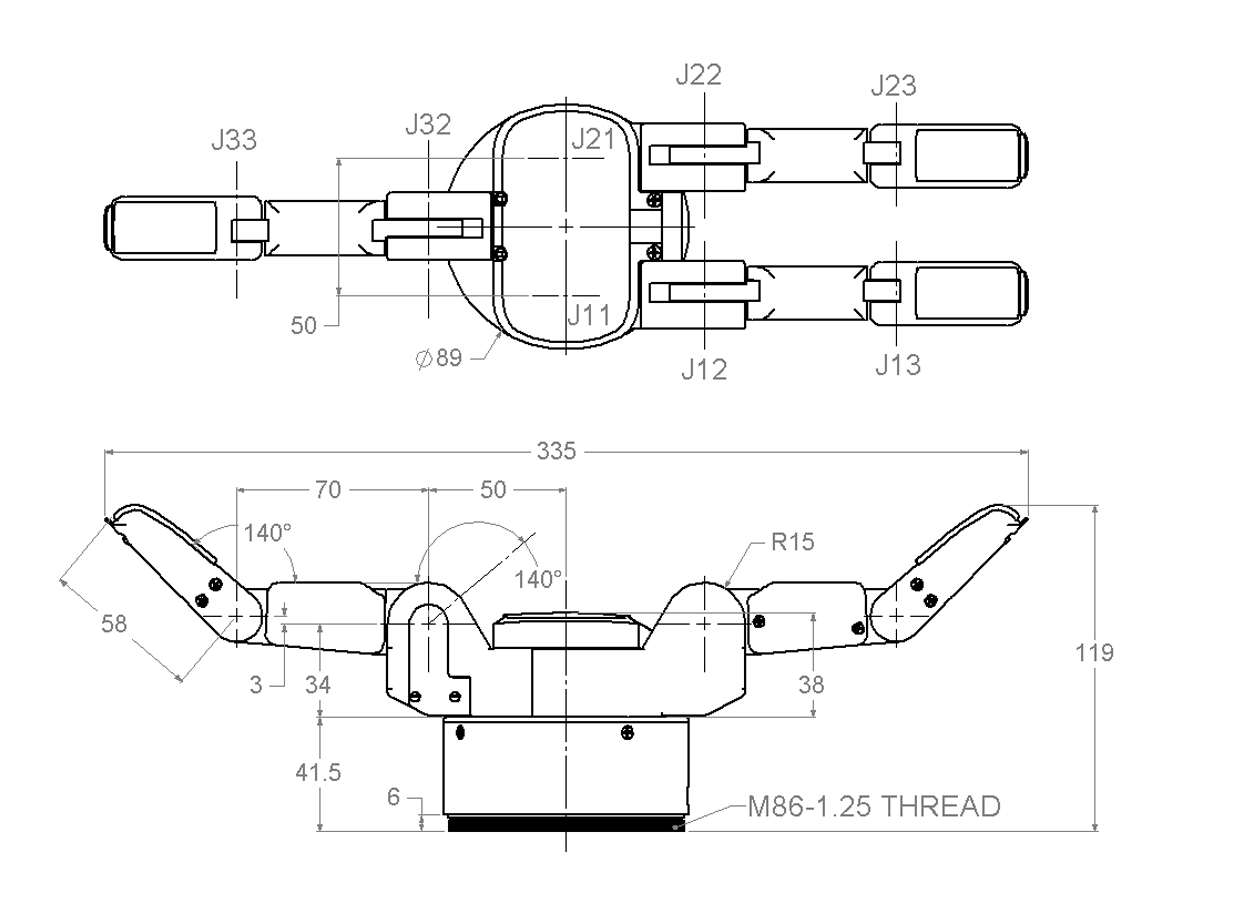
\includegraphics[width=12cm]{images/bh8-282-dimensions.png}\\
\caption{Barrett Hand gripper (model BH8-282) dimensions}
\end{figure}
\end{center}


\subsection{Gripper Inverse Kinematics}

The following Inverse Kinematics analysis referes to one finger of the Barrett Hand gripper, which has 3 revolute joints. Finger 3 has only 2 
revolute joints for which the angle solutions are the same with the solutions of the last 2 joints of the other fingers. Let

\[
\mathbf{p} = \begin{bmatrix} p_x \\ p_y \\ p_z \\ \end{bmatrix}
\]

be the position of the grasp point for one finger. The first angle can easily be calculated as

\begin{equation}
φ_1 = atan2 \left( p_y, p_x \right)
\end{equation}

Next, we calculate the third angle based on the law of cosines (see fig.)
\[
cos \left( π - φ_3 - \frac{π}{4} \right) = \frac{L_2^2 + L_3^2 - p^2}{2 L_2 L_3}
\]
\[
cos \left(φ_3 + \frac{π}{4} \right) = \frac{p^2 - L_2^2 - L_3^2}{2 L_2 L_3}
\]
\begin{equation}
φ_3 = atan2 \left[ \pm \sqrt{1 - \left( \frac{p^2 - L_2^2 - L_3^2}{2 L_2 L_3} \right)^2} , \frac{p^2 - L_2^2 - L_3^2}{2 L_2 L_3} \right] - \frac{π}{4}
\end{equation}

In a more general case, the first argument of the $atan2$ function in the expression of $φ_3$ could also be negative,
but in this case this second solution is rejected, because due to mechanical constraints, this angle can't be negative. 
After having calculated $φ_3$ we can calculate $φ_2 $

\[
tan \left( ψ + φ_2 \right) = \frac{p_z}{\sqrt{p_x^2 + p_y^2}}
\]
\[
tan \left( ψ \right) = \frac{L_3 sin \left( φ_3 + \frac{π}{4} \right) }{L_2 + L_3 cos \left( φ_3 + \frac{π}{4} \right)}
\]

\begin{equation}
φ_2 = atan2 \left( pz, \sqrt{p_x^2 + p_y^2} \right) - atan2 \left[ L_3 sin \left( φ_3 + \frac{π}{4} \right), L_2 + L_3 cos \left( φ_3 + \frac{π}{4} \right) \right]
\end{equation}

\subsection{Force closure}
The planar case, the spatial case \& convex hull test.

\lstinputlisting[frame=single,basicstyle=\ttfamily\small\color{blue},caption=Example ROS message with collision/contact information between one finger of the gripper and one surgical tool]{data/collision-contact-ros-message-example1.txt}
\section{Scene and object recognition with Computer Vision and Visual Servoing}

At this section we explore ways to detect and recognize the surgical tools as well as other objects of the simulation scene. To reduce the complexity of 
this thesis and focus on the more important features of this thesis, we assume in the simulation that the surgical tools are blue and the mounting dock, 
where the tools will be placed, is green. These assumptions make the scene and object recognition much easier without the need of more advanced image 
processing and/or machine learning recognition algorithms.\\

\textbf{Camera setup} used in this thesis:
\begin{itemize}
\item 2 HD RGB cameras with resolution $1280 \times 720$
\item near clipping plane: 0.02
\item far clipping plane: 300 
\item horizontal FoV (field of view): 1.396
\item update rate: 30fps
\end{itemize}

\subsection{Laparoscopic tool detection}

In order to detect the shape of the tool there are some standard steps that need to be executed. After having loaded the input image we convert it to grayscale, so that we can work on only one channel instead of
3 color channels and thus reduce the amount of calculations. Also for the purposes of extracting the shape of an object, the color doesn't have a very significant role in the algorithm. Next step is 
to remove the unwanted noise. In this thesis we only assume that the video frames have only Additive White Gaussian Noise (AWGN). To remove some of the
noise we use a moving average filter (the filter is also known as a kernel), which is convoluted around the whole image. The filter that was used is the following 3-by-3 matrix
\[
h = \frac{1}{9} \begin{bmatrix}
1 & 1 & 1 \\
1 & 1 & 1 \\
1 & 1 & 1 \\
\end{bmatrix}
\]
the output, filtered image is the result of the convolution of the image with the filter and is calculated as following
\[
g(i,j) = \sum_{k,l} f(i+k,j+l)h(k,l)
\]
where $g(\cdot, \cdot)$ is the output image and $f(\cdot, \cdot)$ is the input image.

After the noise is removed the image is getting binarized. To do that, we set a threshold, below which the pixels will be black and the rest will be white. This conversion to binary format, makes it 
easier to extract the boundaries of the black shapes, which will correspnd to the boundaries of the objects of the initial image.

\begin{center}
\begin{figure}[H]
\centering
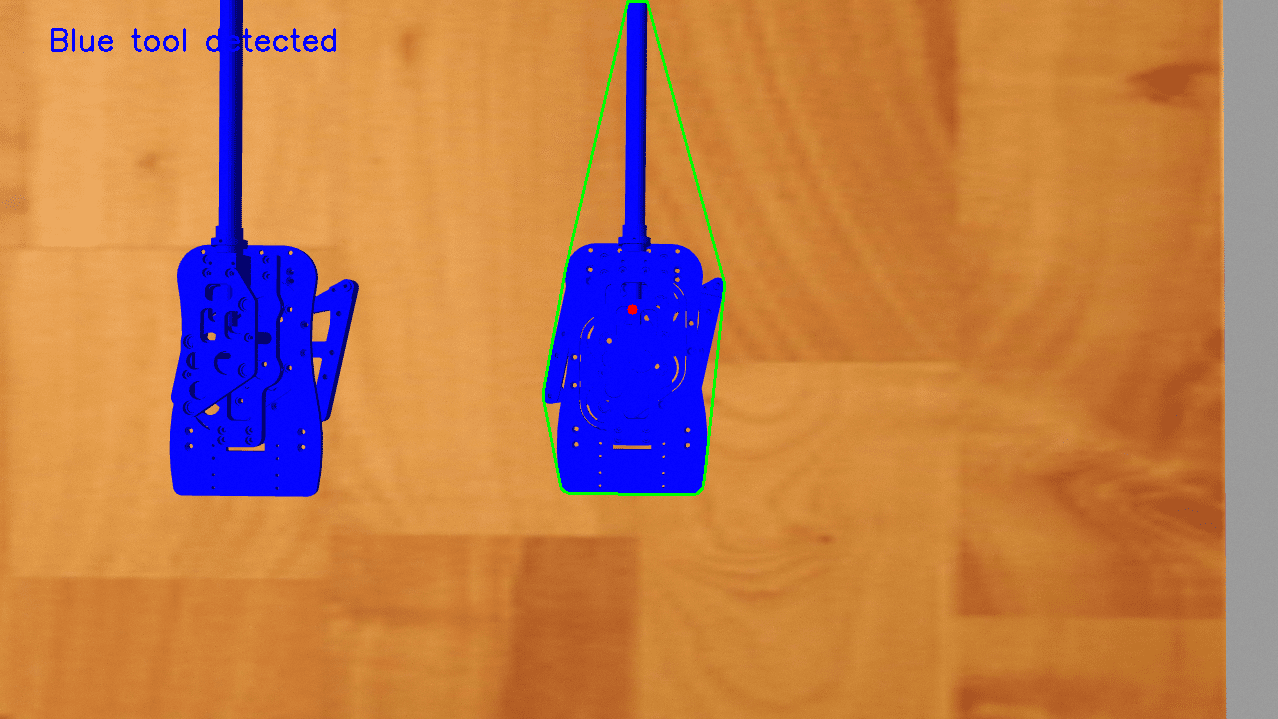
\includegraphics[width=12cm]{images/opencv-tool-convex-hull.png}\\
\caption{Simple tool detection in simulation based on color, using OpenCV. The green polygon is the convex hull, and the red point is the
estimated center of mass}
\end{figure}
\end{center}

\subsection{Stereoscopic vision}

\begin{center}
\begin{figure}[H]
\centering
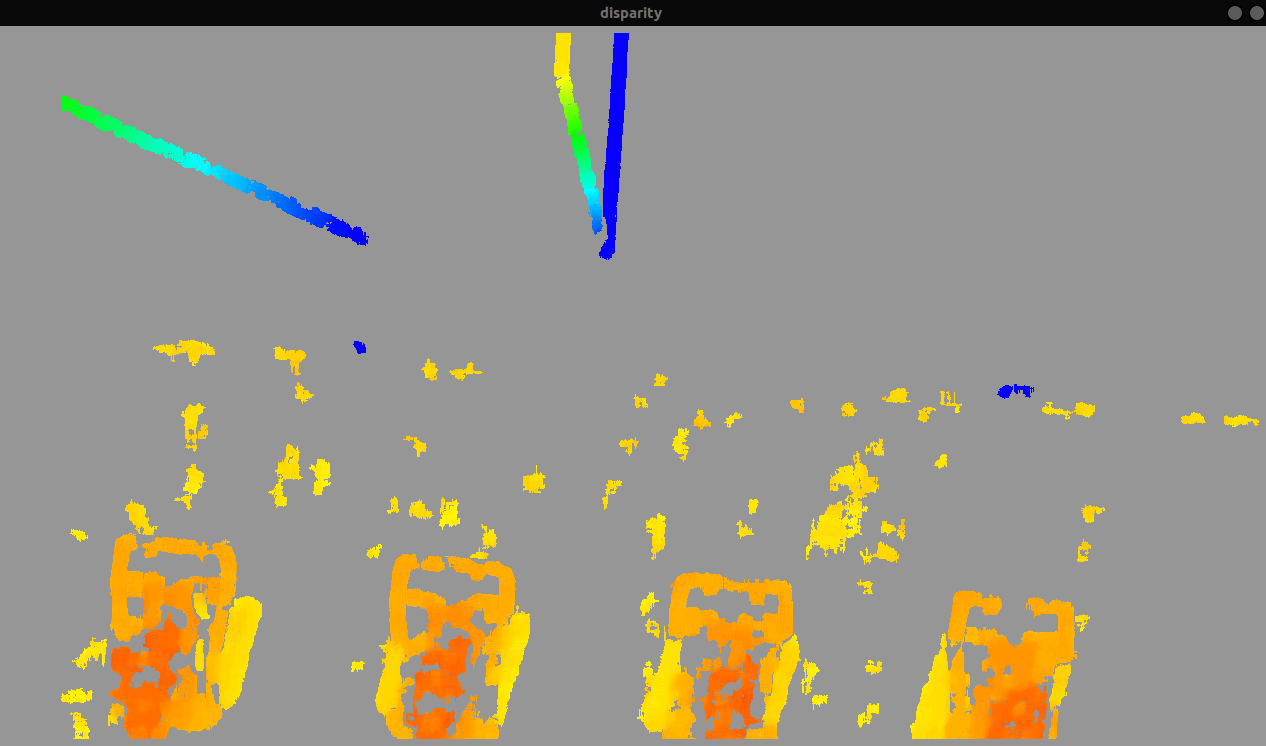
\includegraphics[width=12cm]{images/disparity.png}\\
\caption{Disparity image calculated from the 2 cameras}
\end{figure}
\end{center}

\begin{center}
\begin{figure}[H]
\centering
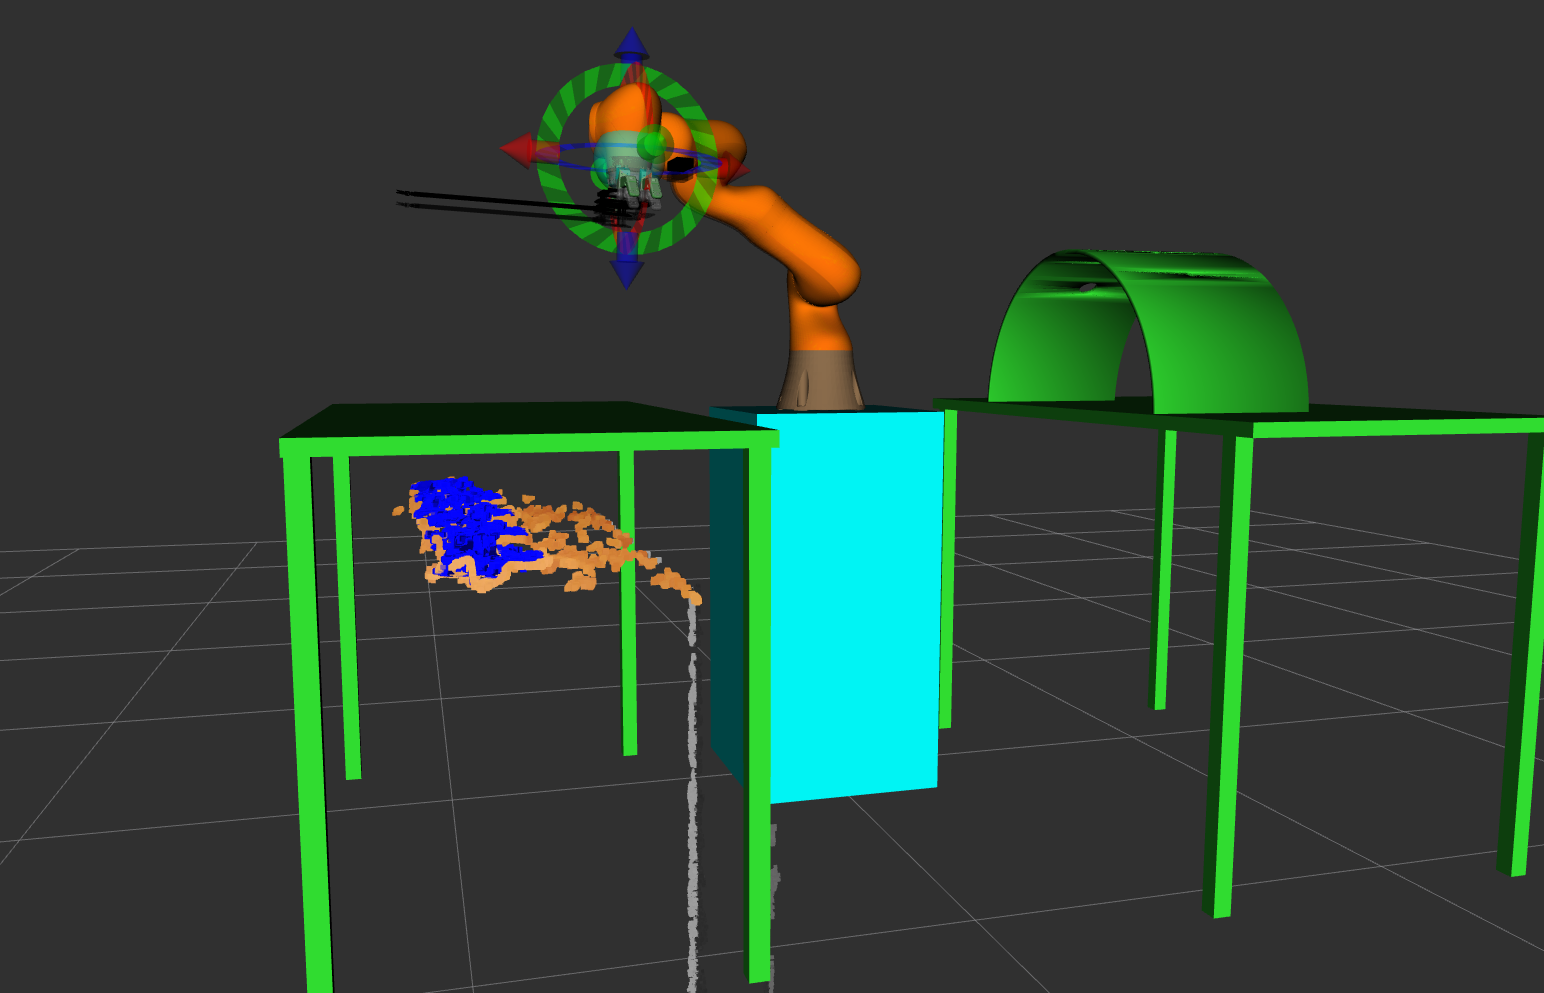
\includegraphics[width=12cm]{images/point_cloud.png}\\
\caption{Point cloud of surgical tools, generated from the 2 cameras and visualized in RViz}
\end{figure}
\end{center}

\subsection{Calculation of tool position and orientation}

In order for the gripper to grasp correctly the laparoscopic tool, it is required to calculate the tool's position and orientation in the pixel space 
which must then be converted with respect to the robot's workspace. From all the pixels that have been classified as part of the laparoscopic tool, 
one can estimate the center of mass and two perpendicular vectors 
attached to that point that define the orientation. The center of mass is simply the average of the $(x,y)$ coordinates of all the tool's pixels
\[
\left( \bar{x}, \bar{y} \right) = \left( \frac{1}{N}\sum_{i=1}^{N} x_i , \frac{1}{N}\sum_{i=1}^{N} y_i \right)
\]

The easiest way to calculate the center of mass is by calculating the average using the first moments of the contour points. However, since the contour is only using
the boundary of the object and not it's area, this method is not very accurate. To get a more accurate value for the center of mass, one must use the pixels that are inside 
the detected object's contour. The simplest way (but most expensive) to get the inside pixels of the tool is to loop over all the pixels and for each pixel check if it is inside the 
polygon (point inside polygon test). To make this method even faster, one can take a sample of the total pixels, for example check one in every 10 pixels in the x and y coordinates, 
which means reducing the time complexity to one tenth. \\

Taking this approach a step further in optimization, one can iterate not in all the video frame pixels but only those pixels 
that are inside the \textbf{Region of Interest} of the tool. The Region of Interest, also known as ROI, is a widely used structure in computer vision and is simply a bounding box (rectangle) that fits exactly 
(or is a bit bigger than) an object or part of the image frame that we want to study. Having already calculated the contour of the surgical tool and it's convex hull we can easily calculate this bounding box. 
For this calculation we prefer to use the convex hull, because it often contains much less pixels than the contour. We iterate over all the pixels of the convex hull and we get the minimum and maximum x and y 
coordinates. The combination of these four values is the desired ROI. Since we now have access to the tool's ROI, we can iterate and sample the pixels inside it (and not all pixels as we did before) to get 
some of the pixels of the tool so that we can more accurately calculate it's center of mass and orientation vectors. \\

The two orientation vectors are the eigenvectors of the covariance matrix of the above pixels. Let $\mathbf{a},\mathbf{b}$ be the orientation vectors, 
then $\mathbf{a},\mathbf{b}$ are solutions of the equation
\[
C \mathbf{v} = λ \mathbf{v}
\]
where $C$ is the covariance matrix given by
\[
C = \begin{bmatrix}
σ(x,x) & σ(x,y) \\
σ(y,x) & σ(y,y) \\
\end{bmatrix}
\]
\[
σ(x,y) = \frac{1}{n-1} \sum_{i=1}^{N} ( x_i - \bar{x} )( y_i - \bar{y} )
\]

\begin{center}
\begin{figure}[H]
\centering
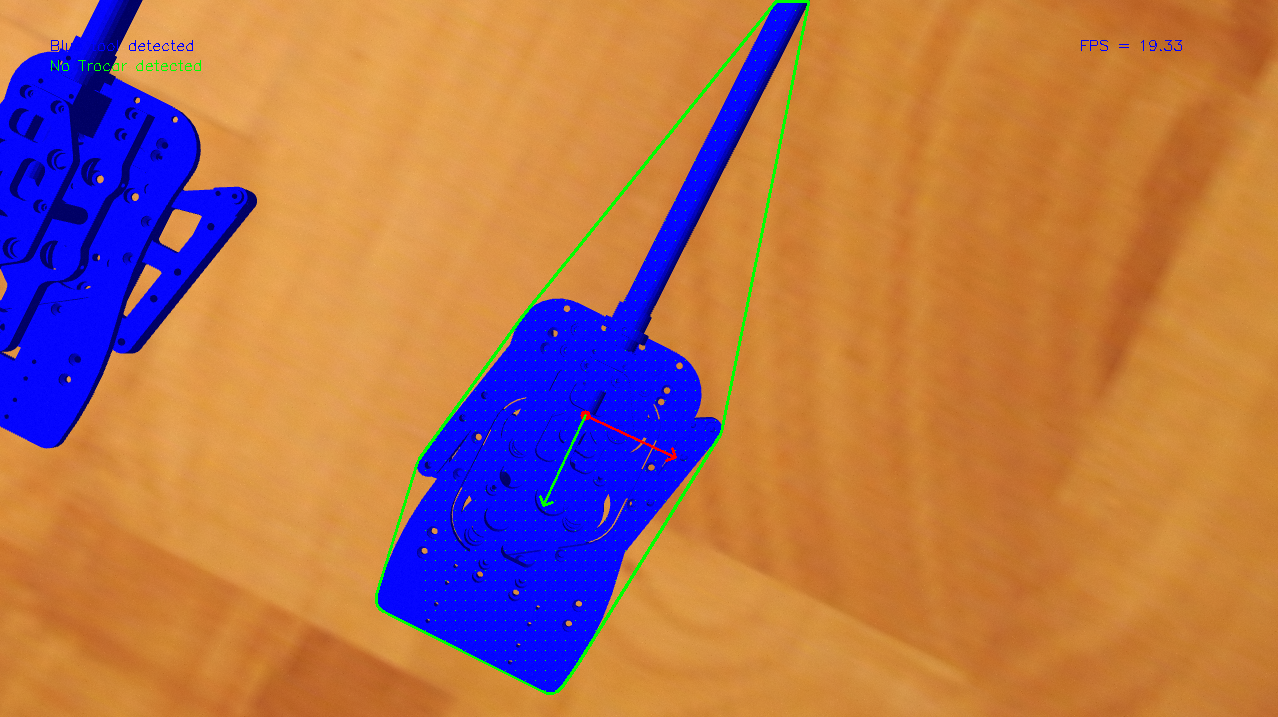
\includegraphics[width=0.8\textwidth]{images/tool-pose.png}\\
\caption{Estimation of tool's pose (position and orientation). The red dot is the center of mass and attached to that are the two orientation vectors of the tool. The green polygon is the convex hull of the tool 
and the white rectangle is it's ROI as calculated from the convex hull}
\end{figure}
\end{center}

\subsection{Calculation of grasping points}

\subsection{Trocar detection \& Estimation of fulcrum point}

\begin{center}
\begin{figure}[H]
\centering
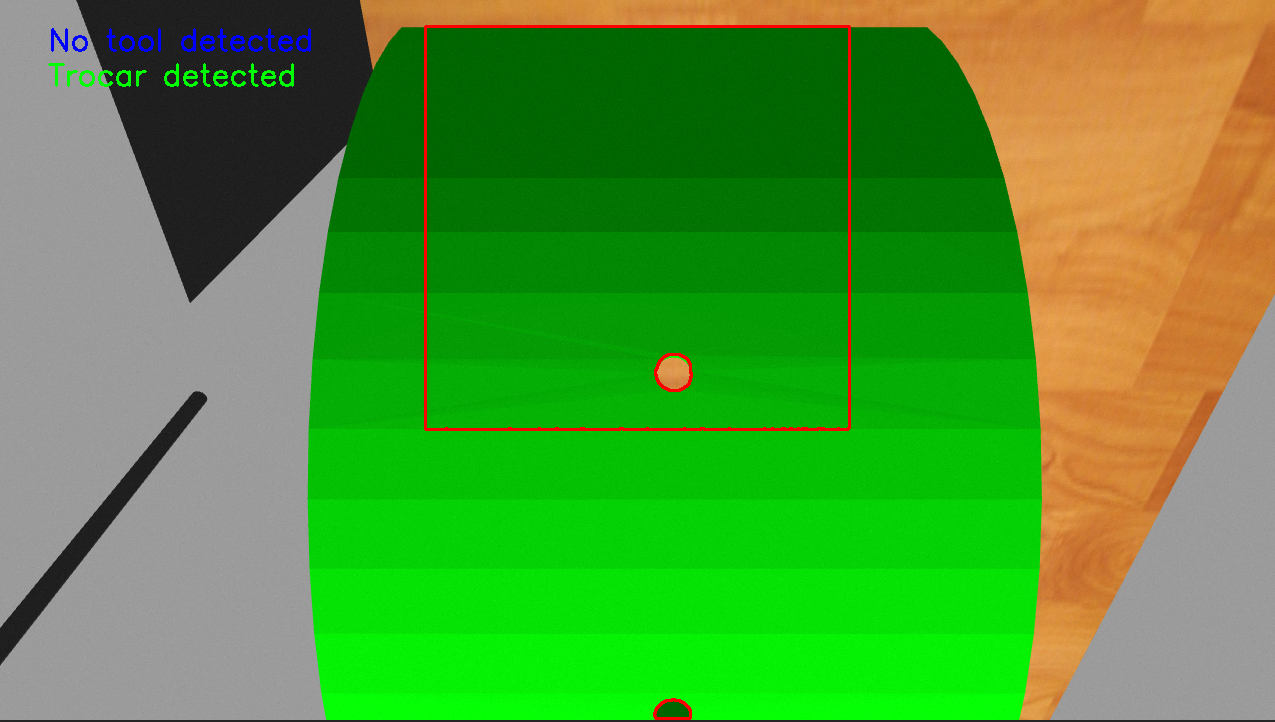
\includegraphics[width=12cm]{images/opencv-trocar-detection.png}\\
\caption{Simple trocar detection in simulation based on color, using OpenCV. In simulation, the trocar is simply considered to be a small 
cylindrical hole and it's center is the fulcrum point}
\end{figure}
\end{center}

\subsection{Visual Servoing}

At this chapter we briefly investigate how visual servoing can be applied in surgery robotics. \textbf{Visual Servoing} is the use of visual information 
to guide and control a robot. The main task of visual servoing is to control the end-effector's pose using features extracted from visual information. The 
features that are usually extracted from cameras are the position and orientation of the detected object, the distance of the object from the camera (using 
stereoscopic vision, photogrammetry or other techniques), the size and the shape of the object. The visual servoing can be executed either in the robot's space 
using position-based servoing or in the camera's space (also known as "pixel space") by using the image-based technique.

\subsubsection{Position based servoing}

\begin{center}
\begin{figure}[H]
\centering
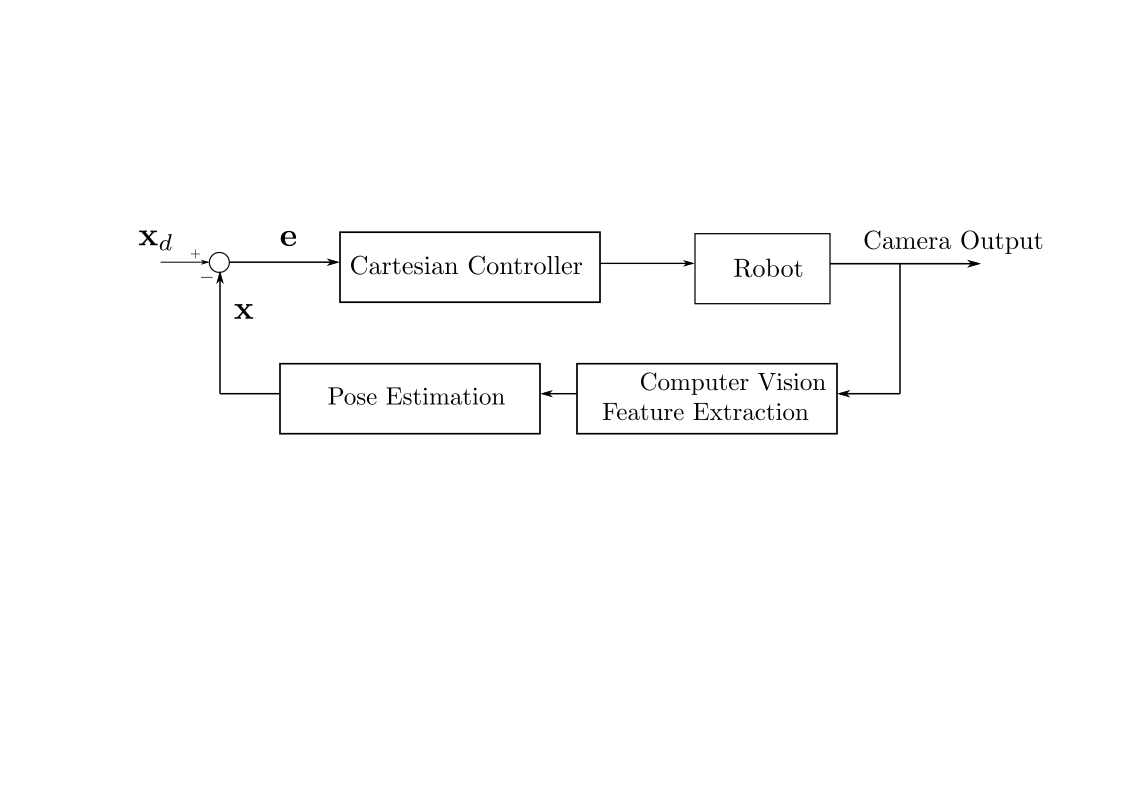
\includegraphics[width=0.8\textwidth]{images/visual-servoing-position-based.png}\\
\caption{Position based visual servoing closed loop control}
\end{figure}
\end{center}

\begin{itemize}
\item \textbf{Photogrammetric technique}
\item \textbf{Stereoscopic vision}
\item \textbf{Extracting depth from motion}
\end{itemize}

\subsubsection{Image based servoing}

\begin{center}
\begin{figure}[H]
\centering

\includegraphics[width=0.8\textwidth]{images/visual-servoing-image-based.png}\\
\caption{Image based visual servoing closed loop control}
\end{figure}
\end{center}

\begin{center}
\begin{figure}[H]
\centering
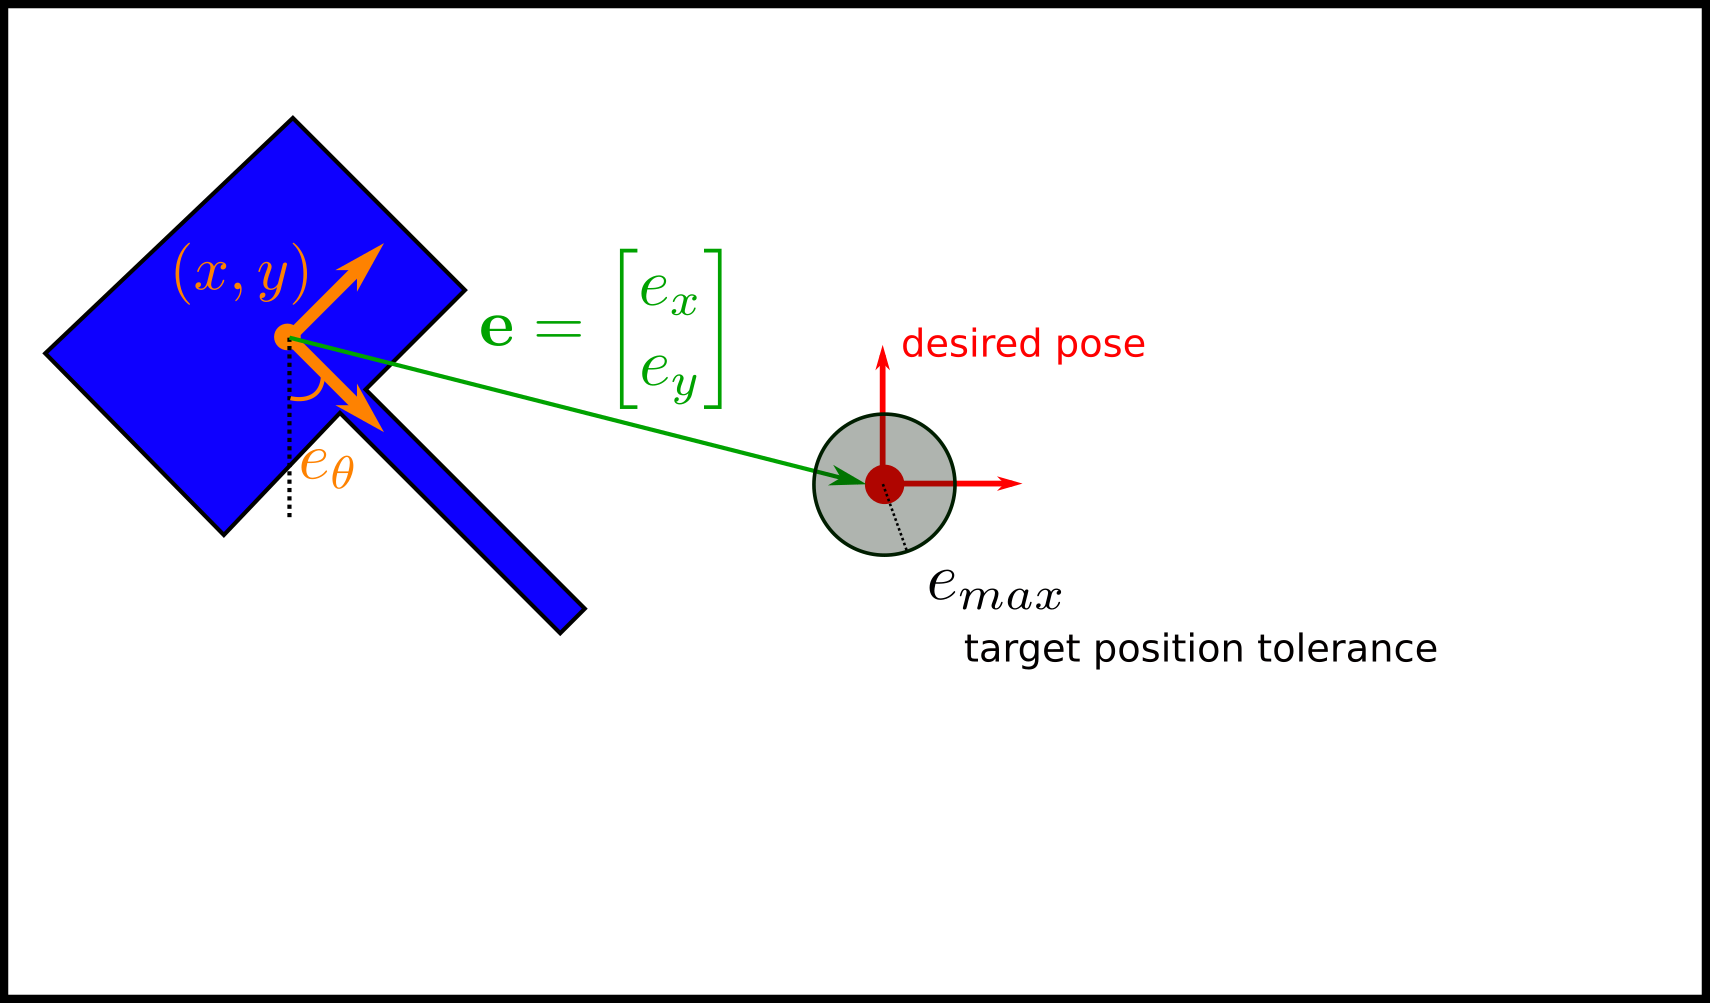
\includegraphics[width=0.45\textwidth]{images/visual_servo_start.png}
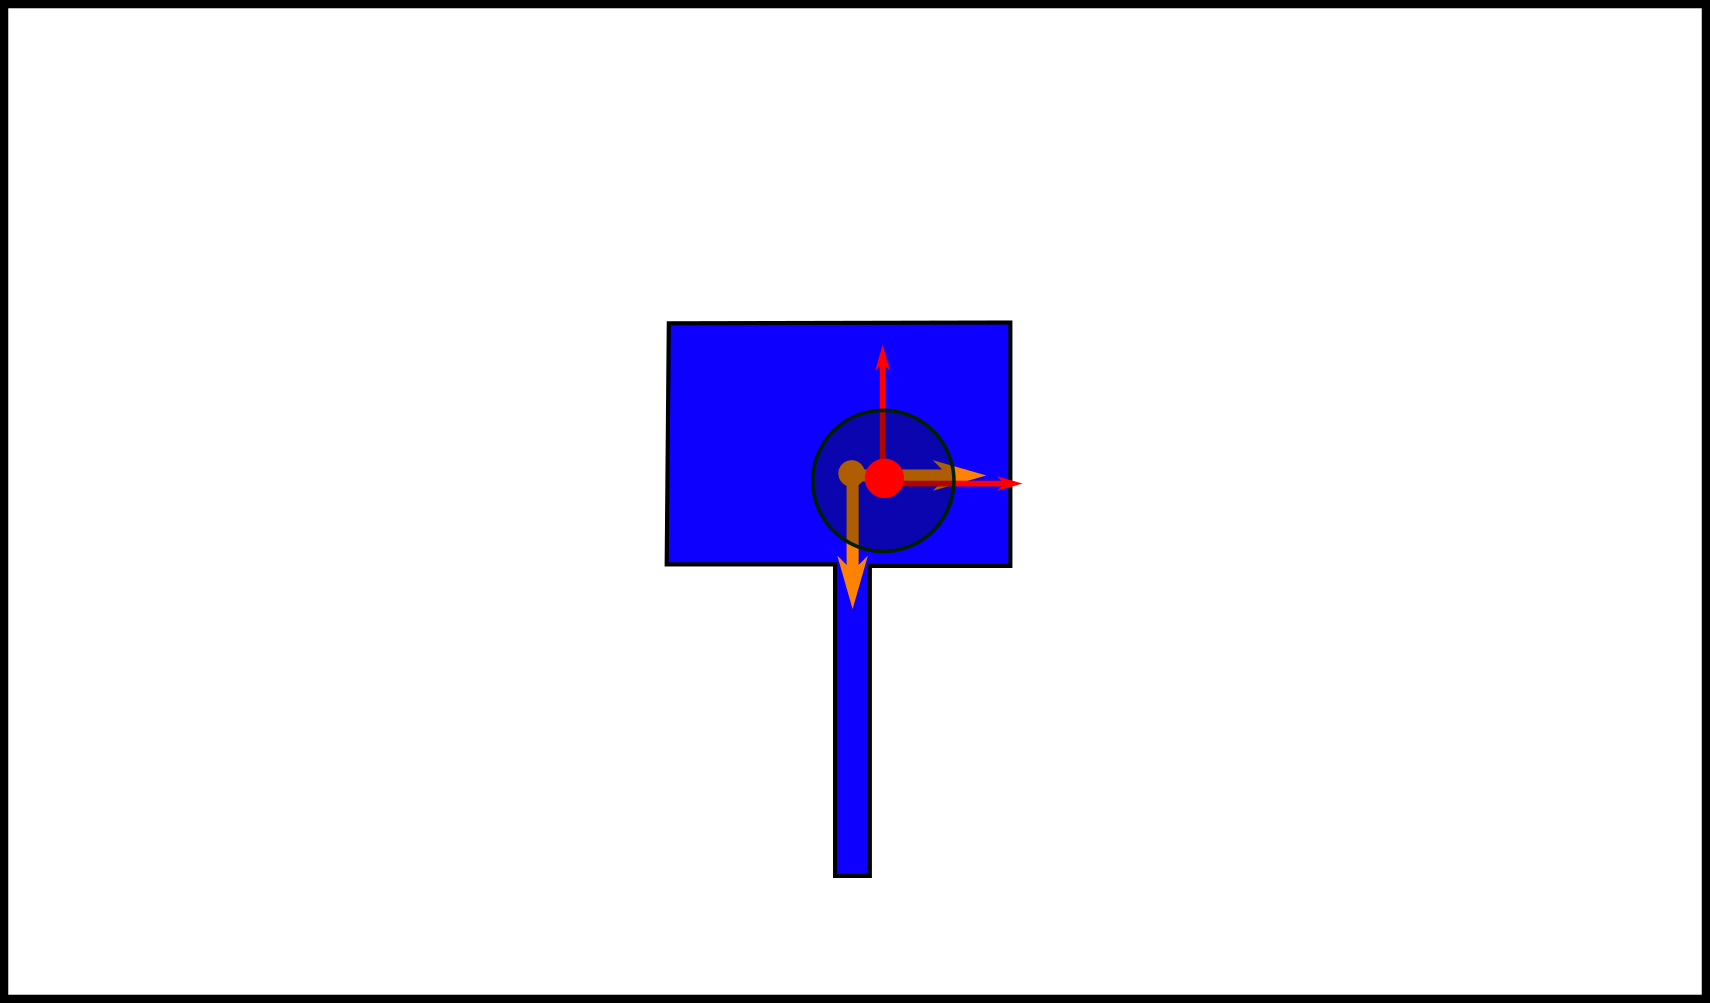
\includegraphics[width=0.45\textwidth]{images/visual_servo_end.png}\\
\caption{Image based visual servoing. The robot arm is controlled using the information gained from the video frames. The frames are 2Dimensional and thus 
the detected objects can have only 3 degrees of freedom which means we can mainly control 3 independent variables, here the $x,y,θ$ variables. The left image 
is the initial frame and the right image is the frame where the object is at the target pose.}
\end{figure}
\end{center}

\chapter{Path Planning}

\textbf{Path Planning} is a geometric problem, where it is desired to find a path from a starting point to a goal point and also satisfying a set of constraints, such as: 
restricting the solutions inside the robot's configuration space, avoiding obstacles in the task space, avoiding singularity points and respecting the robot's 
joint limits.


\section{Sampling methods}

The path planning algorithms that were mostly used in this thesis belong to the category of sampling methods. These methods use random functions to choose a sample from 
the configuration space or the state space. Sampling methods differ from the deterministic grid methods which, which discretize the whole space. Sampling methods are less 
computationally expensive than the grid methods, but they do not deliver optimal solutions like the latter.


\subsection{RRT Algorithms}

The \textbf{Rapidly-exploring Random Trees} algorithm is a sampling planning method that searches for an obstacle-free motion plan from an initial state $x_{init}$ to a set of goal states $\mathcal{X}_{goal}$. We refer to a set 
of goal states, because apart from the one desired goal state there can be other neighbor states that are within the allowed position and orientation tolerances.

\begin{algorithm}[H]
\SetAlgoLined
\ForEach{replanning attempt}{
	initialize vertices $V \leftarrow \lbrace x_{init} \rbrace$\;
	initialize edges $E \leftarrow \varnothing$\;
	initialize search tree $T \leftarrow (V,E)$\;
	\While{$time \leq maxPlanningTime$}{
		$x_{rand} \leftarrow$ getSampleStateFrom($\mathcal{X}$)\;
		$x_{nearest} \leftarrow$ getNearestNodeInTreeToState($T, x_{rand}$)\;
		$x_{new} \leftarrow$ findLocalPlanFromTo($x_{nearest}, x_{rand}$)\;
		\If{isPathCollisionFree($x_{nearest}, x_{rand}$)}{
			$V \leftarrow V \cup \lbrace x_{new} \rbrace $\;
			$E \leftarrow E \cup \lbrace (x_{nearest}, x_{rand}) \rbrace $\;
			\If{$x_{new} \in \mathcal{X}_{goal}$}{
				\Return SUCCESS and path plan $ T=(V,E) $ \;
			}
		}
	}
}
\Return FAILURE and $ T=(V,E) $ \;
\caption{RRT Algorithm}
\end{algorithm}

Other variations of the RRT Algorithm, which are also available in the OMPL library, included in the MoveIt library of ROS framework  are:
\begin{itemize}
	\item \textbf{TRRT} Transition-based RRT
	\item \textbf{BiTRRT} Bidirectional Transition-based RRT
	\item \textbf{RRT*}
	\item \textbf{RRTConnect} with is the default OMPL path planner in ROS
	\item \textbf{LBTRRT} Lower Bound Tree RRT
\end{itemize}


\subsection{PRM Algorithms}

The \textbf{Probabilistic Roadmap} (PRM) algorithm is a sampling planning method that constructs a roadmap representation of $\mathcal{C}_{free}$ \textbf{before searching} for a solution. After the roadmap is successfully built, then the algorithm searches 
for a solution using a traditional graph-based search algorithm. A very important aspect of this algorithm is how the sampling of the free configuration space will be done. The sampling is usually performed using a 
uniform distribution except from the regions close to objects where the sampling is more dense.

\begin{algorithm}[H]
\SetAlgoLined
initialize vertices $V \leftarrow \lbrace x_{init} \rbrace$\;
initialize edges $E \leftarrow \varnothing$\;
initialize roadmap graph $G \leftarrow (V,E)$\;
\For{$i = 1, \ldots , n$}{
	$x_{rand,i} \leftarrow$ getSampleStateFrom($\mathcal{X}$)\;
	$\mathcal{N}(x_{rand,i}) \leftarrow$ getKNearestNeighbors($G=(V,E), x_{rand,i}$)\;
	$V \leftarrow V \cup \lbrace x_{rand,i} \rbrace $\;
	\ForEach{$x \in \mathcal{N}(x_{rand,i})$}{
		\If{there is no edge between $x$ and $x_{rand,i}$}{
			\If{isPathCollisionFree($x_{nearest}, x_{rand,i}$)}{
				$E \leftarrow E \cup \lbrace (x_{rand,i}, x), (x, x_{rand,i}) \rbrace$
			}
		}
	}
}
\Return $G=(V,E)$
\caption{PRM roadmap construction (preprocessing phase)}
\end{algorithm}

Other variations of the PRM Algorithm, which are also available in the OMPL library, included in the MoveIt library of ROS framework  are:
\begin{itemize}
	\item \textbf{PRM*}
	\item \textbf{LazyPRM}
	\item \textbf{LazyPRM*}
\end{itemize}


\section{Pick and place algorithm}

% Help on using the algorithme package
% http://ftp.ntua.gr/mirror/ctan/macros/latex/contrib/algorithm2e/doc/algorithm2e.pdf 
\begin{algorithm}[H]
\SetAlgoLined
\ForEach{surgical tool}{
	\tcc{Plan the Pick pipeline}
	set grasp pose\;
	set pre-grasp approach\;
	set post-grasp retreat\;
	set posture of eef before grasp (open gripper)\;
	set posture of eef during grasp (closed gripper)\;
	\tcc{Plan the Place pipeline}
	set place location pose\;
	set pre-place approach\;
	set post-grasp retreat\;
	set posture of eef after placing object\;
	Plan pick and place paths\;
}
\caption{Pick and Place algorithm}
\end{algorithm}

If the pick and place algorithm targets small objects, such as cubes or spheres or other small convex objects then the path planning is straightforward. In the case where, the object to pick and place has at least one 
dimension that is bigger than the others like a rod or other long objects, such as the surgical tools, used in this thesis, then the path planning becomes more complicated, because of the almost certain collisions 
of the tool with the links of the rest of the robot (the link of the end-effector will probably not collide with the tool).


\section{Task space analysis}

Before designing any paths and trajectories it is very important to better understand the taskspace in which the surgical tool will operate in. When the robot arm is in the pick-and-place phase where it detexts the surgical 
tool and grasps and then go to the mounting dock to insert it, then at this phase, the taskspace is the same as the robot's taskspace. However, when the surgical tool is inserted in the patient's body and starts executing 
pivoting motions, then there are 2 taskspaces that are studied. The first one is the surgical taskspace, which is where the surgical movements are planned (sutures, laparoscopic camera movements etc.) and the second 
taskspace is the one outside of patient's body in which the planned paths are "mirrored" so that the robot can execute them. The surgical taspace $\mathbb{S}$ is the one shown in figure \ref{surgical-taskspace}. The paths inside 
the surgical task are transformed via the Fulcrum effect transformation, which is described in more detail in \ref{section:fulcrum-effect}, to the pivot paths taskspace $\mathbb{P}$ which is a subset of the robot's taskspace 
$\mathbb{T}$ (we assume that all pivot motions can be executed, i.e. that all motions are reachable and fully inside the robot's taskspace). The paths are then used as input to a trajectory generator whose output 
is transformed via the Inverse Kinematics equations to the joint angles that belong to the joint space $\mathbb{J}$. \\

Alternatively in a mathematical notation, the fulcrum effect transformation is notated as
\begin{equation}
Φ: \mathbb{S} \longrightarrow \mathbb{P}
\end{equation}
the inverse kinematics transformation is described as
\begin{equation}
IK: \mathbb{P} \subset \mathbb{T} \longrightarrow \mathbb{J}
\end{equation}
and similarly the forward kinematics transformation can be described as
\begin{equation}
FK: \mathbb{J} \longrightarrow \mathbb{T}
\end{equation}\\

\begin{center}
\begin{figure}[!htb]
\centering

\includegraphics[width=\textwidth]{images/spaces-and-transformations.png}\\
\caption{The spaces studied in this thesis and how they are connected with each other via transformations}
\label{surgical-taskspace}
\end{figure}
\end{center}

Having defined all the spaces, the Dexterity metric of the tool's task space (same as the surgical taskspace) can be defined as
\begin{equation}
\mathcal{D} = \mathcal{L}_q \mathcal{M}
\label{dexterity-measure}
\end{equation}
where
\begin{equation}
\mathcal{M} = \sqrt{det(J J^\top)}
\end{equation}
\begin{equation}
\label{joint-limit-measure}
\mathcal{L}_{q}=1-\exp\left\{-\kappa\prod_{i=1}^{n_{k}}\frac{(q_{ {i}}-q_{i,\min})(q_{i,\max}-q_{i})}{(q_{i,\max}-q_{i,\min})^{2}}\right\}
\end{equation}

\begin{center}
\begin{figure}[!htb]
\centering
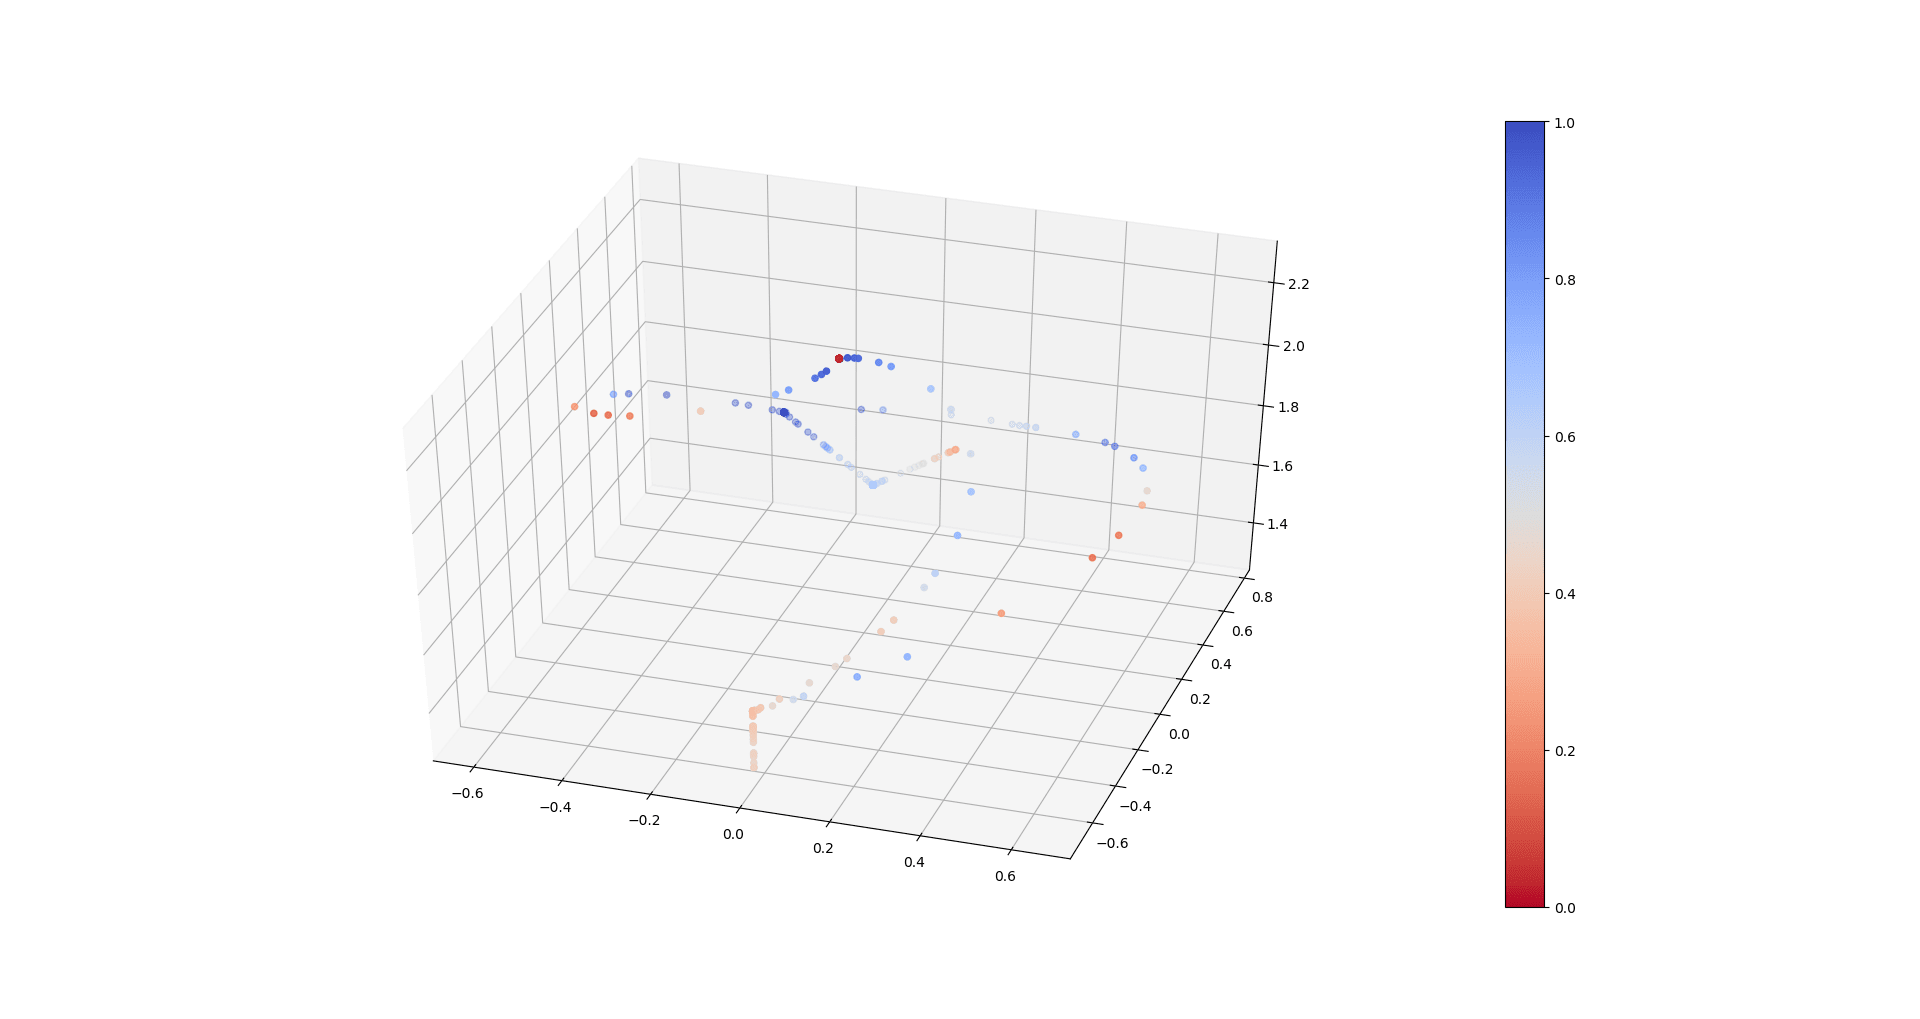
\includegraphics[width=10cm]{images/robot-planner1-manipulability-plot.png}\\
\caption{Plot the manipulability of the robot arm at sample points of the executed trajectory}
\end{figure}
\end{center}

The equation \ref{joint-limit-measure} calculates a joint limit measure which is multiplied with the manipulability measure and gives the dexterity measure.
From that equation we can conclude the following:
\begin{itemize}
\item If $q_i = q_{min}$ or $q_i = q_{max}$ then the exponential is equal to 1 which means that $\mathcal{L}_{q}$ and $\mathcal{D}$ are both 0, which means 
that the robot has \textbf{no dexterity at the boundary of the task space}.
\item If the value of $q_i$ is close to it's boundary value then the dexterity approaches 0. The how much close or far it is from the boundary (or in other words 
how fast the exponential term converges) depends on the parameter $\kappa$
\item The $q_{min}, q_{max}$ are calculated from the geometry of the task-space
\end{itemize}

For maximum dexterity at most points of a trajectory in a pivoting motion, the pivot sub-
taskspace (i.e. the space of all configurations of feasible pivot motions) must be fully within 
the robot’s whole reachable taskspace, otherwise only a small range of pivot movements will be 
feasible.\\

Finding $q_{i,min}, q_{i,max}$ at \ref{joint-limit-measure} is very difficult and time-consuming especially at task spaces with more intricate geometries. 
A similar and more practical equation to \ref{joint-limit-measure} can be written for calculating the dexterity of the robot in task space:

\begin{equation}
\label{rcm-taskspace-limit-measure}
\mathcal{L}_{p}=1-e^{-\kappa (r_{max} - r)}
\end{equation}
where $r_{max}$ is the maximum radius of a circle that the tool tip can follow at a given insertion depth $z$. Moreover, at every point of the taskspace, it is $L^2 = r^2 + z^2$. 
The equation \ref{rcm-taskspace-limit-measure} however only shows dexterity in terms of approaching the boundary of the taskspace and it does not take into consideration internal points of low 
dexterity and singularities like equation \ref{dexterity-measure}.

\begin{listing}[H]
\begin{minted}[tabsize=2,breaklines,frame=lines,framesep=2mm,baselinestretch=1.2,fontsize=\footnotesize, linenos]{matlab}
x = []; y = []; z = [];
r = [];
s = 0:0.005:0.5;
L = 0.48;
k = 4.5;

for z0=-L:0.01:0
    if abs(z0)*sqrt(2) <= L
        rmax = abs(z0);
    else
        rmax = sqrt(L^2-z0^2);
    end
    for r0=0:0.02:rmax
        x = [x, r0*cos(2*pi*s)];
        y = [y, r0*sin(2*pi*s)];
        z = [z, z0*ones(size(s))];
        lp = 1-exp(-k*(rmax-r0));
        r = [r, lp*ones(size(s))];
    end
end
\end{minted}
\caption{RCM Taskpace calculation using MATLAB}
\label{code:rcm_taskspace_matlab}
\end{listing}

\begin{center}
\begin{figure}[!htb]
\centering
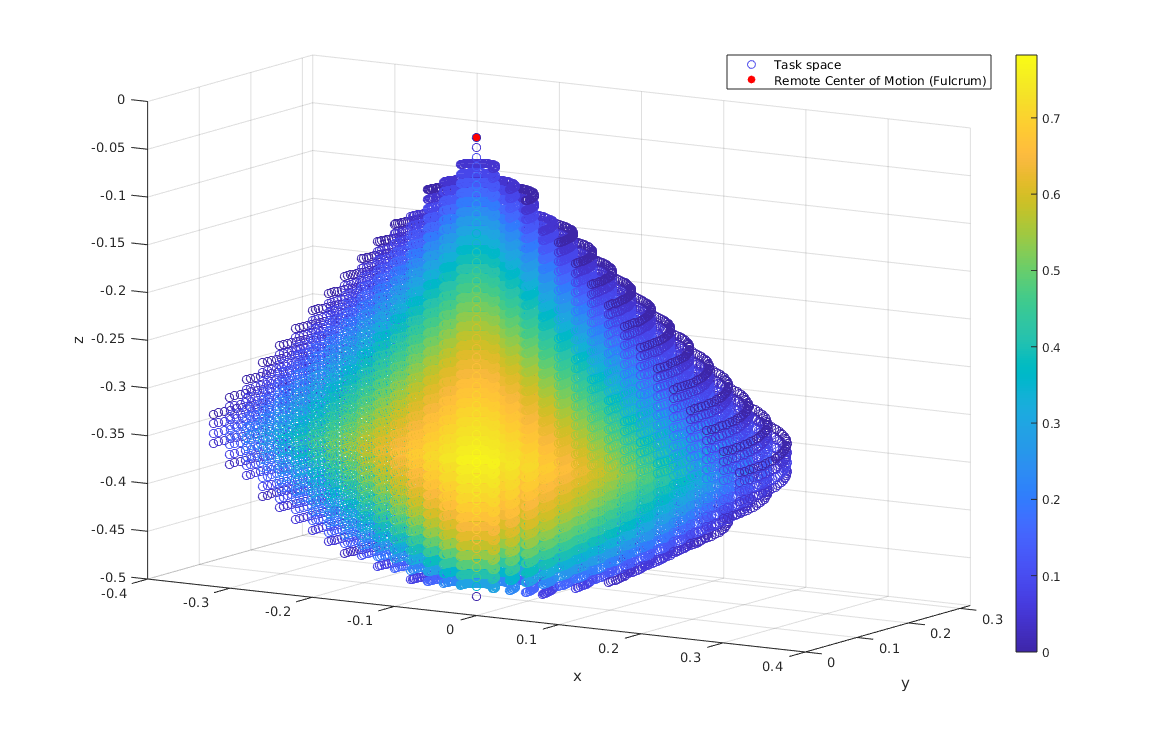
\includegraphics[width=0.8\textwidth]{images/rcm_taskspace.png}\\
\caption{Task space inside patients body. Colors with 0 or low value correspond to points with low dexterity. This is the trivial case, where no collision objects are taken into consideration}
\label{surgical-taskspace}
\end{figure}
\end{center}

All of the metrics above, measure how much reachable are various points of the surgical taskspace, but they are calculated from different perspectives, using input values from different spaces.
\begin{equation}
\mathcal{L}_{q}, \mathcal{M}: \mathbb{J} \longrightarrow \mathbb{R} \quad \textrm{and} \quad
\mathcal{L}_{p}: \mathbb{S} \longrightarrow \mathbb{R}
\end{equation}
\section{Trajectory Planning - Laparoscopic tool manipulation}

At this step, given the points of the desired path, a more detailed trajectory is calculated, 
which will contain all the waypoints that the robot will have to visit. Trajectory planning is executed after a desired path is generated,
and consists in mapping the geometric points to specific \textbf{time points}, as well as assigning specific \textbf{velocities}, \textbf{accelerations} and \textbf{jerks}, 
in order to generate the commands needed for the robot controller to execute a smooth motion.

The paths that are calculated are parameterized by the path parameter $s$. As $s$ increases from $0$, the robot moves from the start configuration $q(0)$ to the goal configuration $q(1)$. 
Path planning outputs geometric information $q(s), s \in [0, 1]$, whereas the \textbf{trajectories} that are the subject of this chapter, also include \textbf{time information} $q(t), t \in [0, T]$. 
A path can be converted to a trajectory by defining a function $s(t): [0, T] \rightarrow [0, 1]$ which maps the time parameter's range to the path parameter's range. This function is also known as \textbf{time scaling} or 
\textbf{time parameterization}.The most common methodology of trajectory planning, which is also used in this thesis, is the one that is studied in the \textbf{joint angles space} also known as \textbf{configuration space}.

The biggest challenge in manipulating a laparoscopic tool with a robot is overcoming the \textbf{fulcrum effect} problem. This is also one of the reasons that 
robotic assisted surgery replaced the traditional laparoscopic procedures. The fulcrum effect means that the surgeon's hand motions are inverted and scaled 
with respect to the Remote Center of Motion point, which lies approximately on the center of the incision. Apart from the scaling and inversion, laparoscopic 
procedures add an additional motion constraint that demands at each time one point of the laparoscopic tool to coincide with the RCM point.

\subsection{Tool pose}

\begin{center}
\begin{figure}[H]
\centering
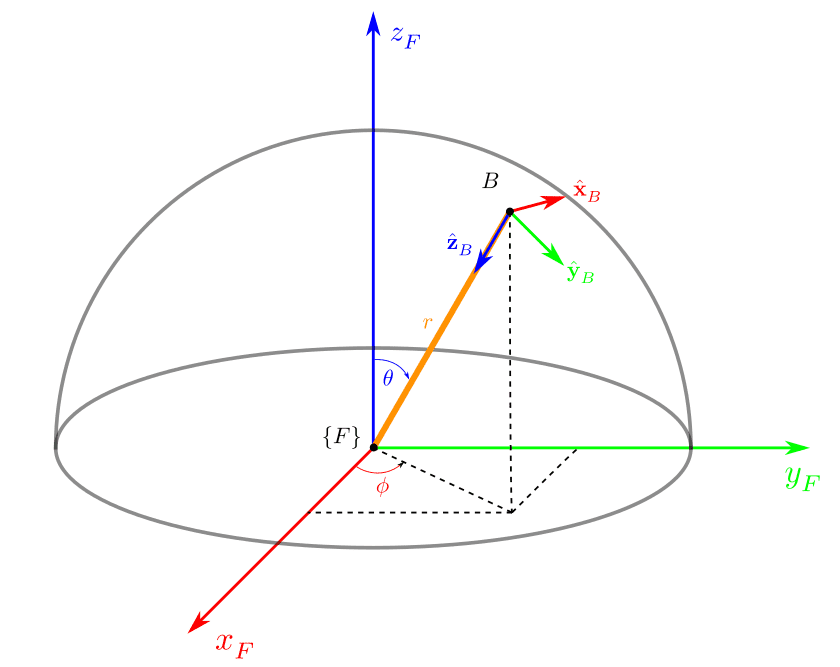
\includegraphics[width=12cm]{images/fulcrum-space.png}\\
\caption{Tool pose at target point $B$ calculated with respect to Fulcrum's reference frame $\lbrace F \rbrace$}
\end{figure}
\end{center}

The laparoscopic tool pose is given by the position and orientation vectors at target point $B$ with respect to the coordinate frame $\lbrace F \rbrace$.
The pose is given by the following transformation matrix
\[
{}^{F}T_B = \begin{bmatrix}
{}^{F}R_B & {}^{F}\mathbf{p}^{}_B \\
\mathbf{0} & 1 \\
\end{bmatrix}
\;\; where \;\;
{}^{F}R_B = \begin{bmatrix}
\hat{\mathbf{x}}^{}_B & \hat{\mathbf{y}}^{}_B & \hat{\mathbf{z}}^{}_B \\
\end{bmatrix}
\]

\begin{equation}
\hat{\mathbf{x}}^{}_B = \hat{\mathbf{θ}} = cos(θ)cos(φ)\hat{\mathbf{x}}^{}_F + cos(θ)sin(φ)\hat{\mathbf{y}}^{}_F - sin(θ)\hat{\mathbf{z}}^{}_F
= \begin{bmatrix}
cos(θ)cos(φ) \\
cos(θ)sin(φ) \\
- sin(θ) \\
\end{bmatrix}
\end{equation}

\begin{equation}
\hat{\mathbf{y}}^{}_B = \hat{\mathbf{φ}} = -sin(φ)\hat{\mathbf{x}}^{}_F + cos(φ)\hat{\mathbf{y}}^{}_F
= \begin{bmatrix}
-sin(φ) \\
cos(φ) \\
0 \\
\end{bmatrix}
\end{equation}

\begin{equation}
\hat{\mathbf{z}}^{}_B = - \hat{\mathbf{r}} = - (sin(θ)cos(φ)\hat{\mathbf{x}}^{}_F + sin(θ)sin(φ)\hat{\mathbf{y}}^{}_F + cos(θ)\hat{\mathbf{z}}^{}_F)
= \begin{bmatrix}
-sin(θ)cos(φ) \\
-sin(θ)sin(φ) \\
-cos(θ) \\
\end{bmatrix}
\end{equation}

The position of the point $B$ is given in spherical coordinates by:
\begin{itemize}
	\item $r=ρ$ : outside penetration of laparoscopic tool
	\item $θ=β$ : altitude angle
	\item $φ=α$ : orientation angle
\end{itemize}
thus the position with respect to the coordinate frame $\lbrace F \rbrace$ is given by
\begin{equation}
{}^{F}\mathbf{p}^{}_B = \begin{bmatrix}
ρsin(β)cos(α) \\
ρsin(β)sin(α) \\
ρcos(β) \\
\end{bmatrix} = ρ \hat{\mathbf{r}}
\end{equation}

The above goal point must be the same as the $TCP$ point of the robot's end-effector. This means, that this pose must be converted with respect to the robot's reference frames.
\[
{}^{U}T^{}_{TCP} = {}^{U}T^{}_{B}
\]
\[
{}^{U}T^{}_{0} \; {}^{0}T^{}_{7} \; {}^{7}T^{}_{TCP} = {}^{U}T^{}_{F} \; {}^{F}T^{}_{B}
\]
\begin{equation}
{}^{0}T^{}_{7} = {}^{U}T^{-1}_{0} \; {}^{U}T^{}_{F} \; {}^{F}T^{}_{B} \; {}^{7}T^{-1}_{TCP}
\end{equation}


\subsection{Trajectory planning in cartesian coordinates}
\label{subsection:pivot-motions}

On this section, some basic pivoting trajectories around the fulcrum point, are presented. In all of the following three example pivoting motions, we have made 
the assumption that the position and orientation of the ${F}$ reference frame is precisely known, which is however not applicable in real-life scenarios ()

\subsubsection{Circular trajectory of tool tip}

\begin{center}
\begin{figure}[H]
\centering
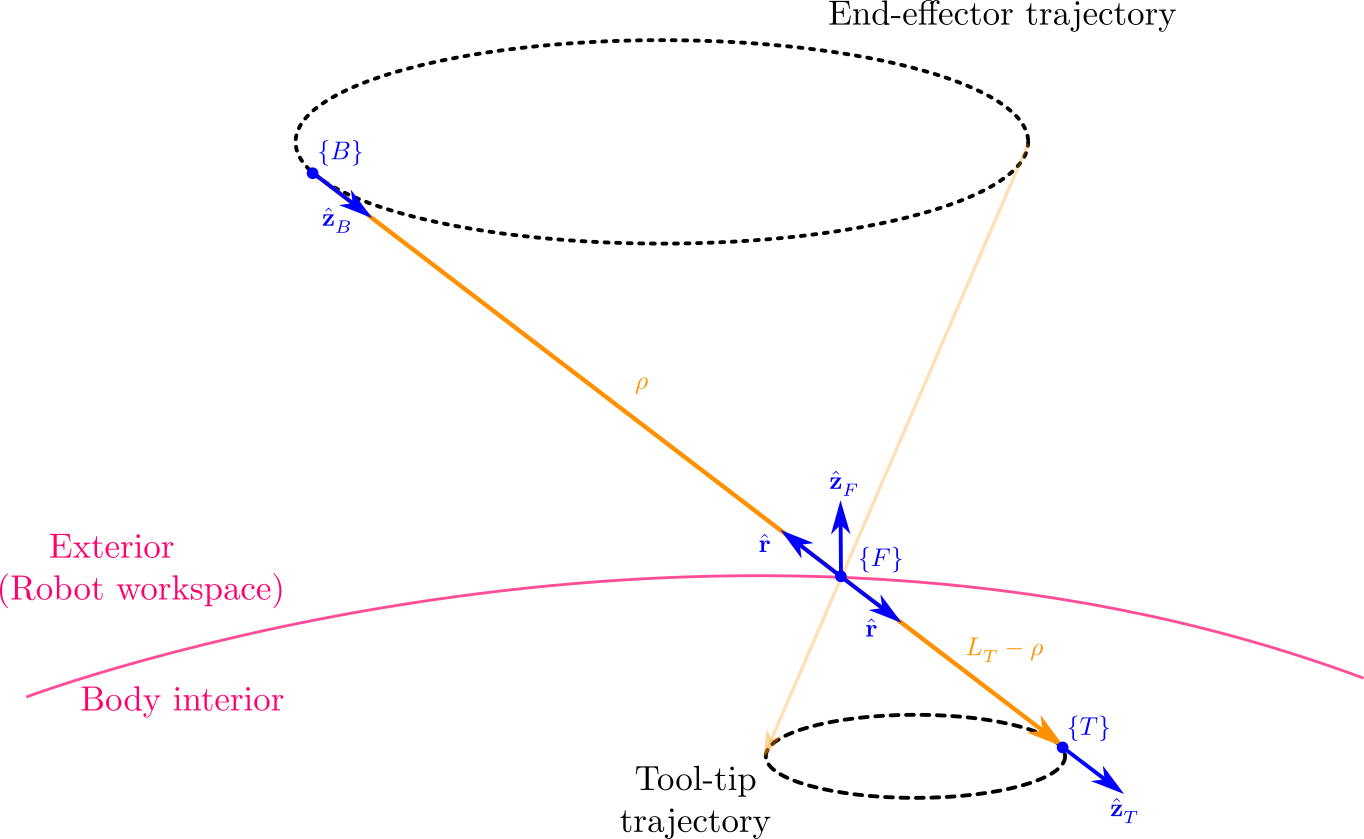
\includegraphics[width=12cm]{images/circular-trajectory-wrt-fulcrum.png}\\
\caption{Circular trajectory of tool tip with respect to Fulcrum reference frame}
\end{figure}
\end{center}

To generate a circular trajectory for the pivot movement we must specify the center of the circle 
and a vector whose magnitude is the radius of the circle and it’s direction gives the orientation 
of the plane that the circle lies at. The simplest case of a circular trajectory is the one, 
whose circle lies in a plane parallel to the xy plane.


We first consider the motion of the laparoscopic tool tip on a circle parallel to a z-plane, with respect to the $\lbrace F \rbrace$ coordinate frame.
\begin{equation}
(x^{}_{F} - x^{}_{F0})^2 + (y^{}_{F} - y^{}_{F0})^2 = r_0^2, \;\; z^{}_{F} = z^{}_{F0}
\end{equation}
It's often more convenient to express trajectories in a parametric form, which makes it easier to calculate all the waypoints of the trajectory
\begin{equation}
\begin{cases}
x^{}_{F} = r_0cos(2πs) + x^{}_{F0} \\
y^{}_{F} = r_0sin(2πs) + y^{}_{F0} \\
z^{}_{F} = z^{}_{F0}
\end{cases} ,
\;\;
s \in [0, 1]
\end{equation}

After having calculated the cartesian coordinates we can calculate the spherical coordinates as follows

\begin{equation}
\label{eqns:cartesian-to-spherical}
\begin{cases}
r = \sqrt{x^{2}_{F} + y^{2}_{F} + z^{2}_{F}} \\
θ = atan2 \left( \sqrt{x^{2}_{F} + y^{2}_{F}}, z^{}_{F} \right) \\
φ = atan2(y^{}_{F}, x^{}_{F})
\end{cases}
\end{equation}

\subsubsection{Circular arc trajectory of tool tip}

To generate a circular arc trajectory for a pivot motion we must specify the same parameters as 
in the circular trajectory as well as the length of the arc or the total angle of the arc 
section.


\subsubsection{Line segment trajectory of tool tip}

\begin{center}
\begin{figure}[H]
\centering
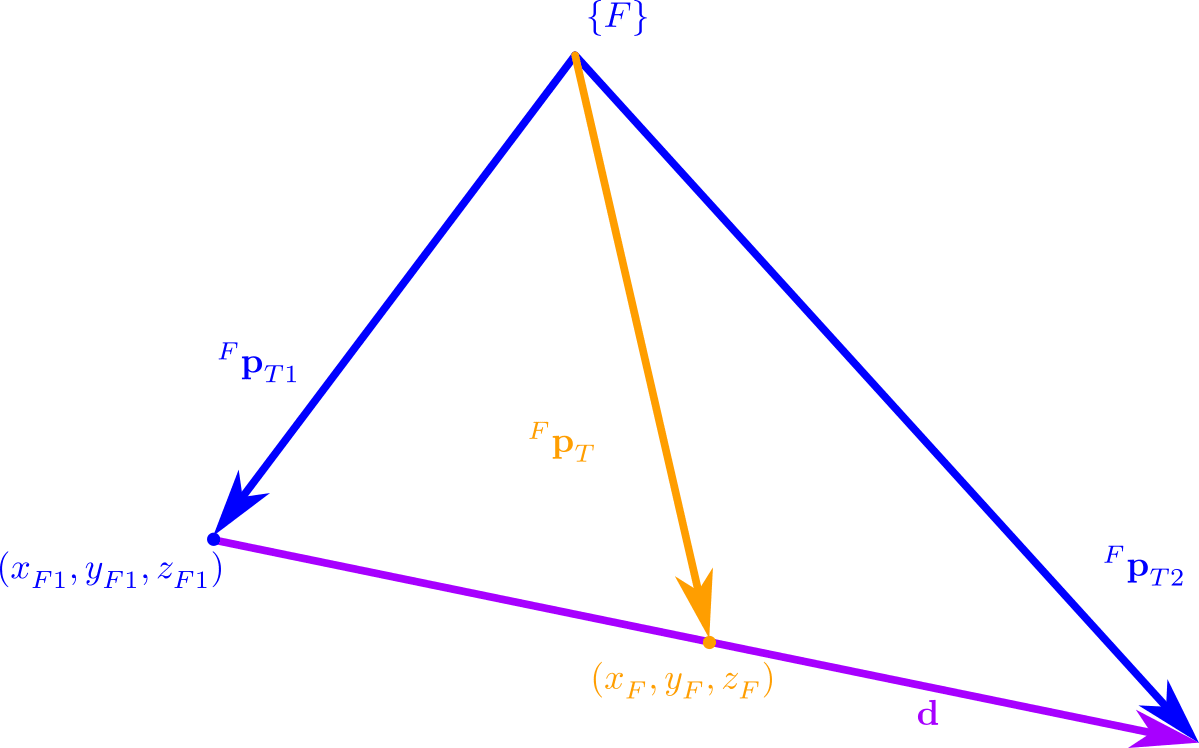
\includegraphics[width=10cm]{images/line-segment-trajectory-wrt-fulcrum.png}\\
\caption{Line segment trajectory of tool tip with respect to Fulcrum reference frame}
\end{figure}
\end{center}
\[
\mathbf{d} = {}^{F}\mathbf{p}^{}_{T2} - {}^{F}\mathbf{p}^{}_{T1} = [l, m, n]^\top
\]
\[
{}^{F}\mathbf{p}^{}_{T} = [x^{}_{F}, y^{}_{F}, z^{}_{F}]^\top
\]
\[
{}^{F}\mathbf{p}^{}_{T} = {}^{F}\mathbf{p}^{}_{T1} + s\mathbf{d}
\]
\[
s = \frac{x^{}_{F} - x^{}_{F1}}{l} = \frac{y^{}_{F} - y^{}_{F1}}{m} = \frac{z^{}_{F} - z^{}_{F1}}{n} \;\; s \in [0, 1]
\]

\begin{equation}
\begin{cases}
x^{}_{F} = sl + x^{}_{F1} = (1-s)x^{}_{F1} + sx^{}_{F2} \\
y^{}_{F} = sm + y^{}_{F1} = (1-s)y^{}_{F1} + sy^{}_{F2} \\
z^{}_{F} = sn + z^{}_{F1} = (1-s)z^{}_{F1} + sz^{}_{F2}
\end{cases}
\end{equation}

After having calculated the cartesian coordinates we can calculate the spherical coordinates using the \ref{eqns:cartesian-to-spherical} equations.

The line segment trajectory of tool tip, as analysed in this section needs no implementation as 
it is already implemented in the ROS MoveIt library and can be used by calling the method 
\textbf{computeCartesianPath}.

\subsubsection{Cubic Spline trajectory of tool tip}

A useful mathematical tool to construct a smooth curve that visits every point from a given set of waypoints are \textbf{cubic splines}. A cubic spline is 
constructed using smaller curves that are described by a polynomial of 3rd order. Let $\left\lbrace \mathbf{P}_0, \mathbf{P}_1, \ldots , \mathbf{P}_n \right\rbrace$ 
be a set of waypoints, where each point has coordinates $\mathbf{P}_i = [x_i, y_i, z_i]^\top$. Then between each 2 points a cubic 
polynomial can be constructed (one for each coordinate, 3 in total). The following equations are for the $x$-coordinate and in the exact same way one can 
calculate the cubic polynomials for the $y,z$ coordinates as well. For each pair of waypoints we want to calculate the following cubic polynomial
\begin{equation}
\label{cubic-polynomial}
x_i(s) = a_i(s-s_i)^3 + b_i(s-s_i)^2 + c_i(s-s_i) + d_i, \hspace{3em} s_i \leqslant s \leqslant s_{i+1}
\end{equation}

The polynomial in equation \ref{cubic-polynomial} has four unknowns which means that four additional equations are needed to get a unique solution and fully 
define the polynomial. These equations can be formed using the boundary conditions for the first and last point of each curve.
\begin{equation}
x_i(s_i) = x_i
\end{equation}
\begin{equation}
x_i(s_{i+1}) = x_{i+1}
\end{equation}
\begin{equation}
\dot{x}_i(s_i) = \dot{x}_i
\end{equation}
\begin{equation}
\dot{x}_i(s_{i+1}) = \dot{x}_{i+1}
\end{equation}

First we solve for $c_i$ and $d_i$, which can easily be calculated as follows
\begin{equation}
\label{di-eq}
d_i = x_i(s_i) = x_i
\end{equation}
and by taking the derivative of \ref{cubic-polynomial}, we can calculate $c_i$
\begin{equation}
\label{cubic-polynomial-first-derivative}
\dot{x}_i(s_i) = 3a_i(s-s_i)^2 + 2b_i(s-s_i) + c_i
\end{equation}
\begin{equation}
\label{ci-eq}
c_i = \dot{x}_i(s_i) = \dot{x}_i
\end{equation}

By substituting $s = s_{i+1}$ in \ref{cubic-polynomial} and \ref{cubic-polynomial-first-derivative}, by using equations \ref{ci-eq}, \ref{di-eq} and if 
we set $σ = s_{i+1}-s_i$ for brevity, we get the following two equations
\begin{equation}
\label{xi1}
x_{i+1} = x_i(s_{i+1}) = a_i σ^3 + b_i σ^2 + c_i σ + x_i
\end{equation}
and
\begin{equation}
\label{xdi1}
\dot{x}_{i+1} = \dot{x}_i(s_{i+1}) = 3a_i σ^2 + 2b_i σ + \dot{x}_i
\end{equation}

By multiplying \ref{xdi1} by $σ$ and \ref{xi1} by $-3$ and add them together we get
\[
\dot{x}_{i+1}σ - 3x_{i+1} = -b_iσ^2 -2\dot{x}_iσ - 3x_i
\]
\begin{equation}
b_i = \frac{1}{σ^2} (3x_{i+1} -3x_i - \dot{x}_{i+1}σ - 2\dot{x}_iσ)
\end{equation}

Similarly, by multiplying \ref{xdi1} by $σ$ and \ref{xi1} by $-2$ and add them together we get
\[
\dot{x}_{i+1}σ - 2x_{i+1} = a_iσ^3 -\dot{x}_iσ - 2x_i
\]
\begin{equation}
a_i = \frac{1}{σ^3} (\dot{x}_{i+1}σ - 2x_{i+1} + \dot{x}_iσ +2x_i)
\end{equation}

\begin{center}
\begin{figure}[H]
\centering
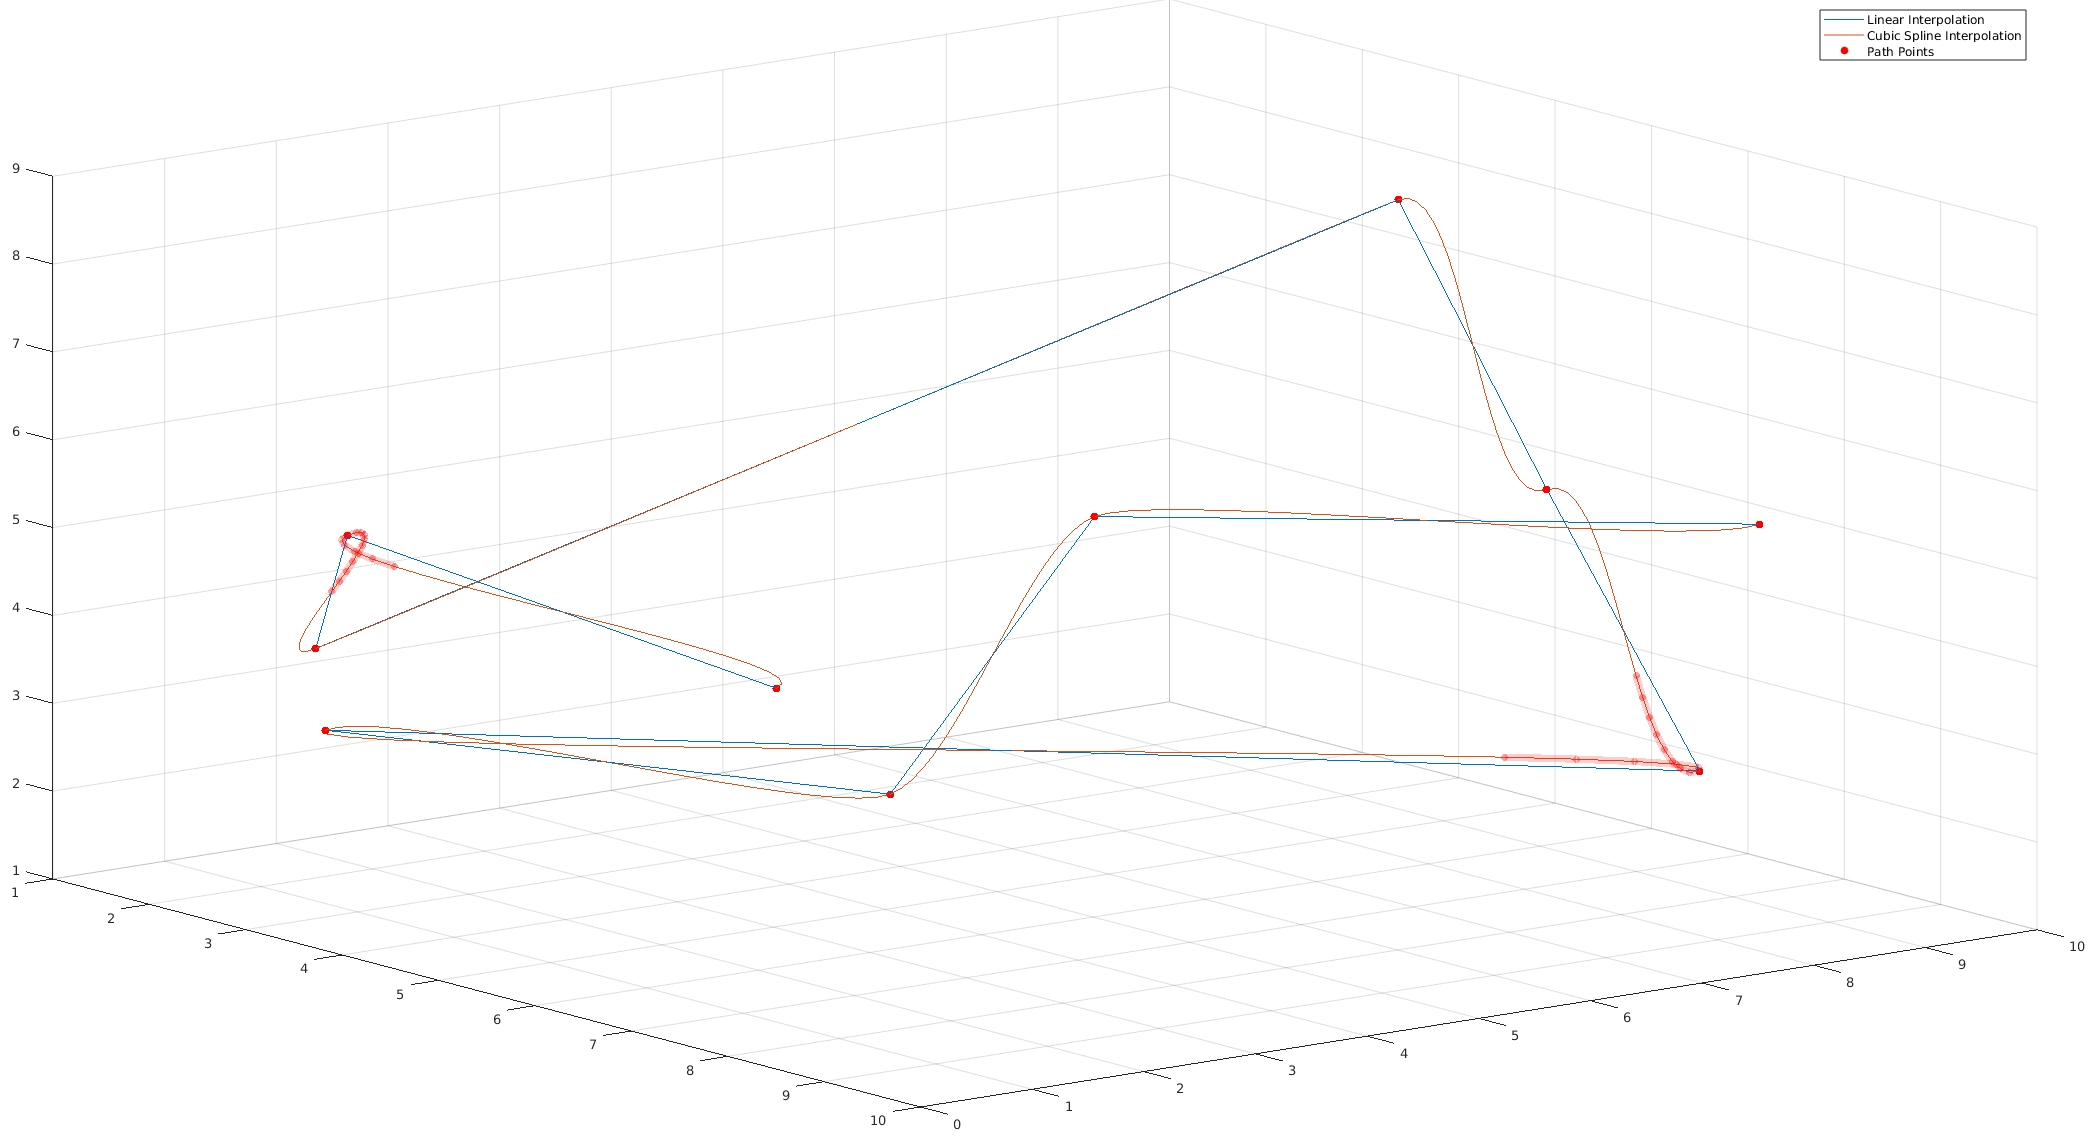
\includegraphics[width=\textwidth]{images/cubic-spline-path1.png}\\
\caption{Cubic Spline curve with 10 waypoints} 
\label{b-spline-explanation}
\end{figure}
\end{center}


\subsubsection{B-Spline trajectory of tool tip}

The \textbf{B-Splines} are smooth curves which are constructed from \textbf{B\'ezier} curves. A B\'ezier curve is a parametric smooth curve and is a $k$-th order interpolation of $k+1$ control points.

\begin{center}
\begin{figure}[H]
\centering
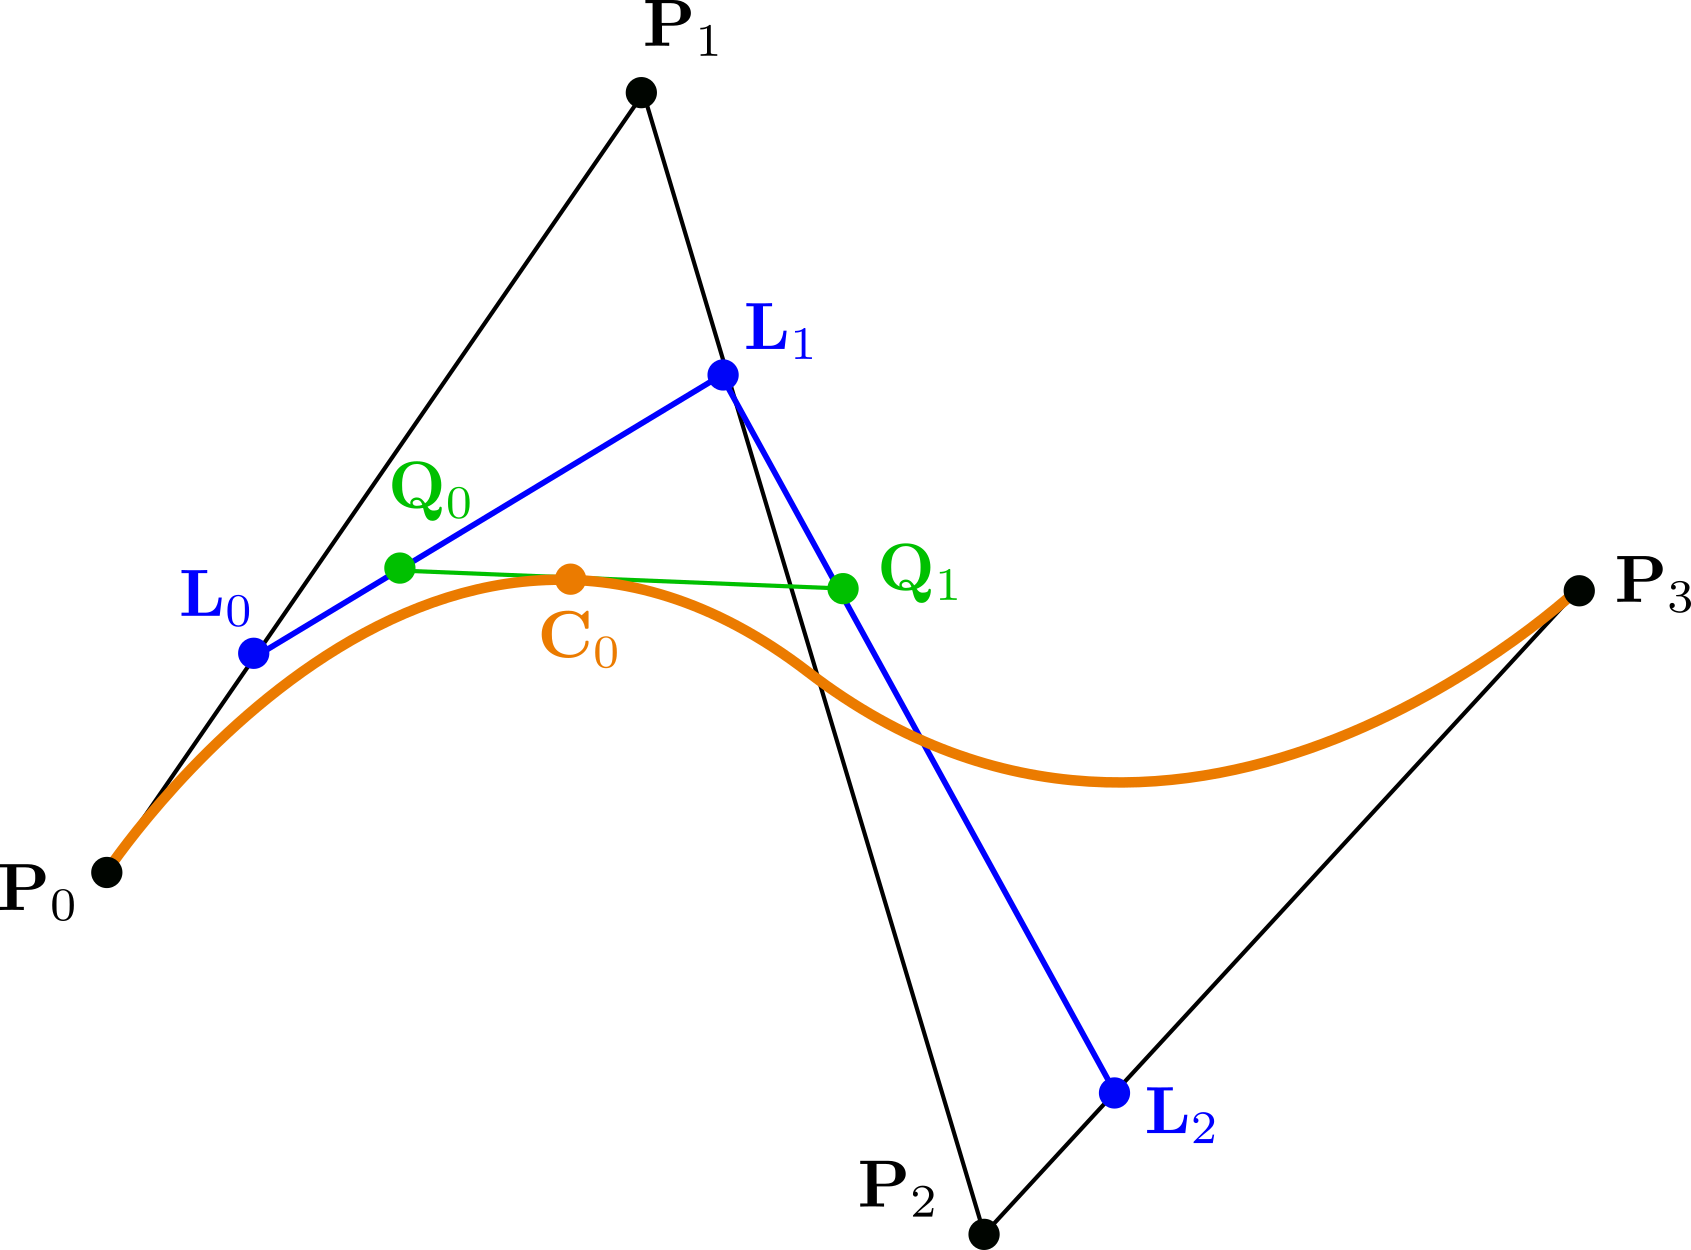
\includegraphics[width=0.5\textwidth]{images/bezier-curve.png}\\
\caption{Cubic B\'ezier curve calculated using cubic interpolation of 4 control points} 
\end{figure}
\end{center}

We first calculate the linear interpolation of the control points
\begin{equation}
\mathbf{L}_0(s) = (1-s)\mathbf{P}_0 + s\mathbf{P}_1
\end{equation}
\[
\mathbf{L}_1(s) = (1-s)\mathbf{P}_1 + s\mathbf{P}_2
\]
\[
\mathbf{L}_2(s) = (1-s)\mathbf{P}_2 + s\mathbf{P}_3
\]
The next step is to calculate the quadratic interpolation of the control points or equivalently, the linear interpolation of the previously calculated points $\mathbf{L}_0,\mathbf{L}_1,\mathbf{L}_2$
\[
\mathbf{Q}_0(s) = (1-s)\mathbf{L}_0(s) + s\mathbf{L}_1(s)
\]
\begin{equation}
\mathbf{Q}_0(s) = (1-s)^2\mathbf{P}_0 + 2(1-s)s\mathbf{P}_1 + s^2\mathbf{P}_2
\end{equation}
\[
\mathbf{Q}_1(s) = (1-s)^2\mathbf{P}_1 + 2(1-s)s\mathbf{P}_2 + s^2\mathbf{P}_3
\]
Similarly for the last step, we calculate the cubic interpolation of the control points or equivalently, the linear interpolation of the previously calculated points $\mathbf{Q}_0,\mathbf{Q}_1$
\[
\mathbf{C}_0(s) = (1-s)\mathbf{Q}_0(s) + s\mathbf{Q}_1(s)
\]
\begin{equation}
\mathbf{C}_0(s) = (1-s)^3\mathbf{P}_0 +3(1-s)^2 s\mathbf{P}_1 + 3(1-s)s^2\mathbf{P}_2 + s^3\mathbf{P}_3
\end{equation}

The cubic B\'ezier curve can also be calculated using the following more compact equation, in matrix form
\begin{equation}
\mathbf{C}_0(t) = \begin{bmatrix} \mathbf{P}_0 & \mathbf{P}_1 & \mathbf{P}_2 & \mathbf{P}_3 \end{bmatrix} 
\begin{bmatrix} 
-1 & 3 & -3 & 1 \\
3 & -6 & 3 & 0 \\
-3 & 3 & 0 & 0 \\
1 & 0 & 0 & 0
\end{bmatrix}
\begin{bmatrix}
s^3 \\ s^2 \\ s \\ 1
\end{bmatrix}
\end{equation}

A $k$-degree \textbf{B-Spline} curve defined by $n+1$ control points will consist of $n-k+1$ B\'ezier curves. For example if we want to construct a cubic B-Spline using 6 control points, then we will need to construct 
and connect together 3 B\'ezier curves.

\begin{center}
\begin{figure}[H]
\centering
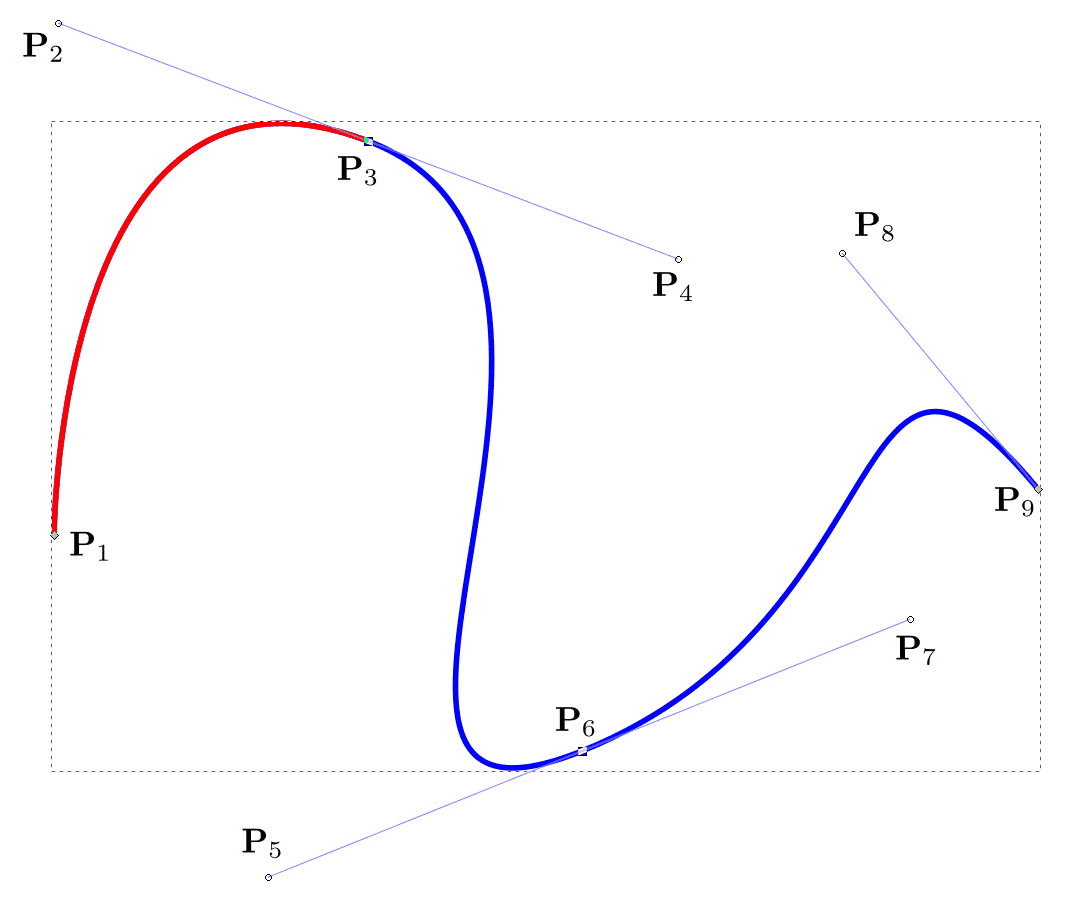
\includegraphics[width=0.6\textwidth]{images/b-spline-explanation.png}\\
\caption{B-Spline curve constructed from 3 B\'ezier curves. The first B\'ezier curve colored in red is a quadratic one and the following two are both cubic.} 
\label{b-spline-explanation}
\end{figure}
\end{center}

In most cases the B-Spline curves are constructed by starting from a quadratic B\'ezier curve, which is constructed from 3 control points and then all other 
parts of the curve are constructed from cubic B\'ezier curves, each constructed from 4 control points. As shown in figure \ref{b-spline-explanation}, the B-Spline 
curves do not pass from all control points. This means that if we have a path formed by a set of waypoints and we want the robot to pass from all of them, then 
in order to construct a B-Spline trajectory we will need additional intermediary points. The first and last points are part of the curve and the other control 
points are not. If no additional points can be calculated then the robot will not pass from all the points, which in some cases is also acceptable and useful.

\begin{center}
\begin{figure}[H]
\centering
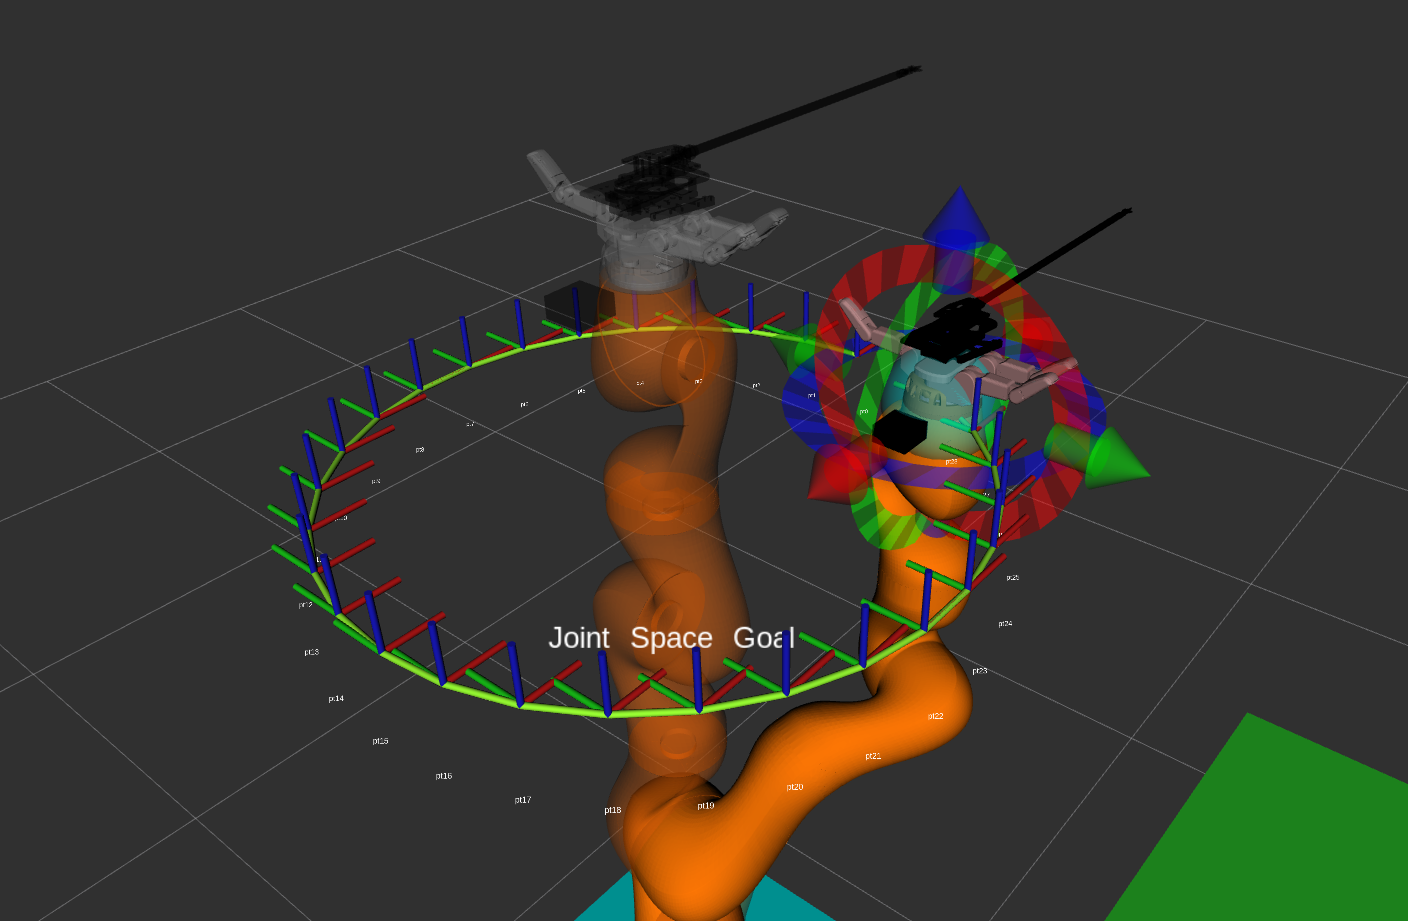
\includegraphics[width=0.7\textwidth]{images/simple_circular_traj1.png}\\
\caption{Circlular trajectory around the z axis of the home position of the robot}
\label{fig:circ-traj-out-of-angle-range}
\end{figure}
\end{center}

It is very important that the designed trajectory respects the joints angles' range. For example
depending on the starting position of the circular trajectory depicted at figure 
\ref{fig:circ-traj-out-of-angle-range}, the robot arm may reach it's joint bounds and in order to 
continue executing the trajectory it will have to make a sudden jump to reset the angles. 
This could have serious side-effects for both the surgical task and thus the patient, as well as 
for the operating staff, who control the robot.


\subsection{Trajectory planning in joint angles space}

\begin{center}
\begin{figure}[H]
\centering
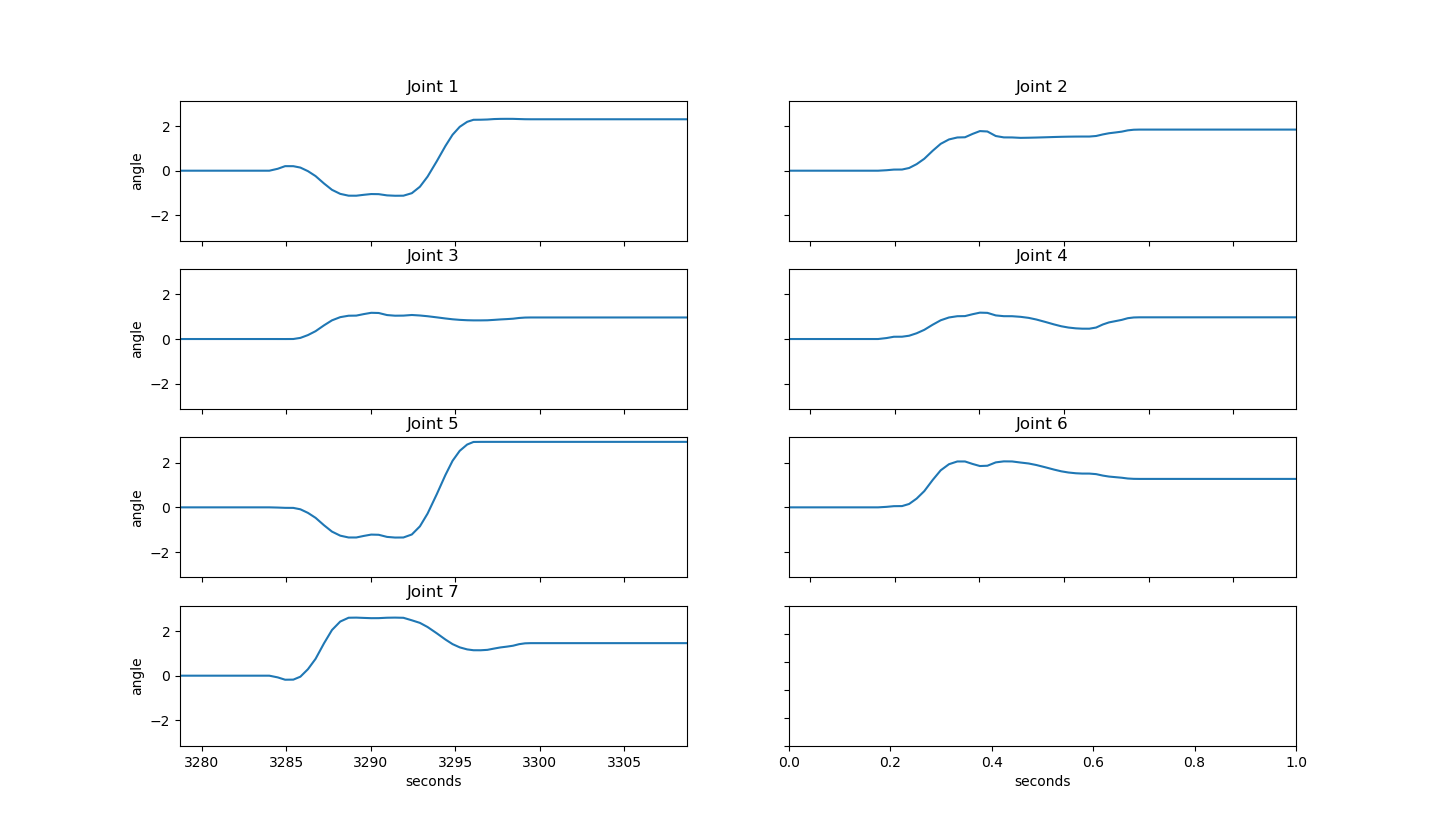
\includegraphics[width=\textwidth]{images/trajectory1-test1.png}\\
\caption{Trajectory diagrams in joints space.}
\end{figure}
\end{center}


\subsubsection{Polynomials of 5th order}


\subsubsection{Trapezoidal velocity profile}


\subsubsection{S-Curve velocity profile}
\chapter{System Control}

\section{RCM Tracking}
\label{section:rcm-tracking}

This section describes how to use a Remote Center of Motion error metric in order to implement a control system that makes sure that the laparoscopic tool is always aligned with the fulcrum point and it satisfies the RCM 
constraint. To calculate this error, which can then be used as a feedback signal to a control system, the line of the long axis of the surgical tool must be first defined. To define this line, 2 points are needed. Both of these 
points can be calculated using the transformation of the surgical tool, which is attached to the robot's TCP on the end-effector. Let the following be the pose of the surgical tool with respect to the global reference frame
\begin{equation}
{}^UT_{T0} = \begin{bmatrix}
\mathbf{\hat{x}} & \mathbf{\hat{y}} & \mathbf{\hat{z}} & \mathbf{p} \\
0                & 0                & 0                & 1 \\
\end{bmatrix}
\end{equation}
Using this pose, let $A,B$ be the points such that 
\begin{equation}
\overrightarrow{O_FA} = \mathbf{p}, \quad \textrm{and} \quad \overrightarrow{O_FB} = \mathbf{p} + \mathbf{\hat{x}}
\end{equation}
where $O_F$ is the origin point of the fulcrum reference frame. The the line of interest is defined as the line $l$ that passes through the points $A$ and $B$. \\

The alignment error is calculated using a known position and orientation for the second fulcrum reference frame. In real-case scenarios the exact position and orientation of the fulcrum points are not precisely known 
but can be estimated. To model the uncertainty of the pose, the pose message of the fulcrum point includes also a covariance matrix. The ROS message that was used was the \textbf{PoseWithCovarianceStamped} which needs the 
following information (with respect to the global frame) to be fully defined:
\[
( \mathbf{p}, \mathbf{q}, \mathbf{C} ), \quad \mathbf{p} \in \mathbb{R}^3, \mathbf{q} \in \mathbb{H}, \mathbf{C} \in \mathbb{R}^{6 \times 6}
\]
where 
\begin{equation}
\mathbf{C} = \begin{bmatrix}
σ_{xx} & σ_{xy} & σ_{xz} & σ_{xψ} & σ_{xθ} & σ_{xφ} \\
σ_{xy} & σ_{yy} & σ_{yz} & σ_{yψ} & σ_{yθ} & σ_{yφ} \\
σ_{xz} & σ_{yy} & σ_{zz} & σ_{zψ} & σ_{zθ} & σ_{zφ} \\
σ_{xψ} & σ_{yψ} & σ_{zψ} & σ_{ψψ} & σ_{ψθ} & σ_{ψφ} \\
σ_{xθ} & σ_{yθ} & σ_{zθ} & σ_{ψθ} & σ_{θθ} & σ_{θφ} \\
σ_{xφ} & σ_{yφ} & σ_{zφ} & σ_{ψφ} & σ_{θφ} & σ_{φφ} \\
\end{bmatrix}
\end{equation}
The covariance matrix and its coefficients can be calculated using equations \ref{eq:cov-matrix} and \ref{eq:cov-matrix-coeff}, using the mean values of the estimations of $x,y,z,ψ,θ,φ$.

\begin{center}
\begin{figure}[!htb]
\centering
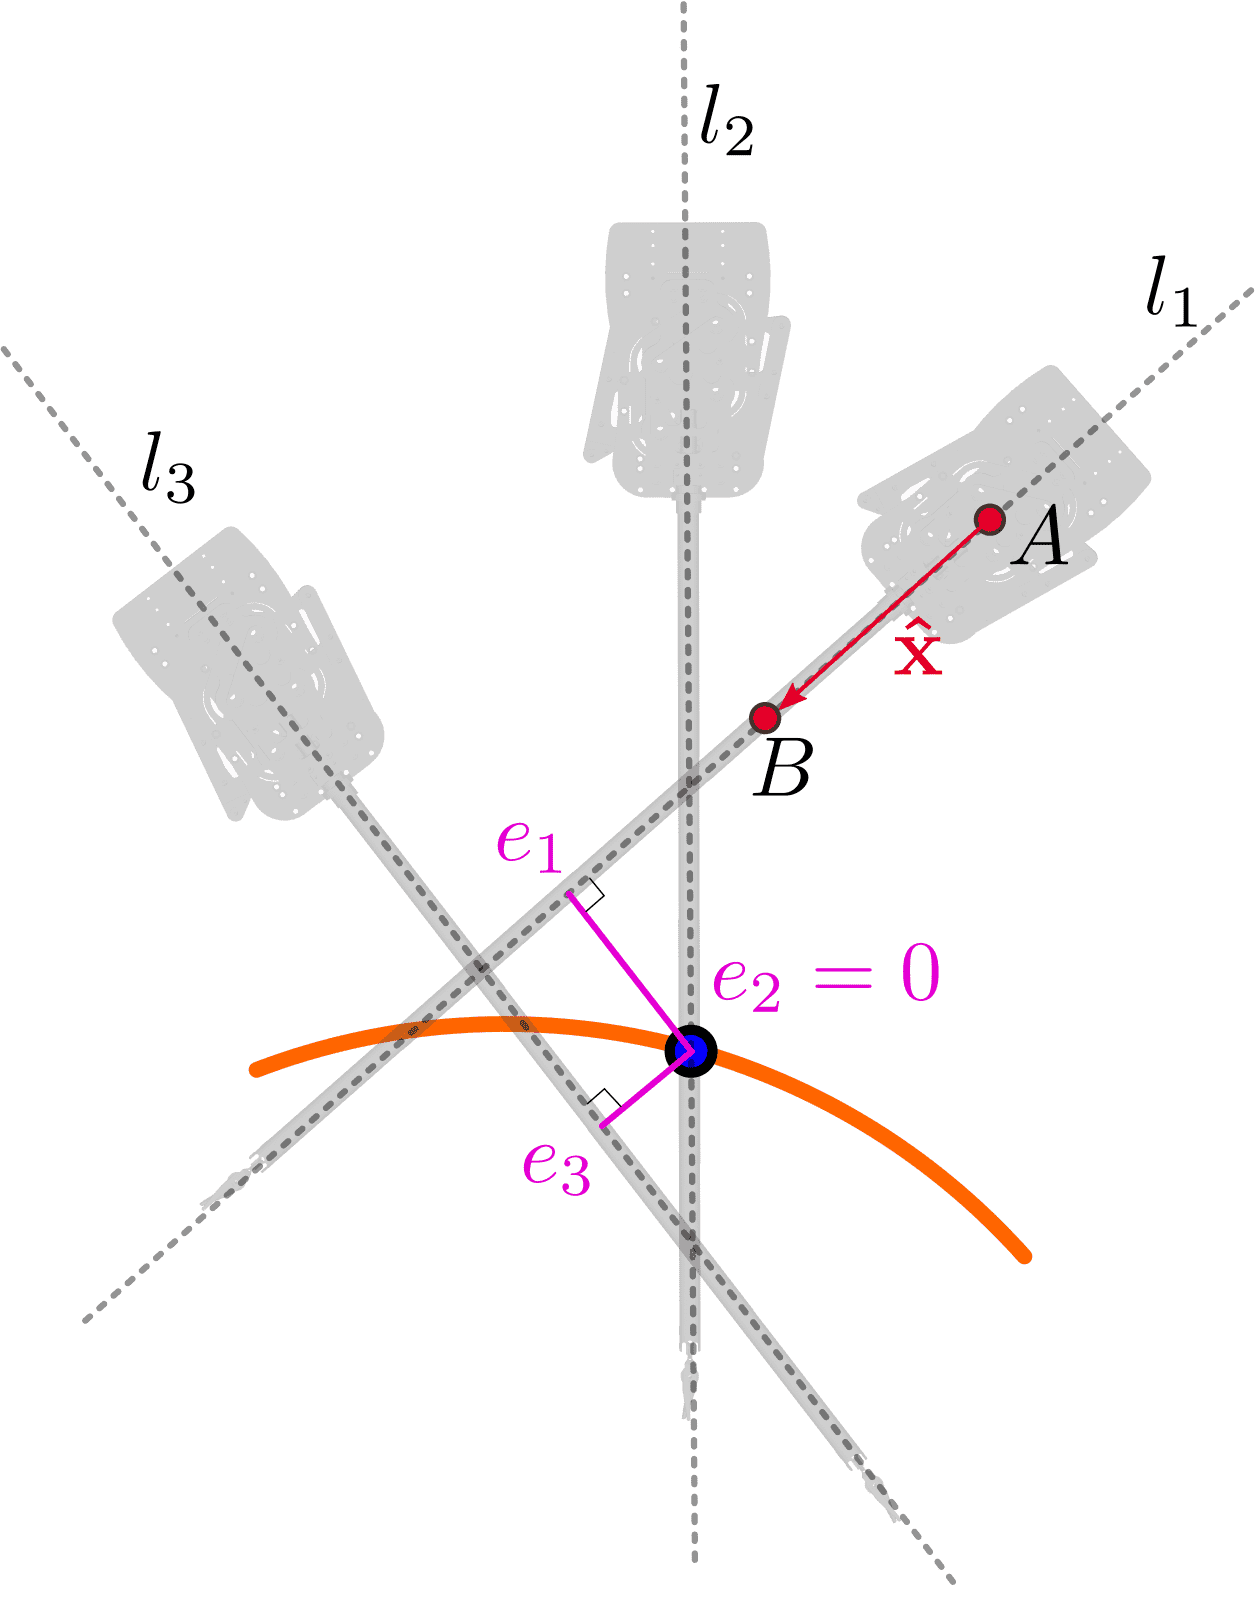
\includegraphics[width=0.5\textwidth]{images/robot_planner6/rcm-error-geometry.png}
\caption{Geometric calculation of the RCM alignment error $e$ using the distance between the line $l$ and the RCM (aka Fulcrum) point.}
\label{rcm-error-geometry}
\end{figure}
\end{center}

Since both the origin of the fulcrum reference frame and the line of the long axis of the tool are known then the alignment error can be calculated as the distance of the line $l$ from the point $O_F$
\begin{equation}
e_{rcm} = d(l, O_F)
\end{equation}

To calculate the distance $d(l, O_F)$ there is available a method in the \textbf{Eigen} C++ library that calculates the distance of a line that passes through 2 points, from a third point. Alternatively, this distance 
can be calculated using \ref{line-point-distance-formula}.
\begin{equation}
\label{line-point-distance-formula}
d(l, O_F) = \frac{\Vert \overrightarrow{O_FA} \times \mathbf{\hat{x}} \Vert}{\Vert \mathbf{\hat{x}} \Vert}
\end{equation}

Similar approaches to calculate this error/distance are presented in bibliography at \cite{Dong2016RobustTD} and \cite{Bauzano2009ControlMF}.\\

\begin{center}
\begin{figure}[!htb]
\centering
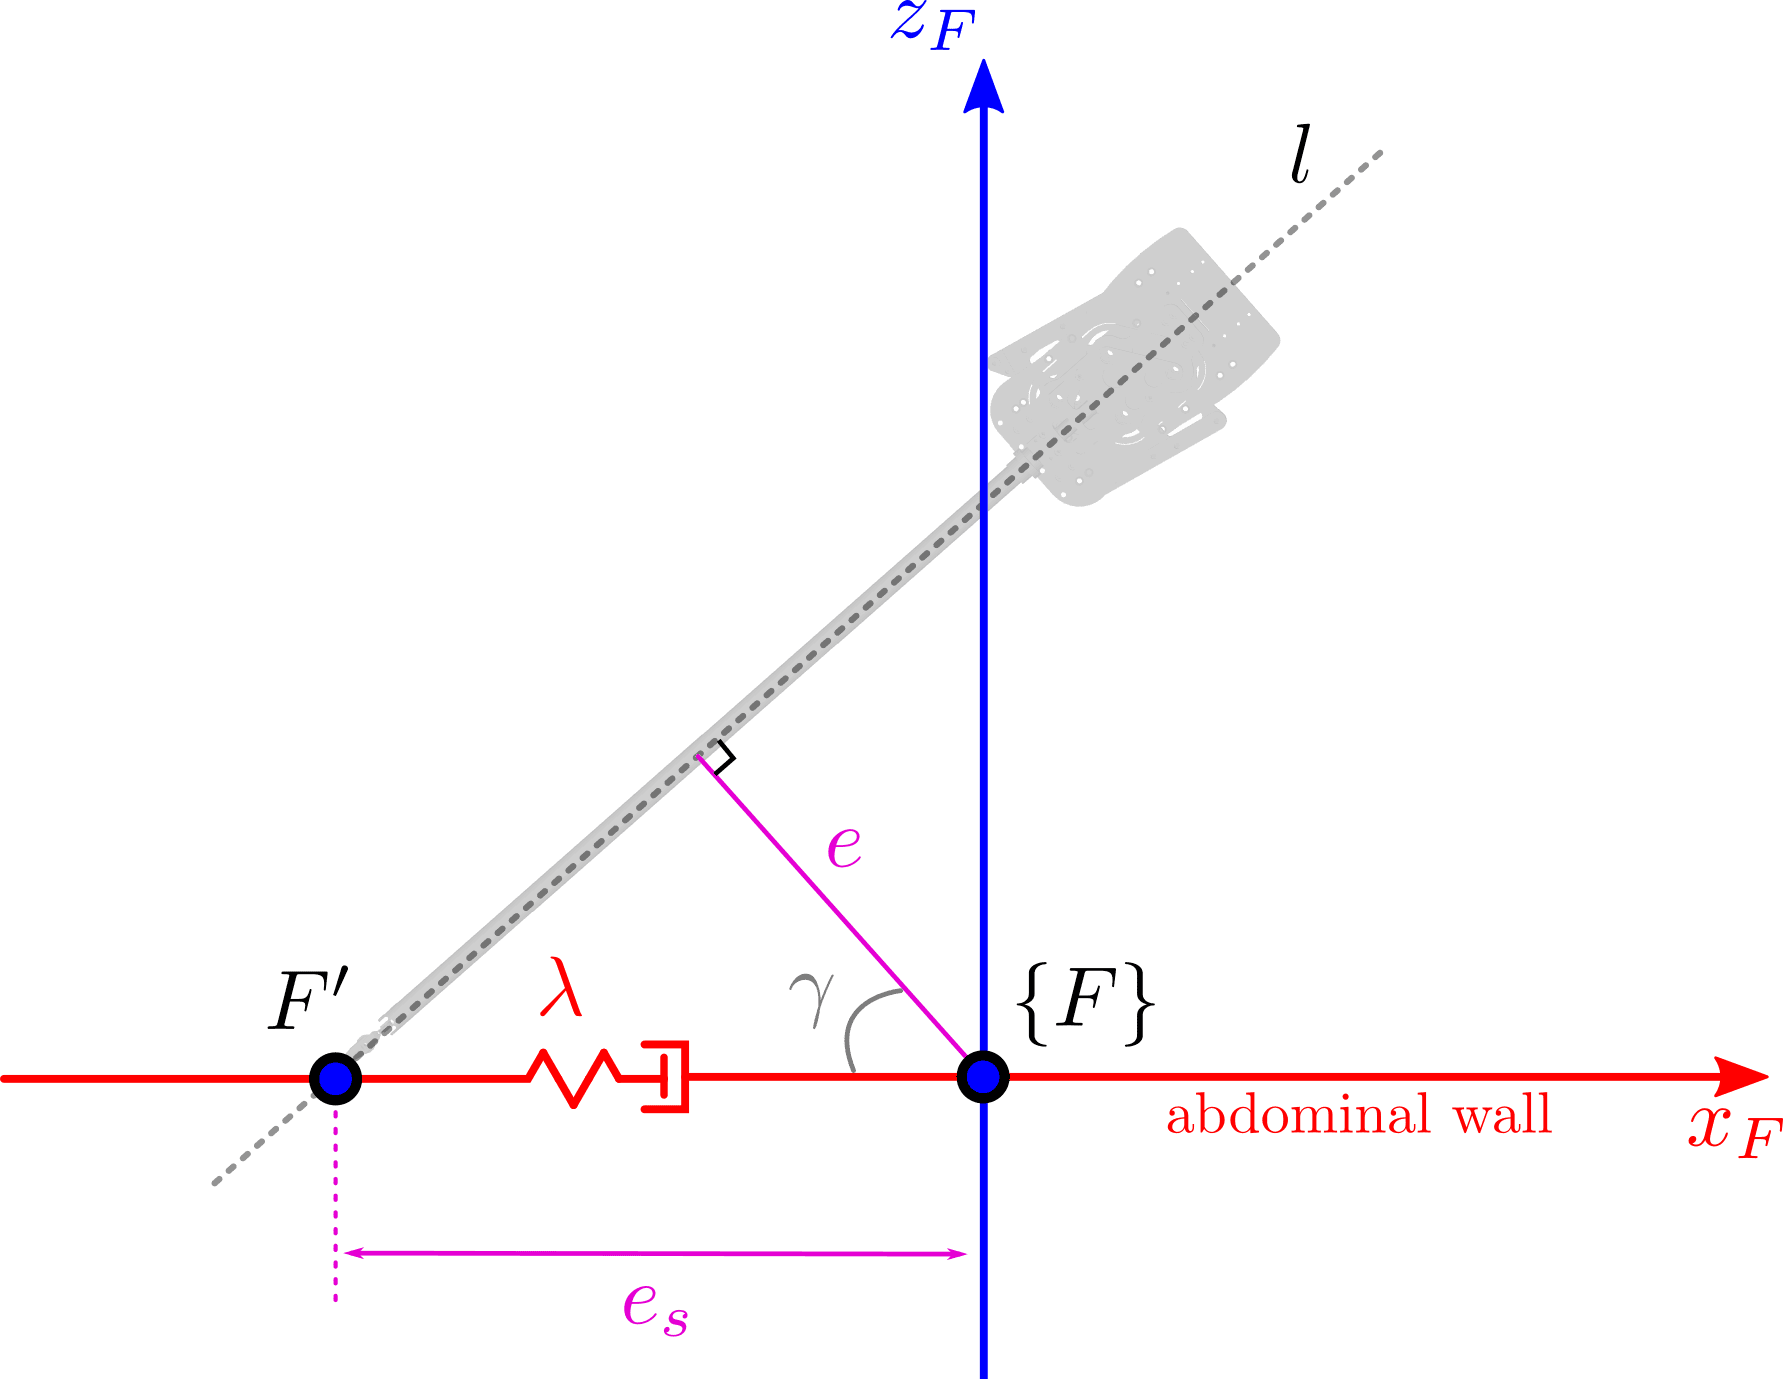
\includegraphics[width=0.5\textwidth]{images/rcm-force-interaction-model.png}
\caption{Force interaction model of the laparoscopic tool and the abdominal wall around the fulcrum point (RCM point)}
\label{rcm-force-interaction-model}
\end{figure}
\end{center}


If $e_{rcm} \leq 3_{max} = 1mm$ then the surgical tool axis passes through the fulcrum point and executes RCM trajectories, otherwise the robot is considered to have slipped from alignment, it does not execute RCM motion and 
probably generates a force $f \propto e$ which exerts pressure to the incision point and the abdominal wall (or the tissue around the incision point), which can have negative side-effects in the recovery of the incision.
In paper \cite{Bauzano2009ControlMF} a different distance $e_s$ is calculated as the RCM error as shown in figure \ref{rcm-force-interaction-model}, which is along the x-axis of the fulcrum reference frame or the axis 
of the abdominal wall (we assume local to the Fulcrum point the abdominal wall is a straight line). Using this deviation distance $e_s$ the force interaction between the surgical tool and the abdominal wall can be modelled 
with the following force

\begin{equation}
\Vert \mathbf{f}_s \Vert = λ e_s
\end{equation}
where $λ$ is the elasticity of the abdominal wall and can be measured experimentally and
\begin{equation}
e_s = \frac{1}{cosγ} e
\end{equation}

\begin{center}
\begin{figure}[!htb]
\centering
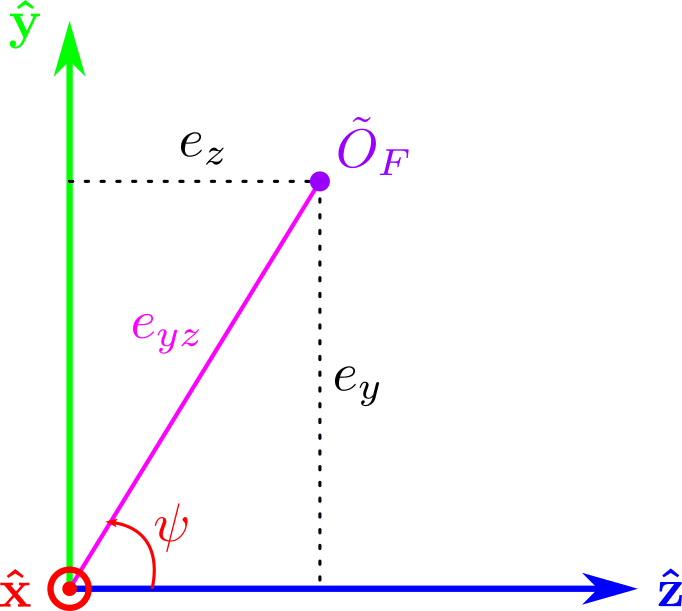
\includegraphics[width=0.4\textwidth]{images/rcm-error-yz.png}
\caption{RCM error calculation in yz plane. The RCM error or yz-error is the distance between the line of the $\mathbf{\hat{x}}$ vector (here seen as a point) and the estimated position of the origin of the
fulcrum reference frame $\tilde{O}_F$}
\label{rcm-error-yz-plane}
\end{figure}
\end{center}

The error $e_{rcm}$ can provide further information if the distance of the line $l$ (or of the $\mathbf{\hat{x}}$ axis) from the fulcrum point, is seen from a different perspective than that of 
figure \ref{rcm-error-geometry}. If this distance is seen from a plane that is perpendicular to $\mathbf{\hat{x}}$, then the line is seen as a point and the distance $d(l, O_F)$ is seen as a distance between 2 points, 
as illustrated in figure \ref{rcm-error-yz-plane}. This perspective of the RCM error (will also be referenced as yz-error $e_{yz}$) is more useful because it decomposes the error distance in 2 components that can be used to 
correct the goal pose of the robot so that is fixes the RCM misalignment.

\begin{equation}
e_y = e_{yz}sinψ \quad \textrm{and} \quad e_z = e_{yz}cosψ
\end{equation}

The angle $ψ$ that is used to split $e_{rcm}$ in the two components, is already known from the robot's pose and it is the yaw (also known as spin) angle of the surgical tool.\\

Using the estimated RCM error $\tilde{e}_{rcm}$ and the estimated position of the origin of the fulcrum reference frame, then an adaptive motion control system can be designed that corrects the trajectory to avoid RCM 
misalignment. The proposed control system is illustrated in the block diagram \ref{rcm-control-system-block-diagram} and a similar pivoting motion control system is also described in the bibliography 
in \cite{Muoz2005PivotingMC}.

\begin{center}
\begin{figure}[!htb]
\centering
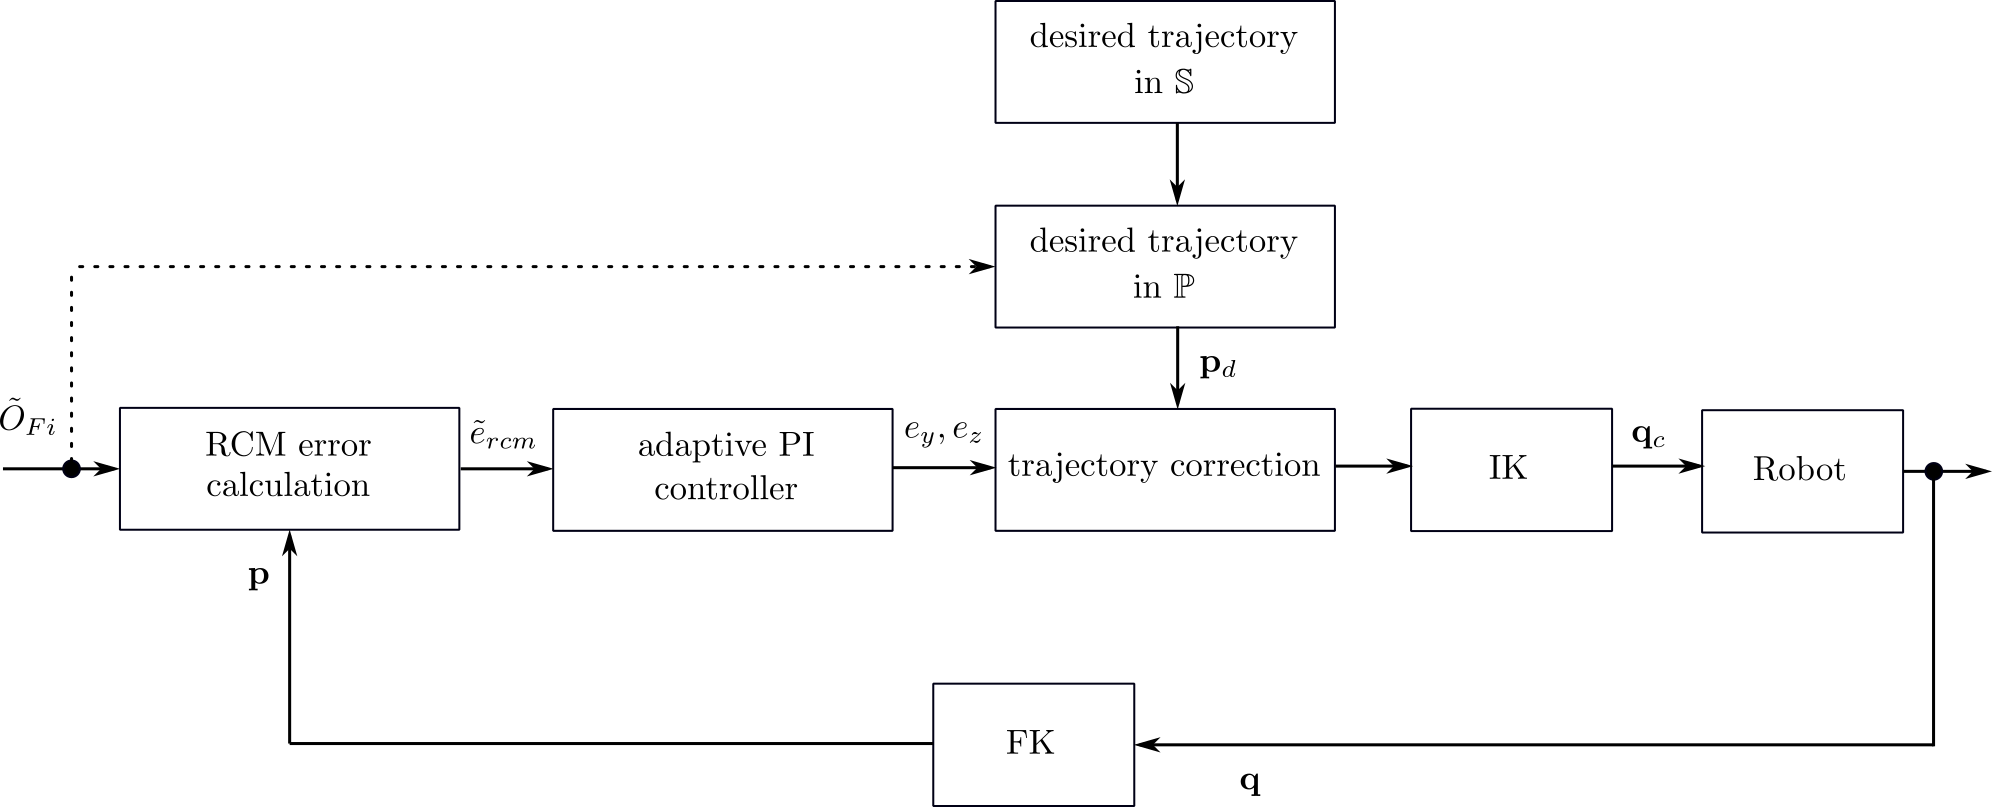
\includegraphics[width=\textwidth]{images/rcm-system-control.png}
\caption{RCM tracking proposed control system. The RCM error is used as input in the trajectory generator to correct the trajectory command in order to fix the RCM misalignment}
\label{rcm-control-system-block-diagram}
\end{figure}
\end{center}


\section{Visual Servoing}

At this chapter we briefly investigate how visual servoing can be applied in surgery robotics. \textbf{Visual Servoing} is the use of visual information 
to guide and control a robot. The main task of visual servoing is to control the end-effector's pose using features extracted from visual information. The 
features that are usually extracted from cameras are the position and orientation of the detected object, the distance of the object from the camera (using 
stereoscopic vision, photogrammetry or other techniques), the size and the shape of the object. The visual servoing can be executed either in the robot's space 
using position-based servoing or in the camera's space (also known as "pixel space") by using the image-based technique.

\subsection{Position based servoing}

\begin{center}
\begin{figure}[!htb]
\centering
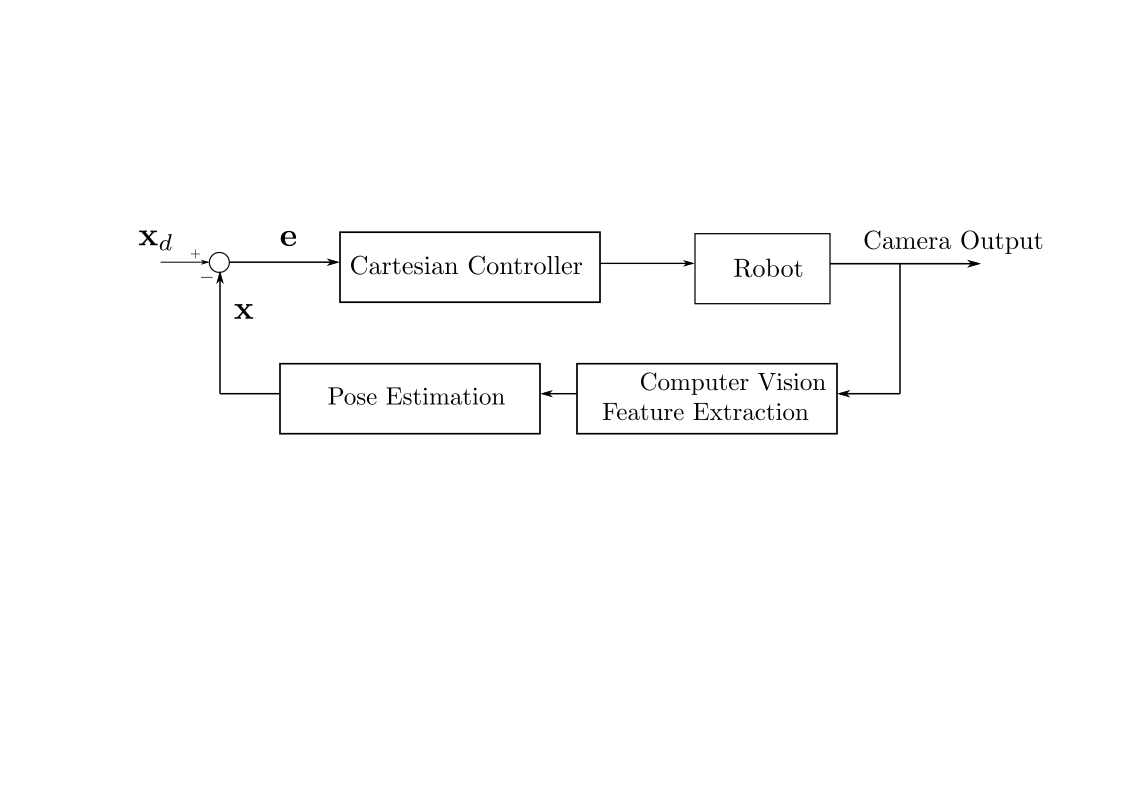
\includegraphics[width=0.8\textwidth]{images/visual-servoing-position-based.png}\\
\caption{Position based visual servoing closed loop control}
\end{figure}
\end{center}

\begin{itemize}
\item \textbf{Photogrammetric technique}
\item \textbf{Stereoscopic vision}: This methodology uses two separate views of the scene as taken from two viewports (from two cameras) 
and calculates the depth of various objects and areas using information from both views. For more details about stereoscopic vision see chapter \ref{stereoscopic-vision}
\item \textbf{Extracting depth from motion} This methodology is very similar to stereoscopic vision and is also known as \textit{monocular} or \textit{motion stereo}. The difference is that instead of using two views fromtwo distinct cameras this methodology 
uses two views from the same camera but from different points in time. A very important assumption for this methodology is to assume that two consecutive views from the video frame do not change significantly, so that some feature points can be matched in both views in order to calculate the depth information. This methodology 
is cheaper in terms of hardware but it fails to extract depth informations in cases where the robot is completely still.
\item \textbf{Servoing using 3D sensors}
\end{itemize}

\begin{center}
\begin{figure}[!htb]
\centering
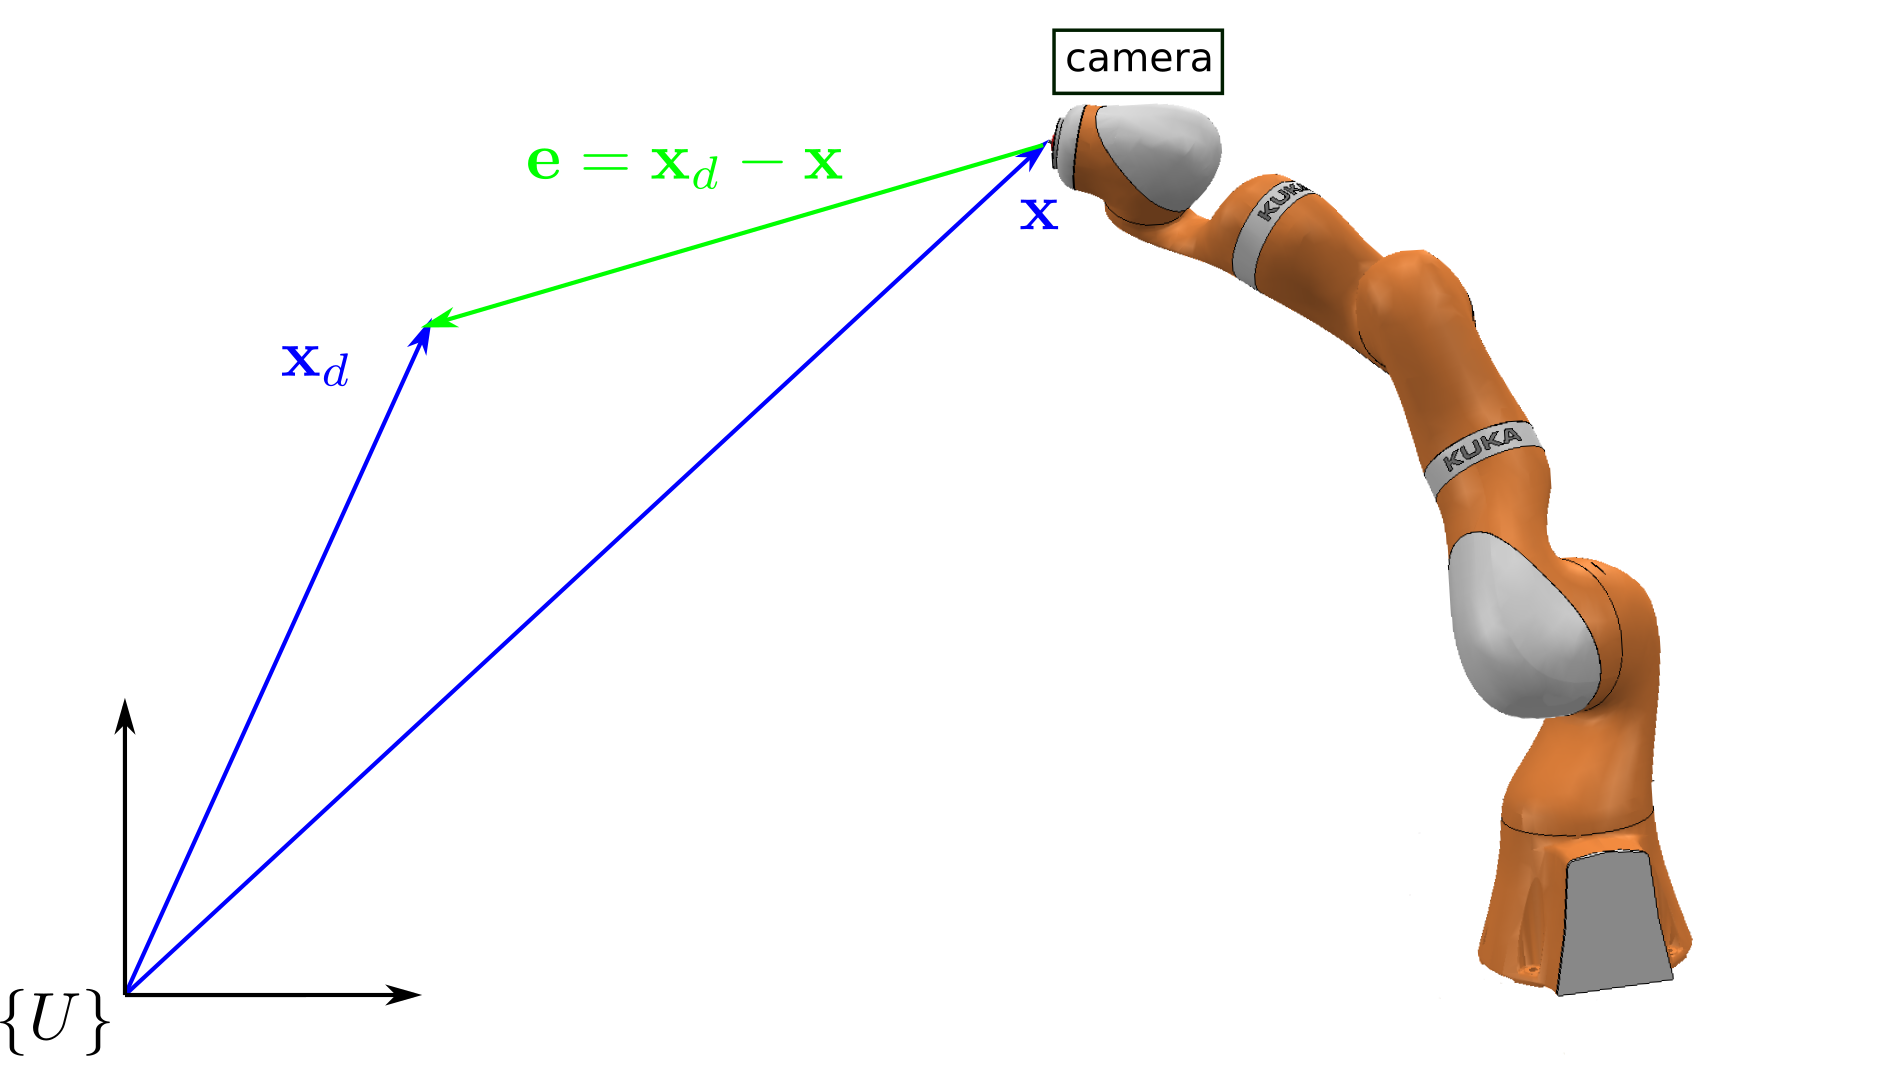
\includegraphics[width=0.6\textwidth]{images/visual-servoing-position-based2.png}\\
\caption{Position based visual servoing using depth from motion, stereo vision or 3D sensors, from which the desired position $\mathbf{x}_d$ is calculated and 
used to drive the robot.}
\end{figure}
\end{center}

\subsection{Image based servoing}

Image based servoing is a methodology for controlling a robot by directly using features extracted from the image as well as positions on the image plane. The goal of this methodology is 
to drive the robot in such a way so that the video frame is changed from an initial view to a final, desired view (see figure \ref{image-based-servoing-start-end} left and right frames). The commands 
that are sent to the robot from this methodology are defined in image space and not in the robot's task space. Moreover the distances calculated in image space are not directly related to distances 
in task space.

\begin{center}
\begin{figure}[!htb]
\centering
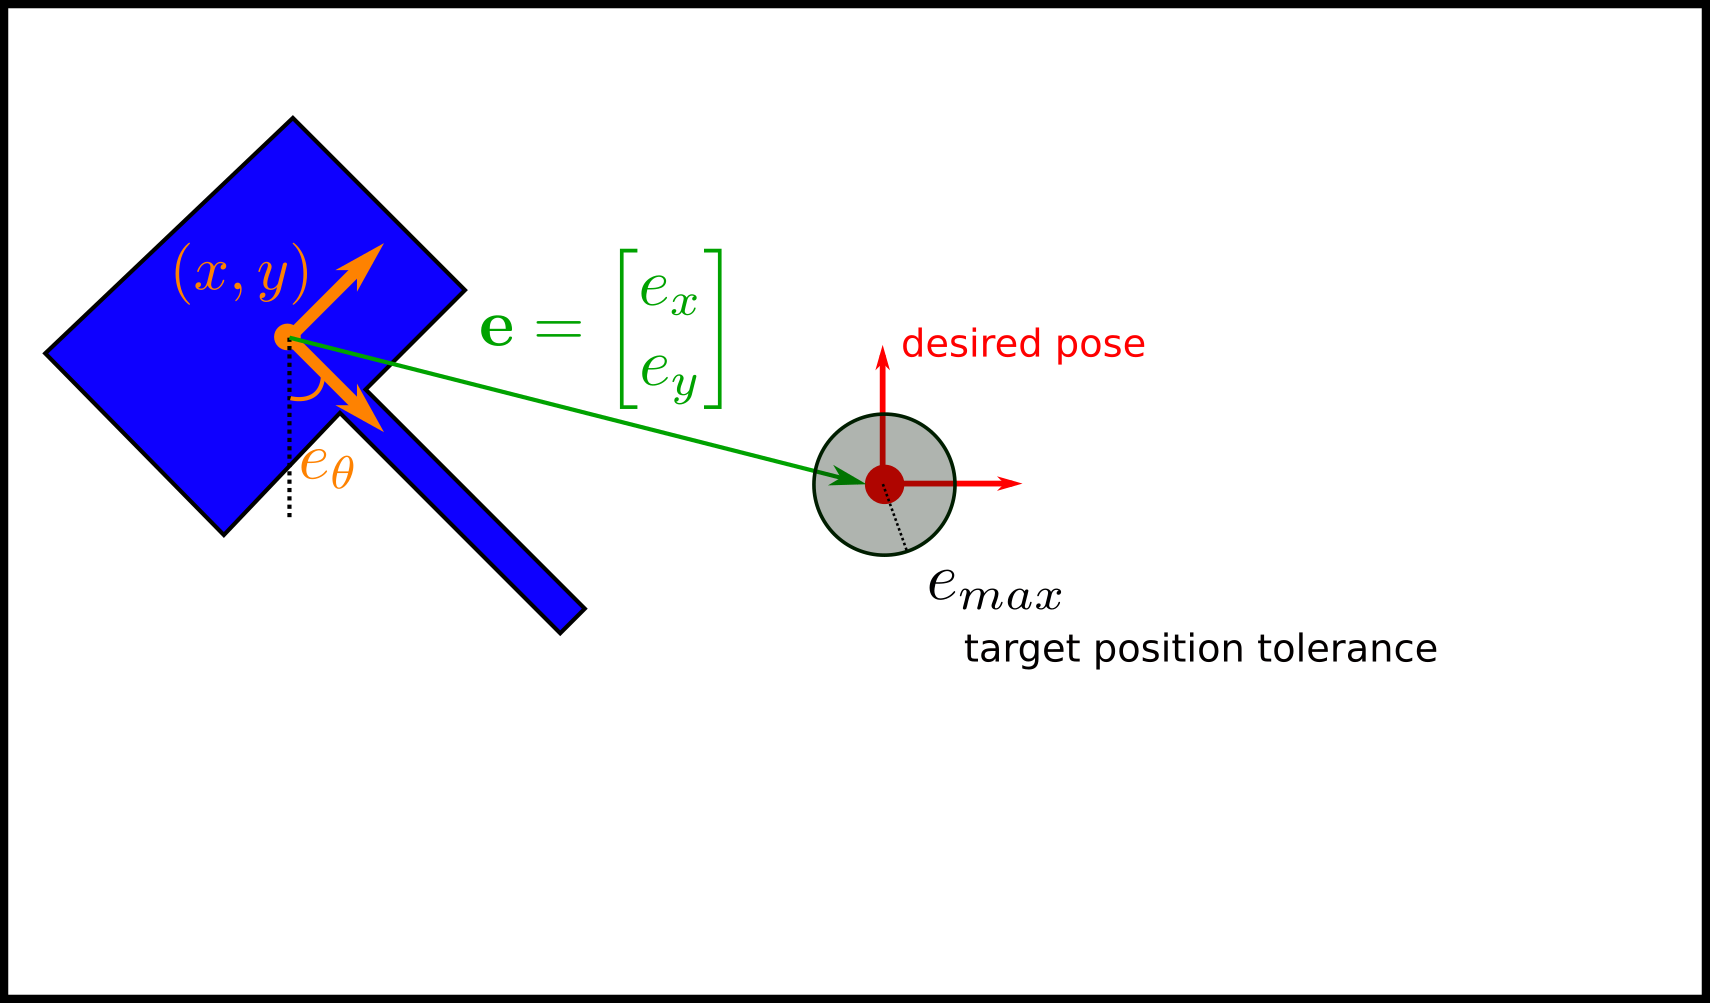
\includegraphics[width=0.45\textwidth]{images/visual_servo_start.png}
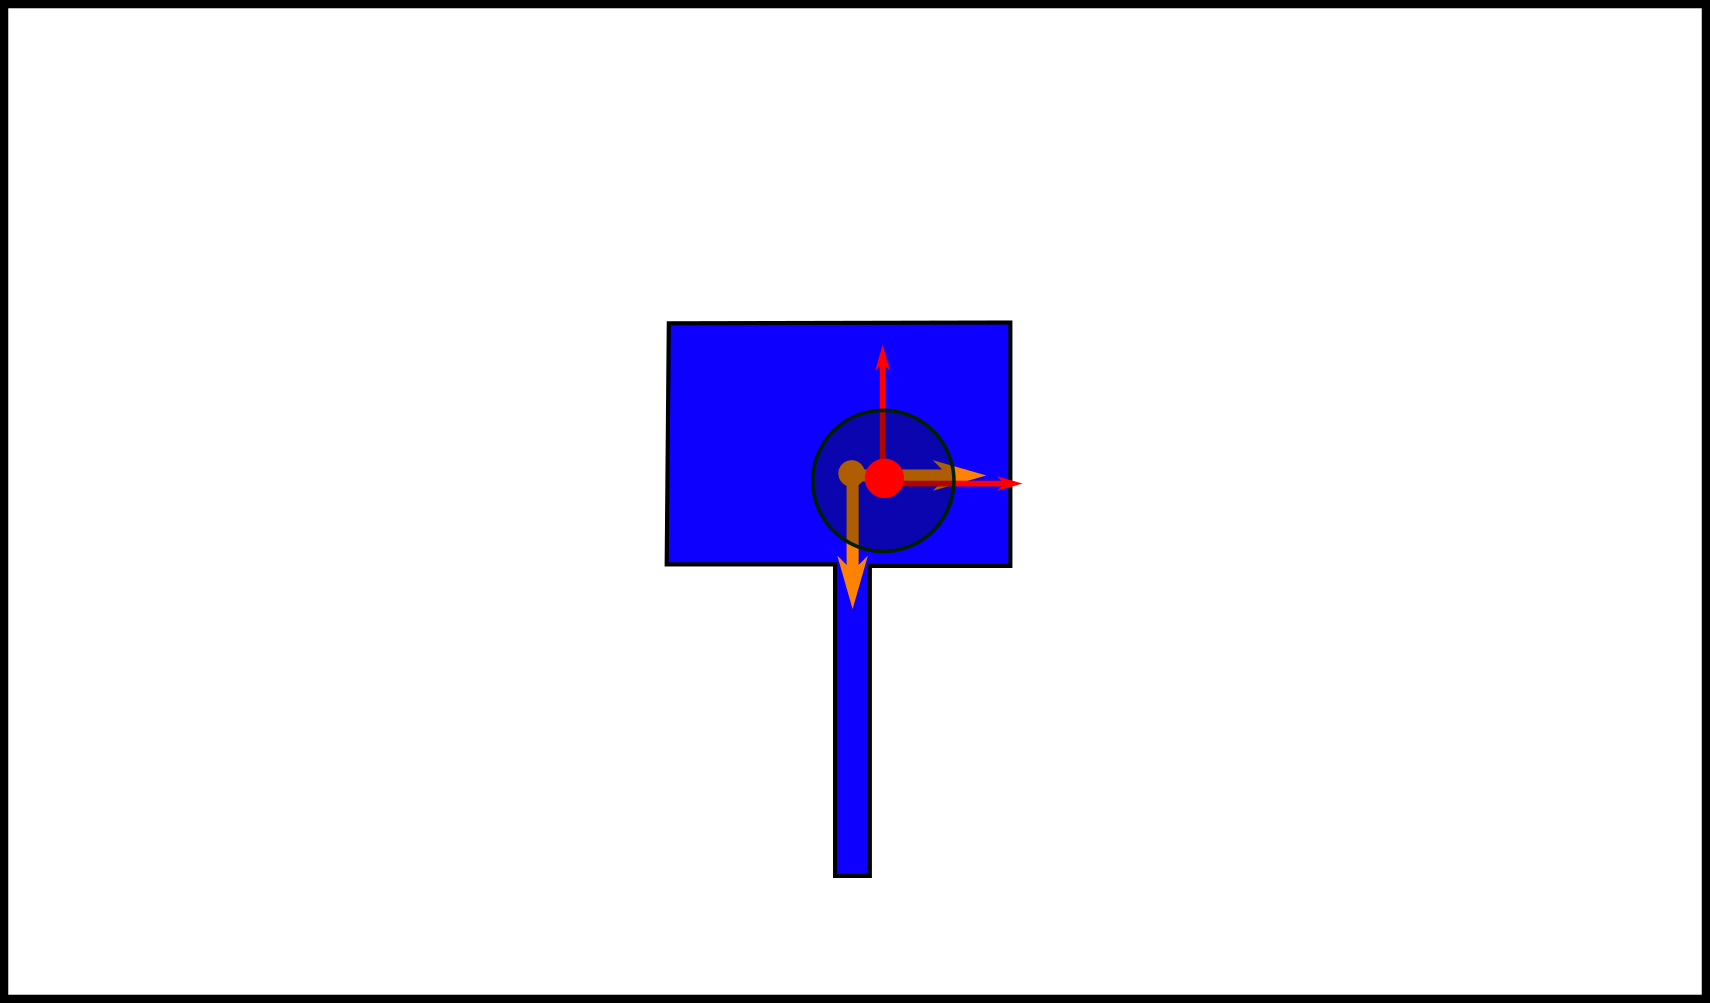
\includegraphics[width=0.45\textwidth]{images/visual_servo_end.png}\\
\caption{Image based visual servoing. The robot arm is controlled using the information gained from the video frames. The frames are 2Dimensional and thus 
the detected objects can have only 3 degrees of freedom which means we can mainly control 3 independent variables, here the $x,y,θ$ variables. The left image 
is the initial frame and the right image is the frame where the object is at the target pose.}
\label{image-based-servoing-start-end}
\end{figure}
\end{center}

The image based visual servoing control system as depicted in figure \ref{visual-servoing-image-based-control} consists of the \textbf{Image Controller}, the \textbf{Plant} (robot) and the \textbf{feedback term}. The Image controller is a simple 
\textbf{PD Controller} (PID can also be used, but in servo systems PD is more common) which outputs commands to be executed in the plant. These commands are not to be confused with the robot's internal controller commands. 
These commands are to be used to control the robot in task space, whereas the internal controller drives each joint to the desired angle. The feedback used to calculate the error for the controller, uses the camera's 
output and based on that it calculates the vector from the detected tool's center of mass to the center of the image frame (feature extraction).

\begin{equation}
\mathbf{x}[(k+1)T] = \mathbf{x}[kT] + \mathbf{u}[kT]
\end{equation}

where $\mathbf{x}[kT] = [x, y, z, θ, φ, ψ]^\top$ and the discrete PID control law is given by equation \ref{discrete-pid-control-law}
\begin{equation}
\label{discrete-pid-control-law}
\mathbf{u}[kT] = K_p \left[ \mathbf{e}[kT] + \frac{T}{T_i} \sum_{i=0}^{k-1} \mathbf{e}[iT] + \frac{T_d}{T} \left( \mathbf{e}[kT] - \mathbf{e}[(k-1)T] \right) \right]
\end{equation}

where $\mathbf{e}[kT] = [e_x, e_y, e_z, e_θ, e_φ, e_ψ]^\top$.

\begin{center}
\begin{figure}[!htb]
\centering

\includegraphics[width=0.8\textwidth]{images/visual-servoing-image-based.png}\\
\caption{Image based visual servoing closed loop control}
\label{visual-servoing-image-based-control}
\end{figure}
\end{center}


\section{Firm grasping algorithm \& Force control}

In order to control the Barrett hand gripper of this thesis and make sure that the gripper grasps firmly the surgical tool, a hybrid force control scheme must be implemented. This control scheme is hybrid because it 
combines positions measurements with force measurements. In the context of the Barrett hand, the position of a finger is known using the forward kinematics of the finger's joint angles and the forces are measured using 
the tactile sensors array which are distributed in the surface of the gripper and the fingers. The proposed force control system is illustrated in the block diagram \ref{finger-force-control}.

\begin{center}
\begin{figure}[!htb]
\centering
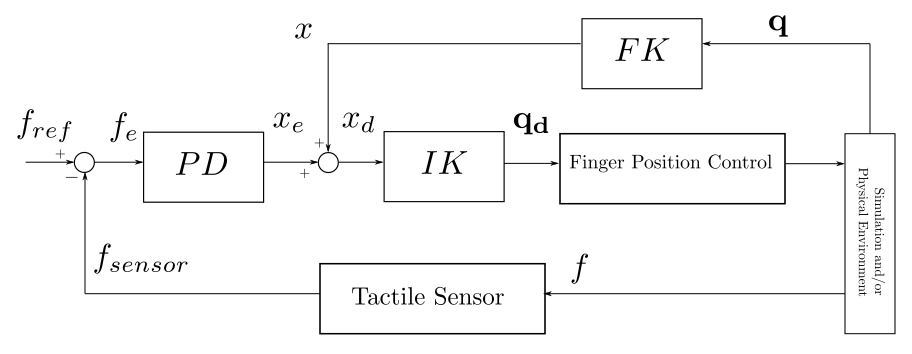
\includegraphics[width=12cm]{images/finger-force-control.png}\\
\caption{Force control on a Barrett Hand gripper finger}
\label{finger-force-control}
\end{figure}
\end{center}

To ensure a firm grasp of the surgical tool, so that it can later be more easily and precisely manipulated to do pivot surgical motions, a reference force is required to be defined. The following analysis is 
for one of the 3 fingers of the gripper and it is the same for all of them. Following the block diagram of \ref{finger-force-control}, if the actual measured force is 0, then the finger is not in contact, which means that 
there is an error in force. This force error produces a position error via a first PD controller. This position error will be positive and will be added to the current measured position and thus will make the finger move 
closer to the object. When the finger contacts for the first time the object, then the measured force is non-zero, 
but it is still less than the desired force that is required for a firm grasp. This means that there is still a force error, which again produces a positions error and again makes the finger move even closer ("squeeze") the 
object. This control loop repeats until a satisfactory contact is reached and until the desired force is exerted on the object. If the measured force is bigger than the desired value, then the force error is negative and thus
a negative position error is generated which in its turn makes the finger to move slightly away from the object, in order to reduce the exerted force. More about force control principles can be found at 
\url{http://www.osrobotics.org/osr/control/principles.html} as well as an example of force control in ROS and Gazebo at \url{http://www.osrobotics.org/osr/control/examples.html}.
\section{Simulation with the ROS framework}

\subsection{Gazebo simulation environment}

\begin{center}
\begin{figure}[H]
\centering
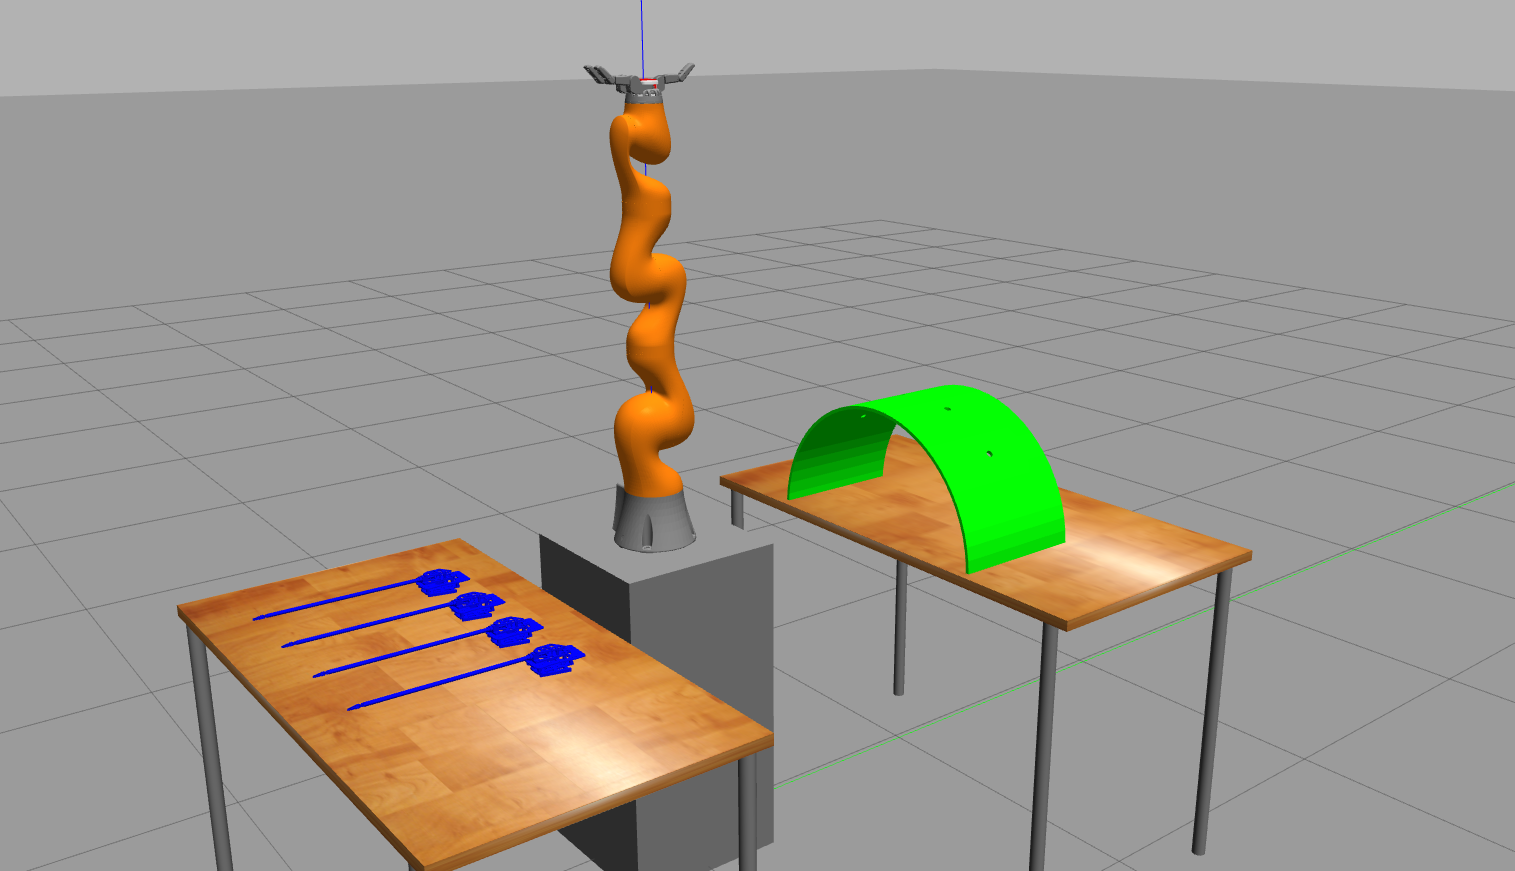
\includegraphics[width=12cm]{images/gazebo-sim1.png}\\
\caption{Simulation environment in Gazebo}
\end{figure}
\end{center}

\subsection{Visualization and Motion Planning with RViz and Moveit}

Motion Planning parameters outside of body:
\begin{itemize}
	\item Position tolerance: 50μm
	\item Orientation tolerance: 0.00005 deg
	\item Planning time: 10s
\end{itemize}

Motion Planning parameters inside of body:
\begin{itemize}
	\item Position tolerance:
	\item Orientation tolerance:
	\item Planning time
	\item End-effector interpolation step: 1mm
	\item Maximum velocity scaling factor
\end{itemize}
\chapter{Experiments and Results}

\section{Robot Planner 1: Simple MoveIt planning}

In this first experiment we are testing some simple trajectories with the surgical tool already attached to the robot arm's end effector.
The path is designed using the appropriate coordinates and orientations so that the robot begins from the home position, then visits the table with the surgical 
tools and then visits the other table on top of which the mounting dock is placed. Upon arrival at the mounting dock, the robot inserts the tool inside a hole
(we consider these holes to be a simplistic alternative to the trocars used in real operations), then executes a simple pivot motion, while the tool is still 
inserted and then the tool gets ejected from the mounting dock's hole.\\

The aim of this experiment is to test the overall behaviour of the robot inside the work space, before implementing more complex path planning algorithms.

\begin{center}
\begin{figure}[!htb]
\centering
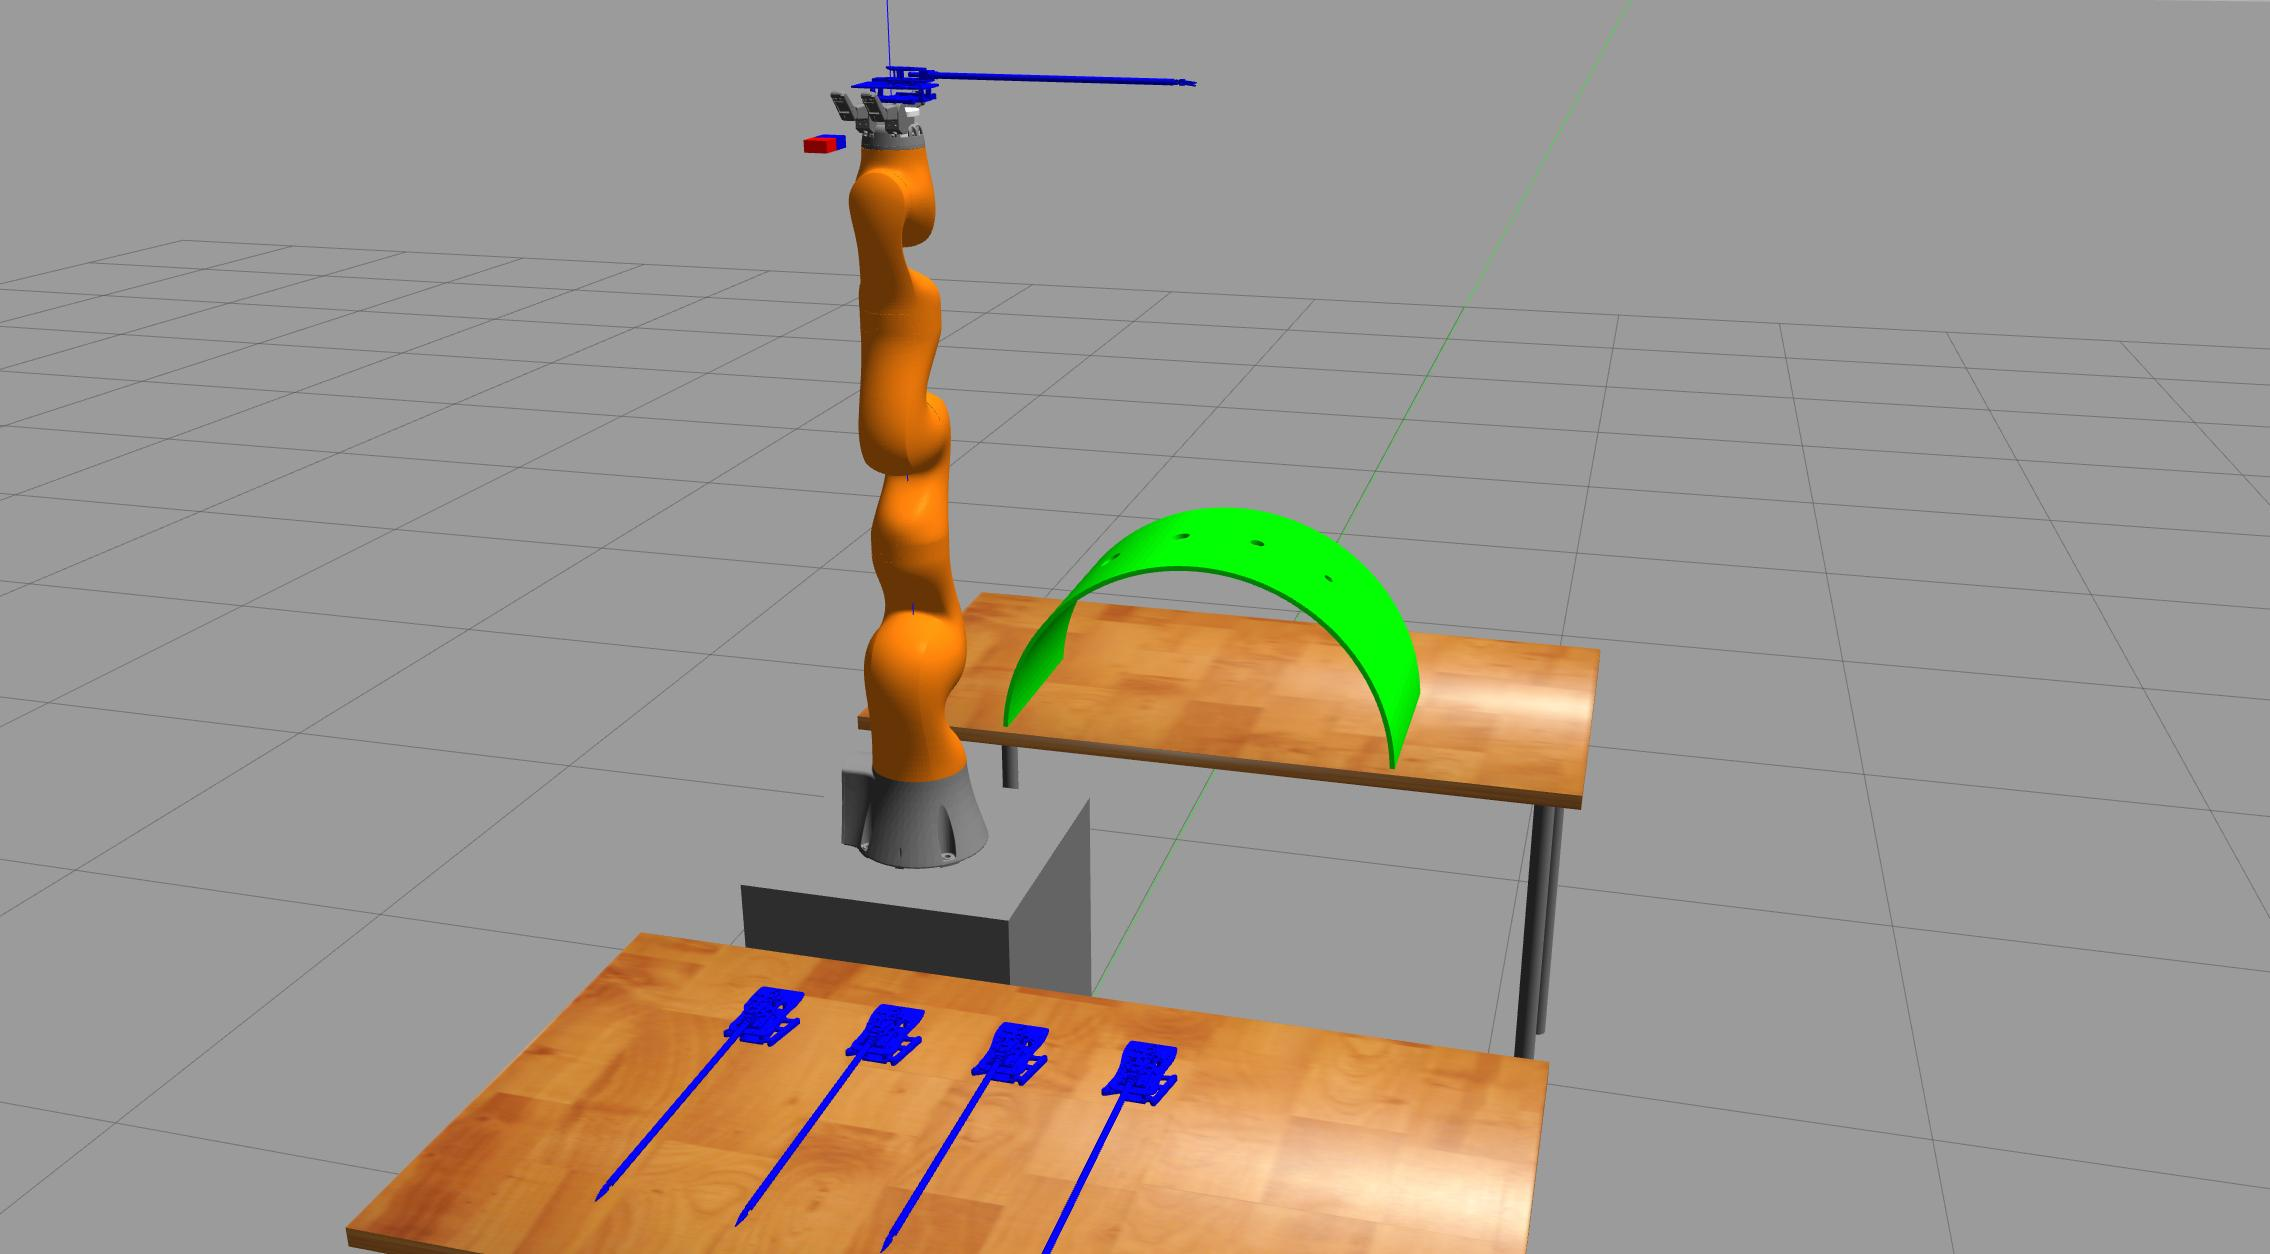
\includegraphics[width=0.3\textwidth]{images/robot_planner1/robot_planner1_1}
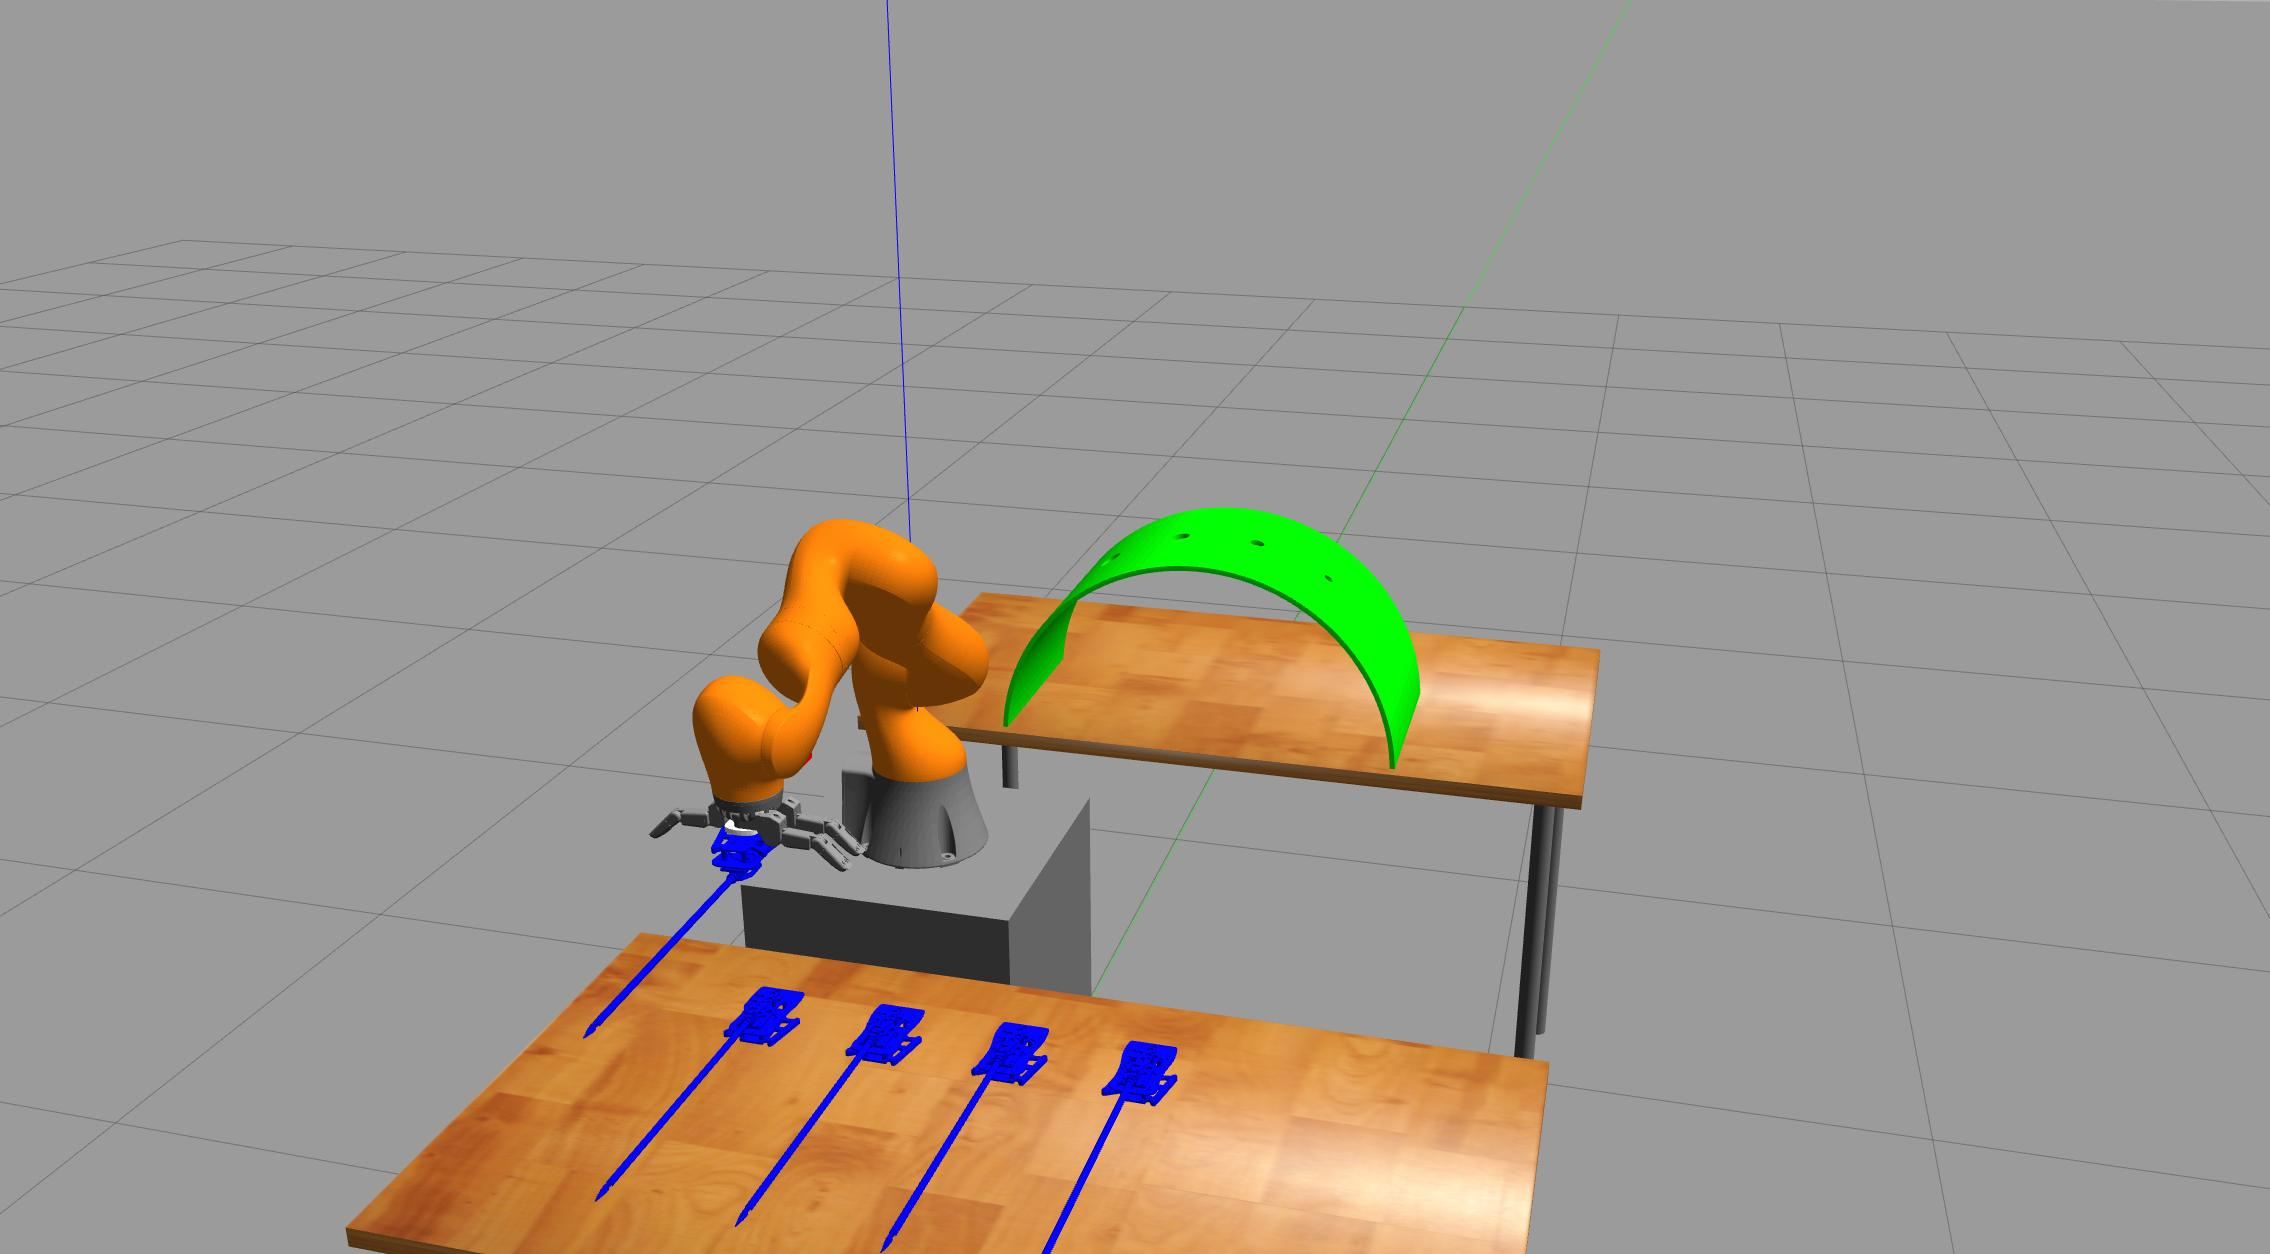
\includegraphics[width=0.3\textwidth]{images/robot_planner1/robot_planner1_2}
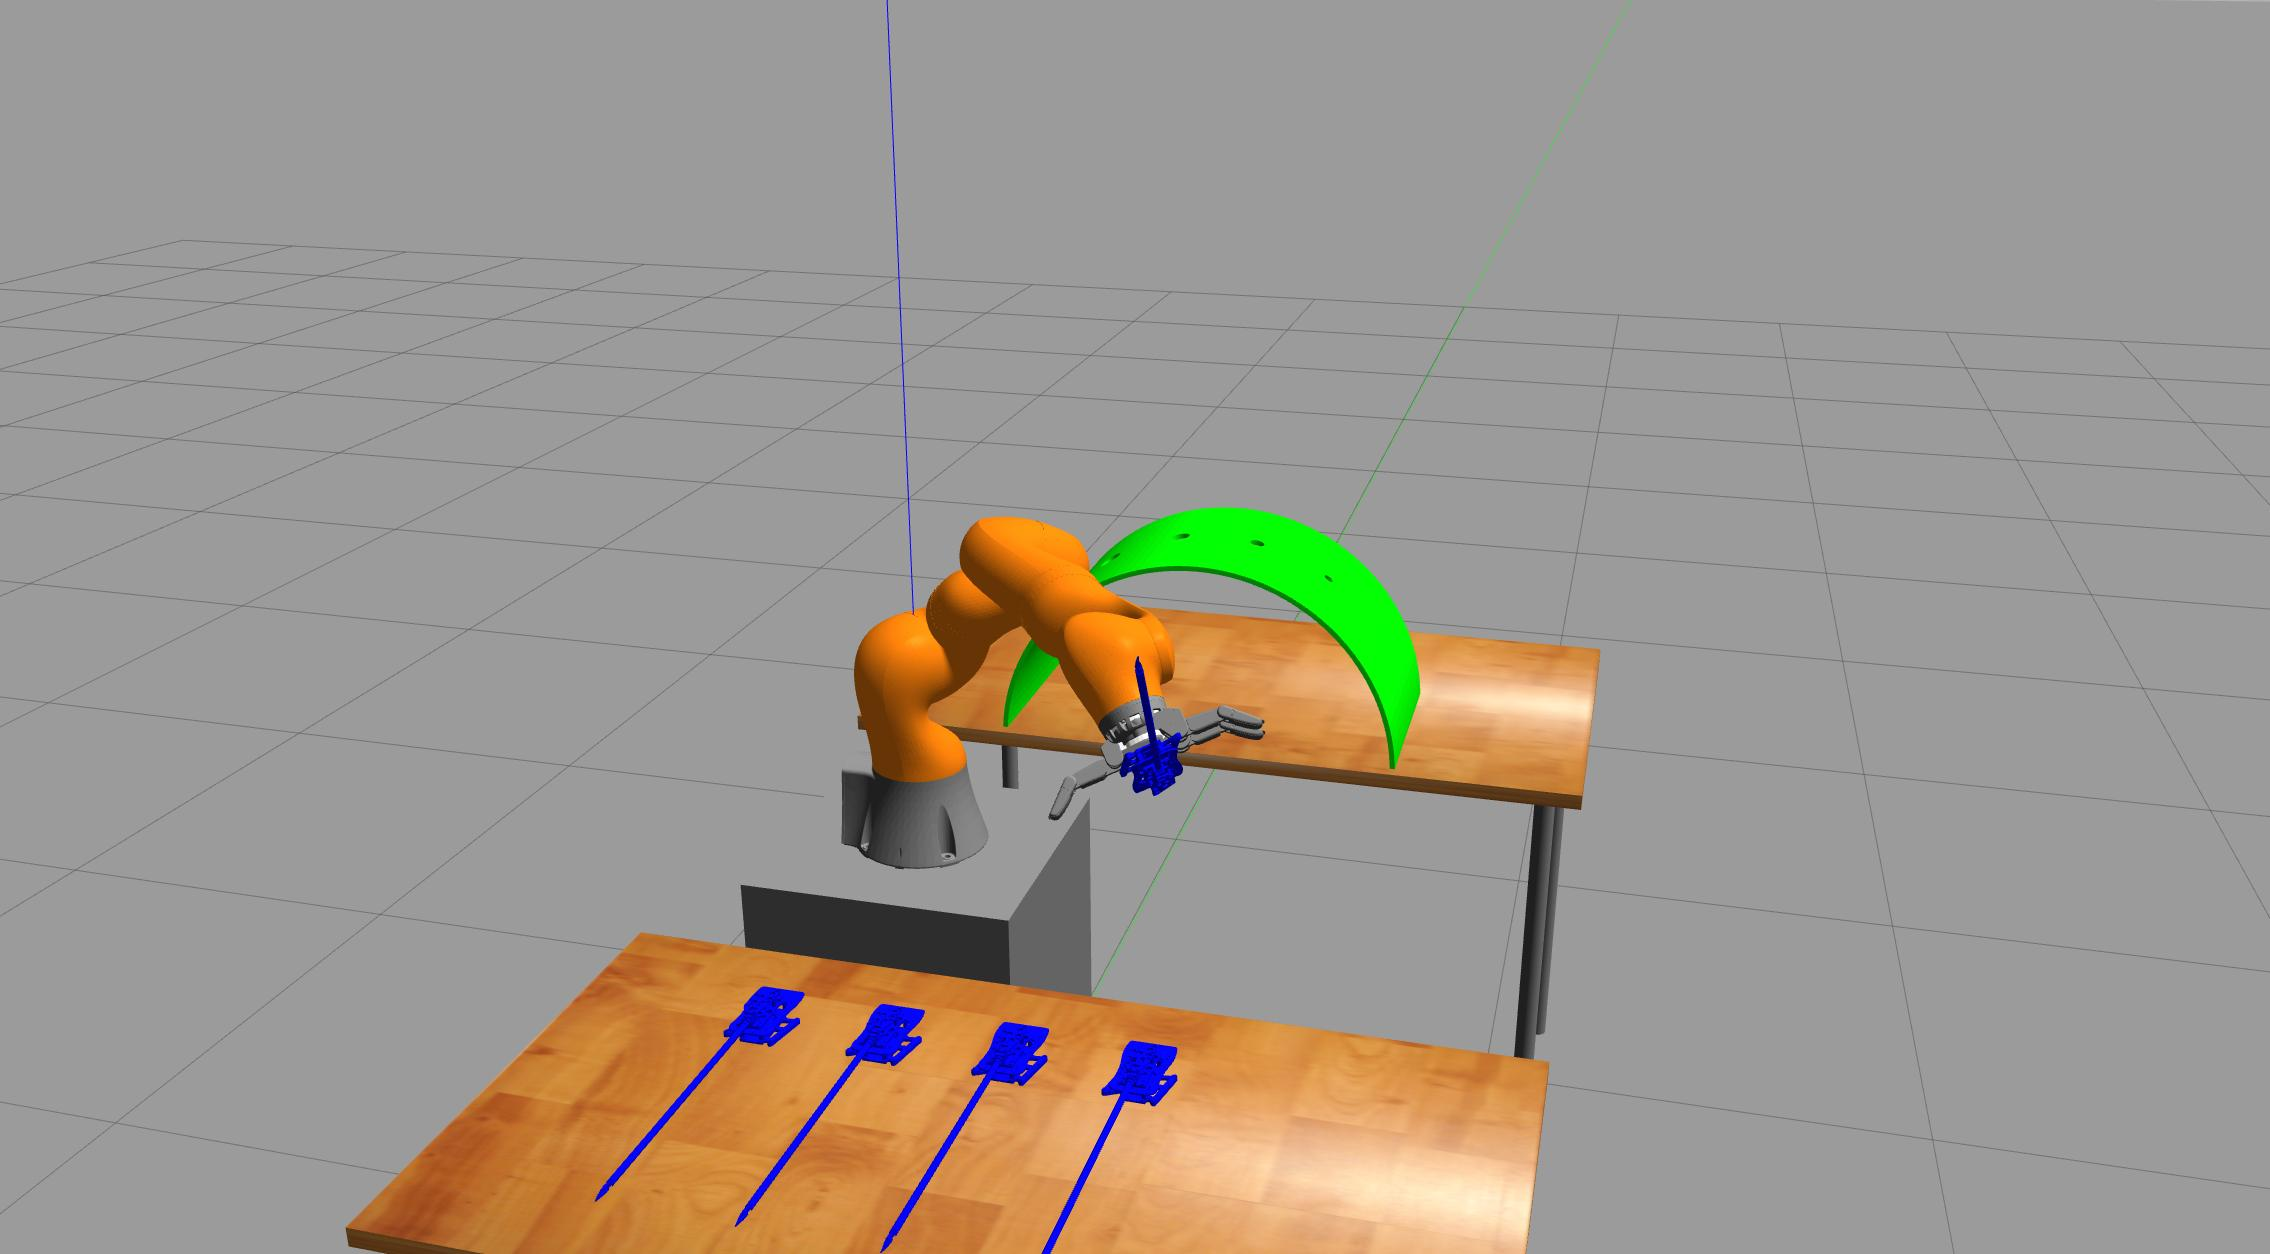
\includegraphics[width=0.3\textwidth]{images/robot_planner1/robot_planner1_3}\\
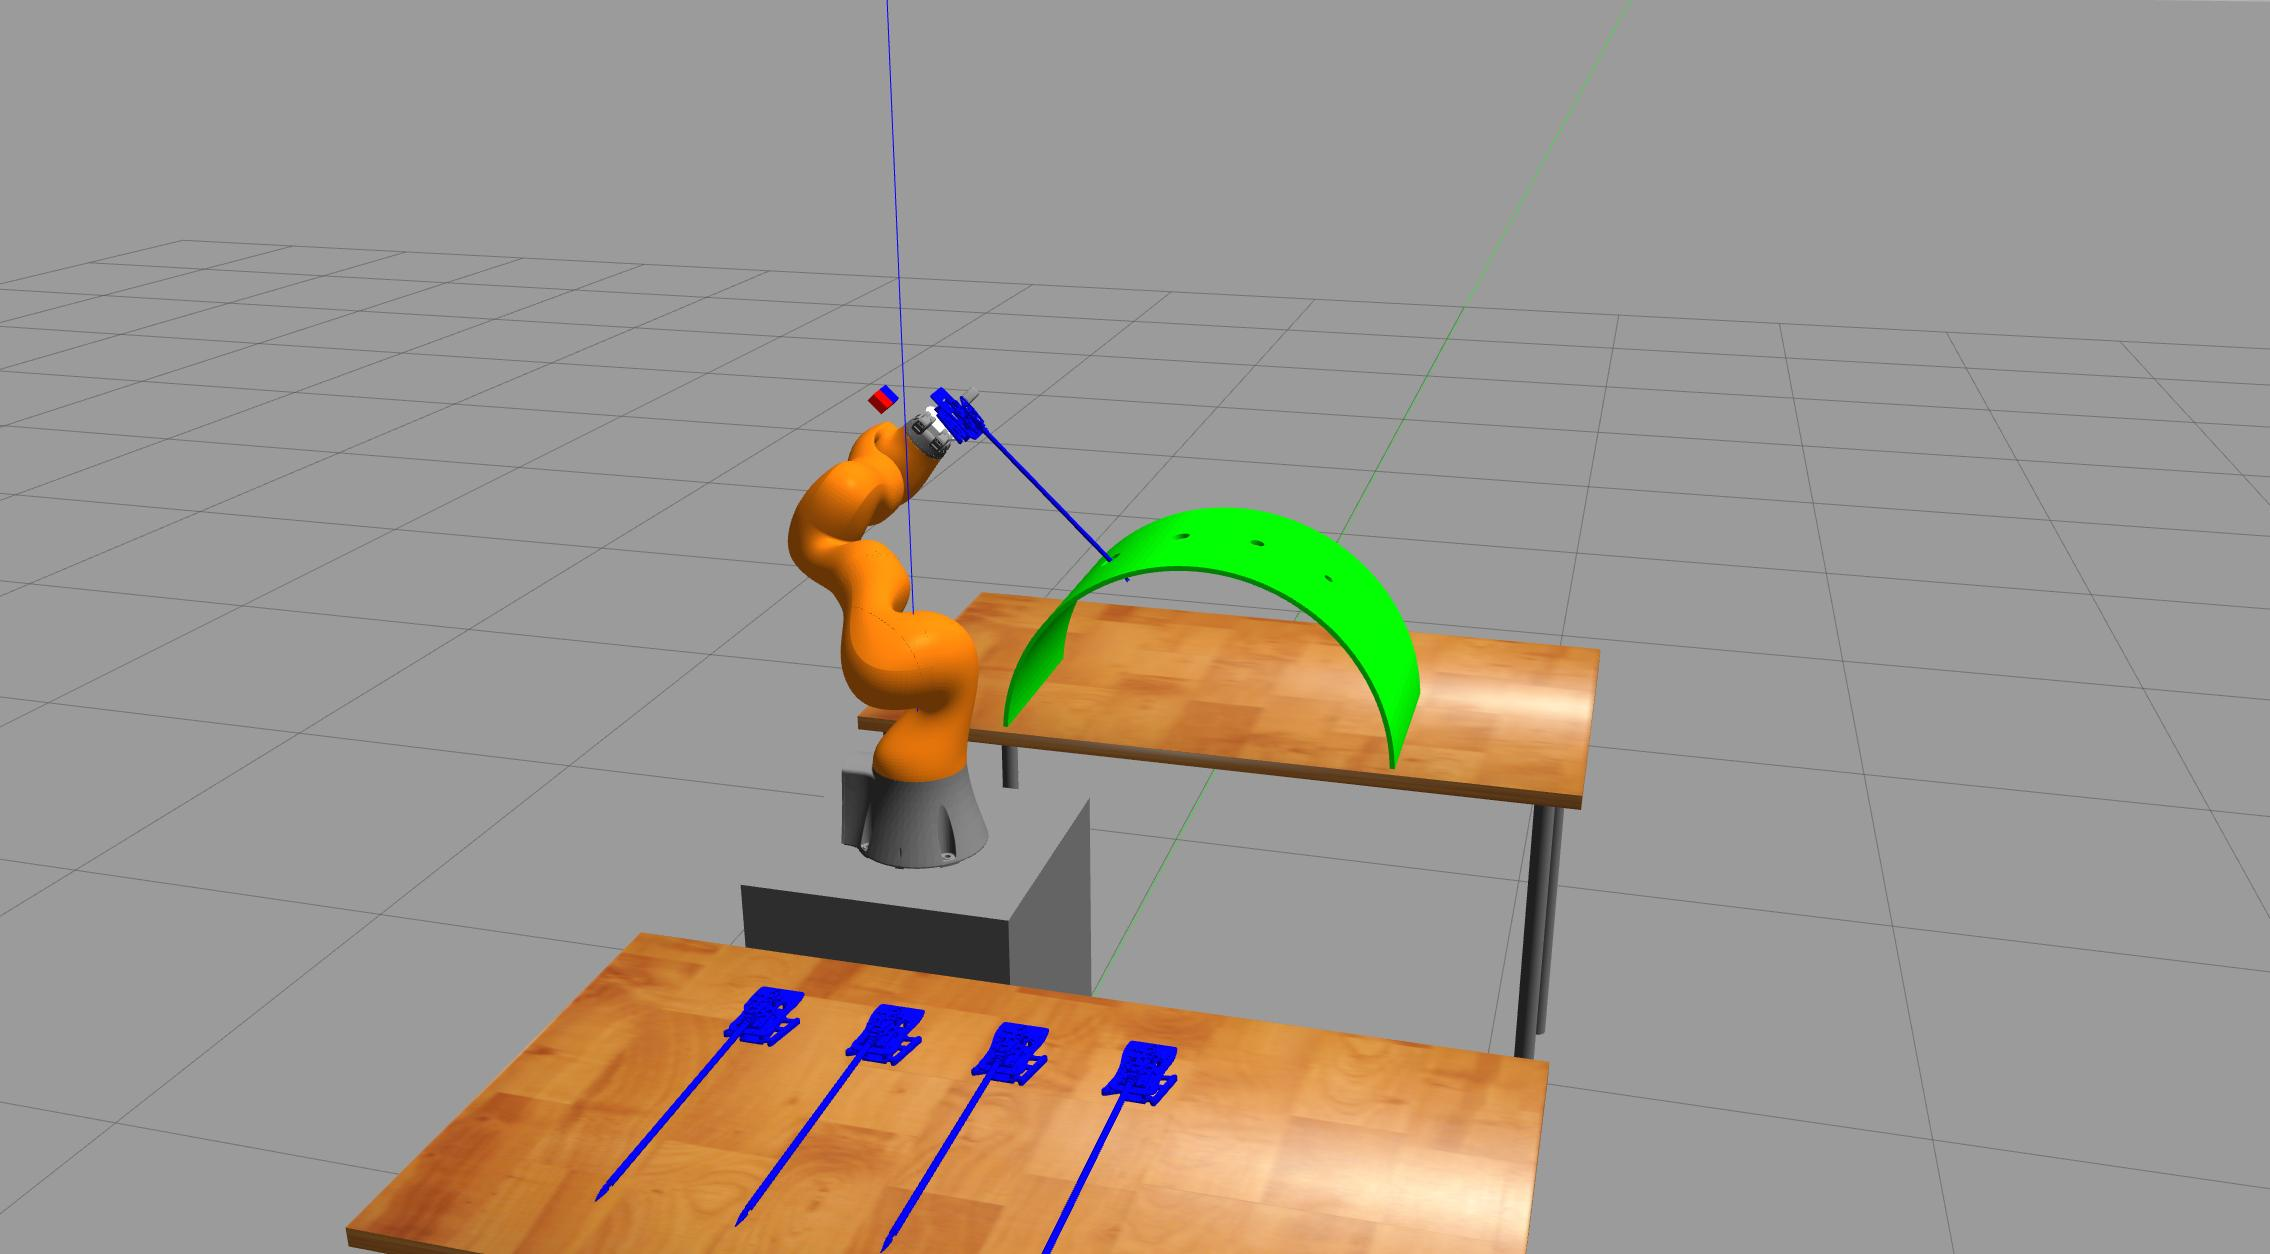
\includegraphics[width=0.3\textwidth]{images/robot_planner1/robot_planner1_4}
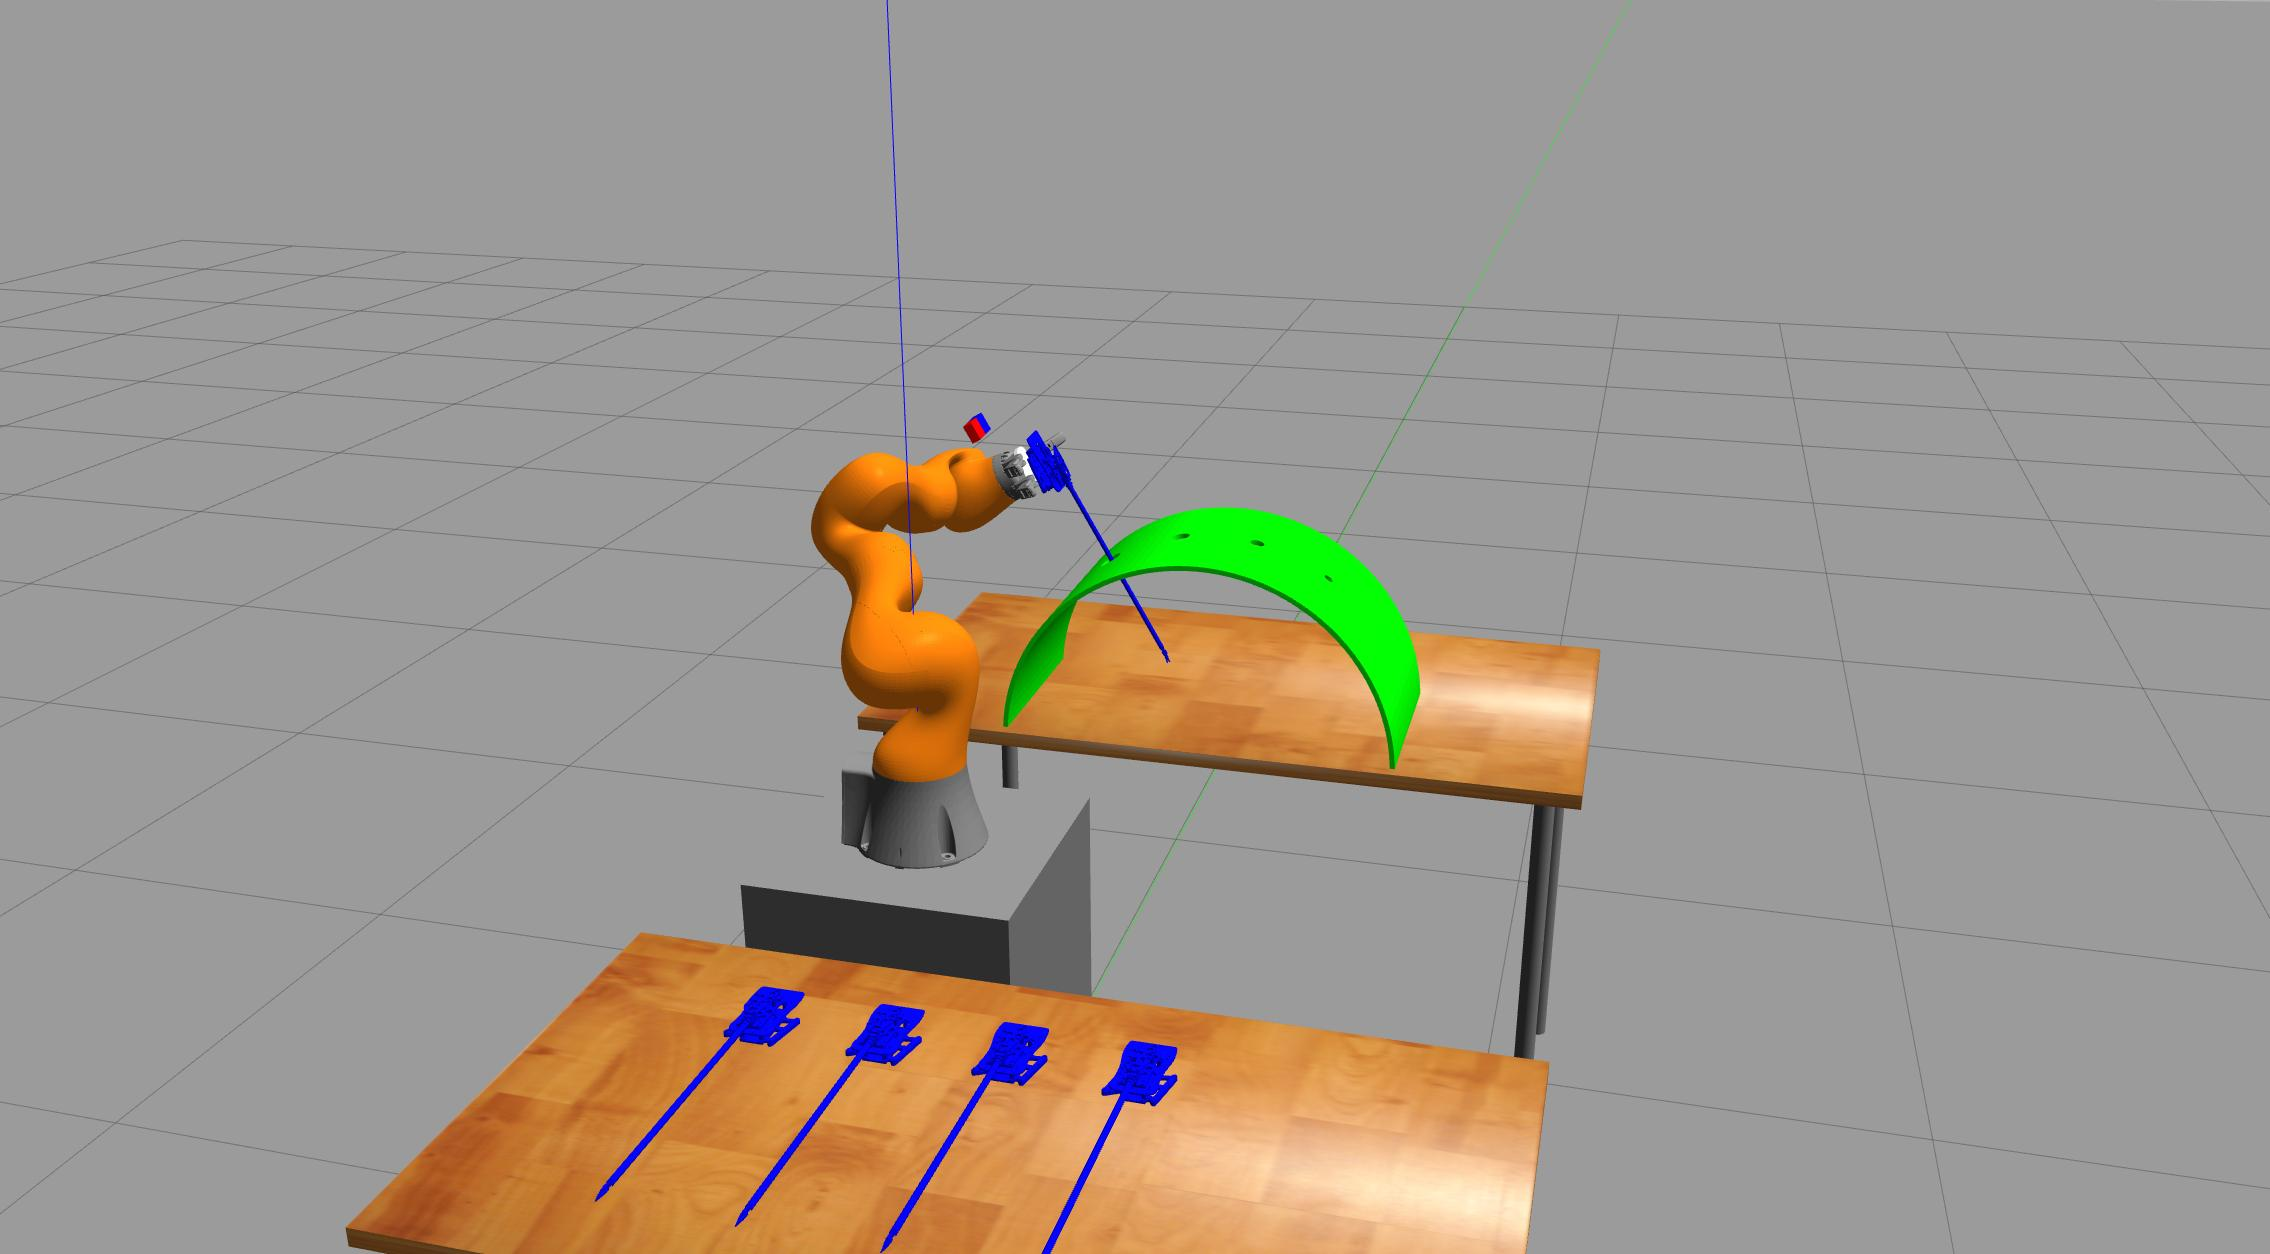
\includegraphics[width=0.3\textwidth]{images/robot_planner1/robot_planner1_5}
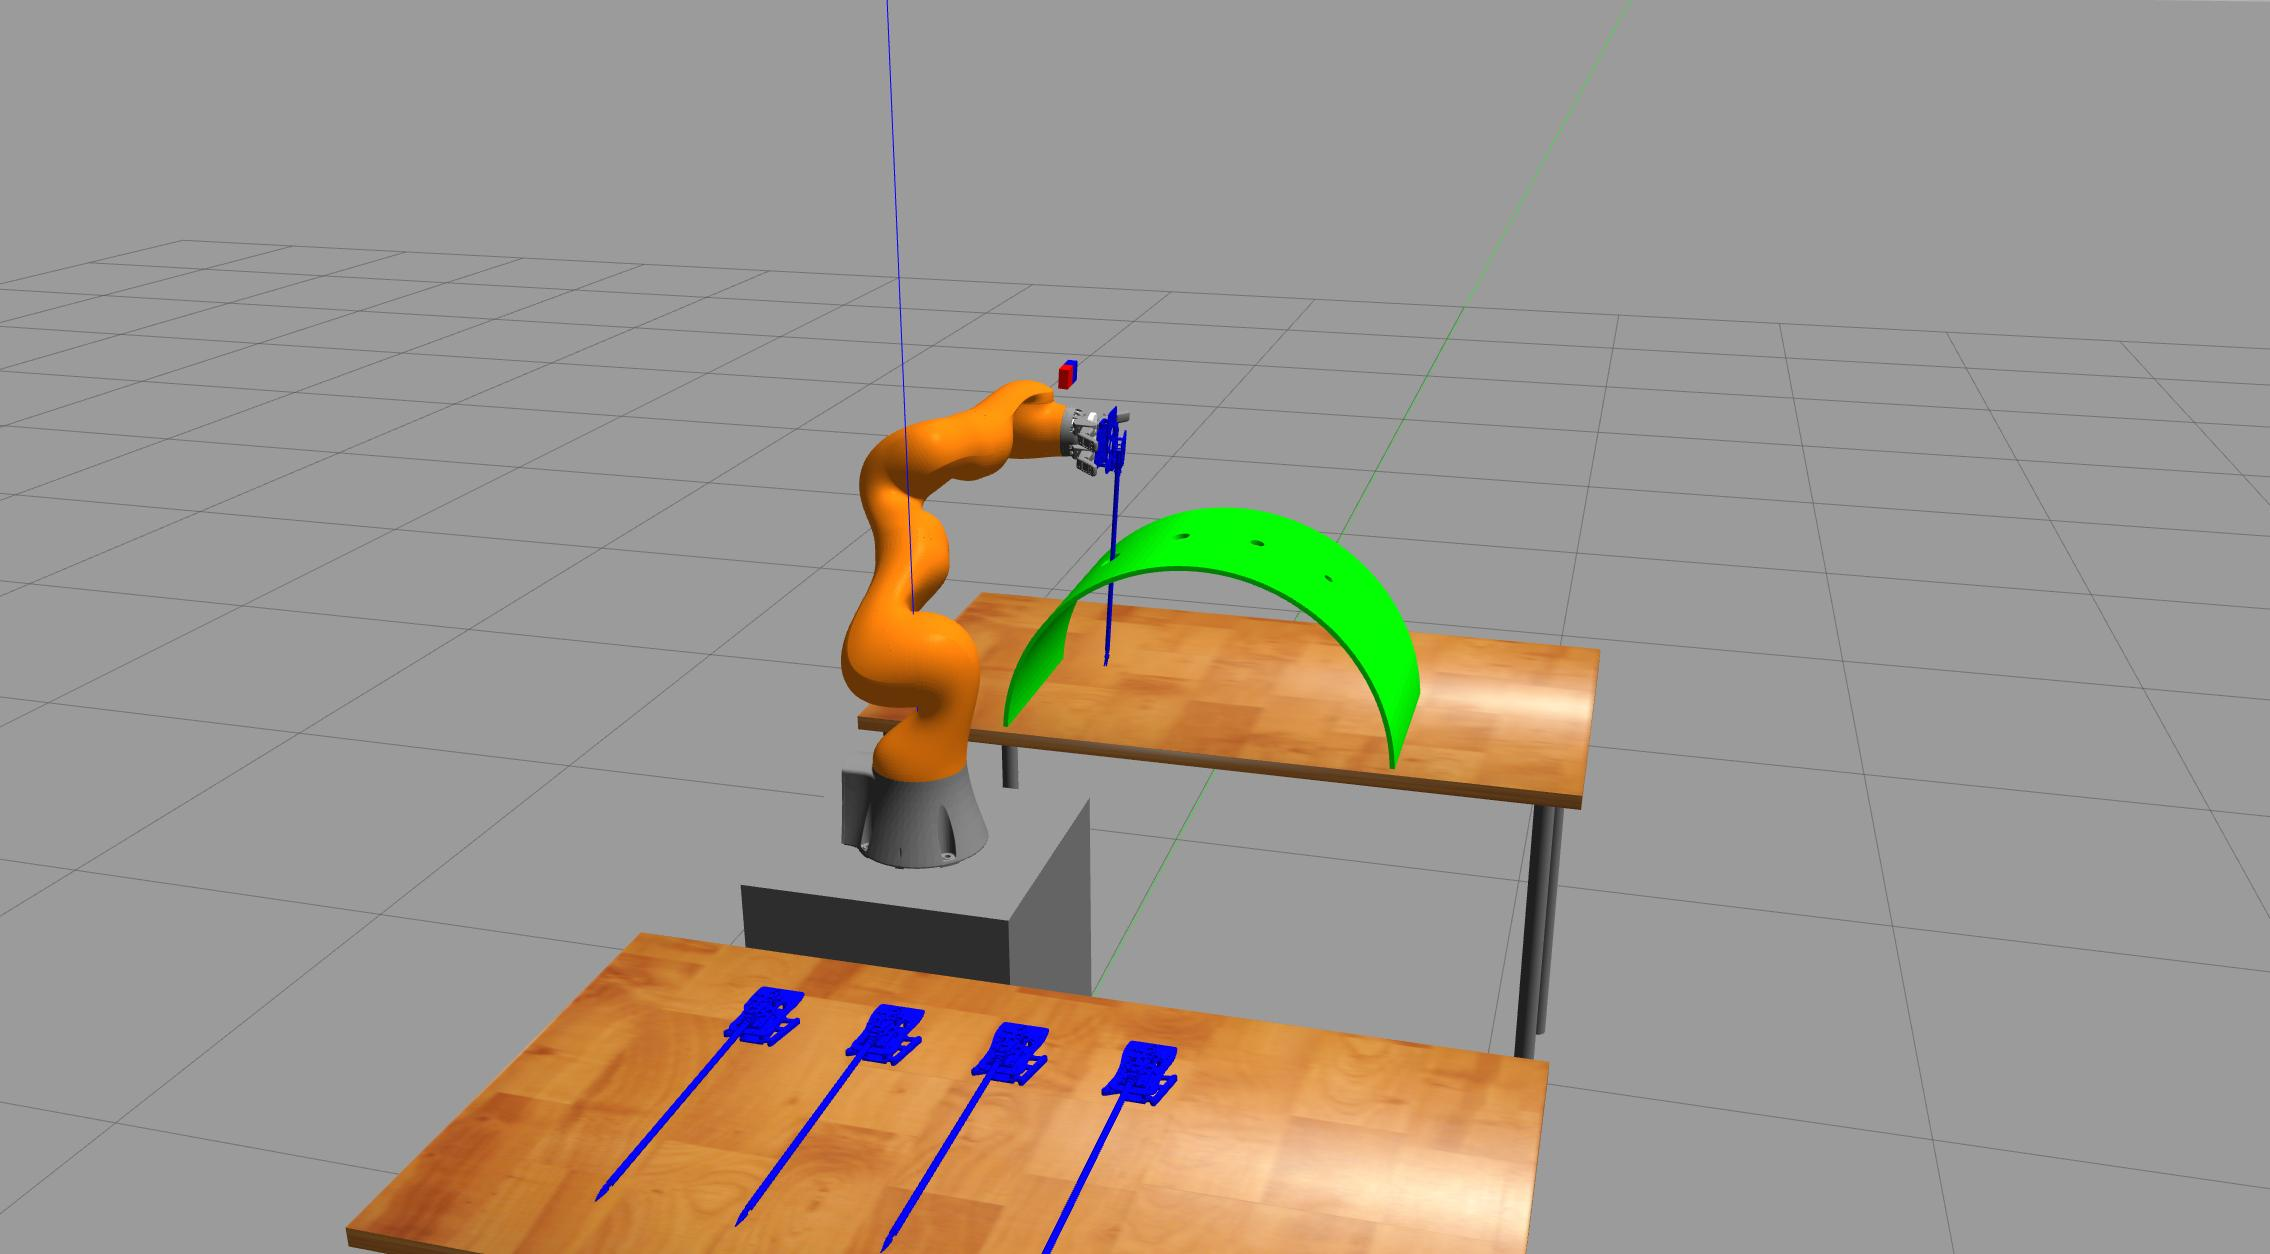
\includegraphics[width=0.3\textwidth]{images/robot_planner1/robot_planner1_6}\\
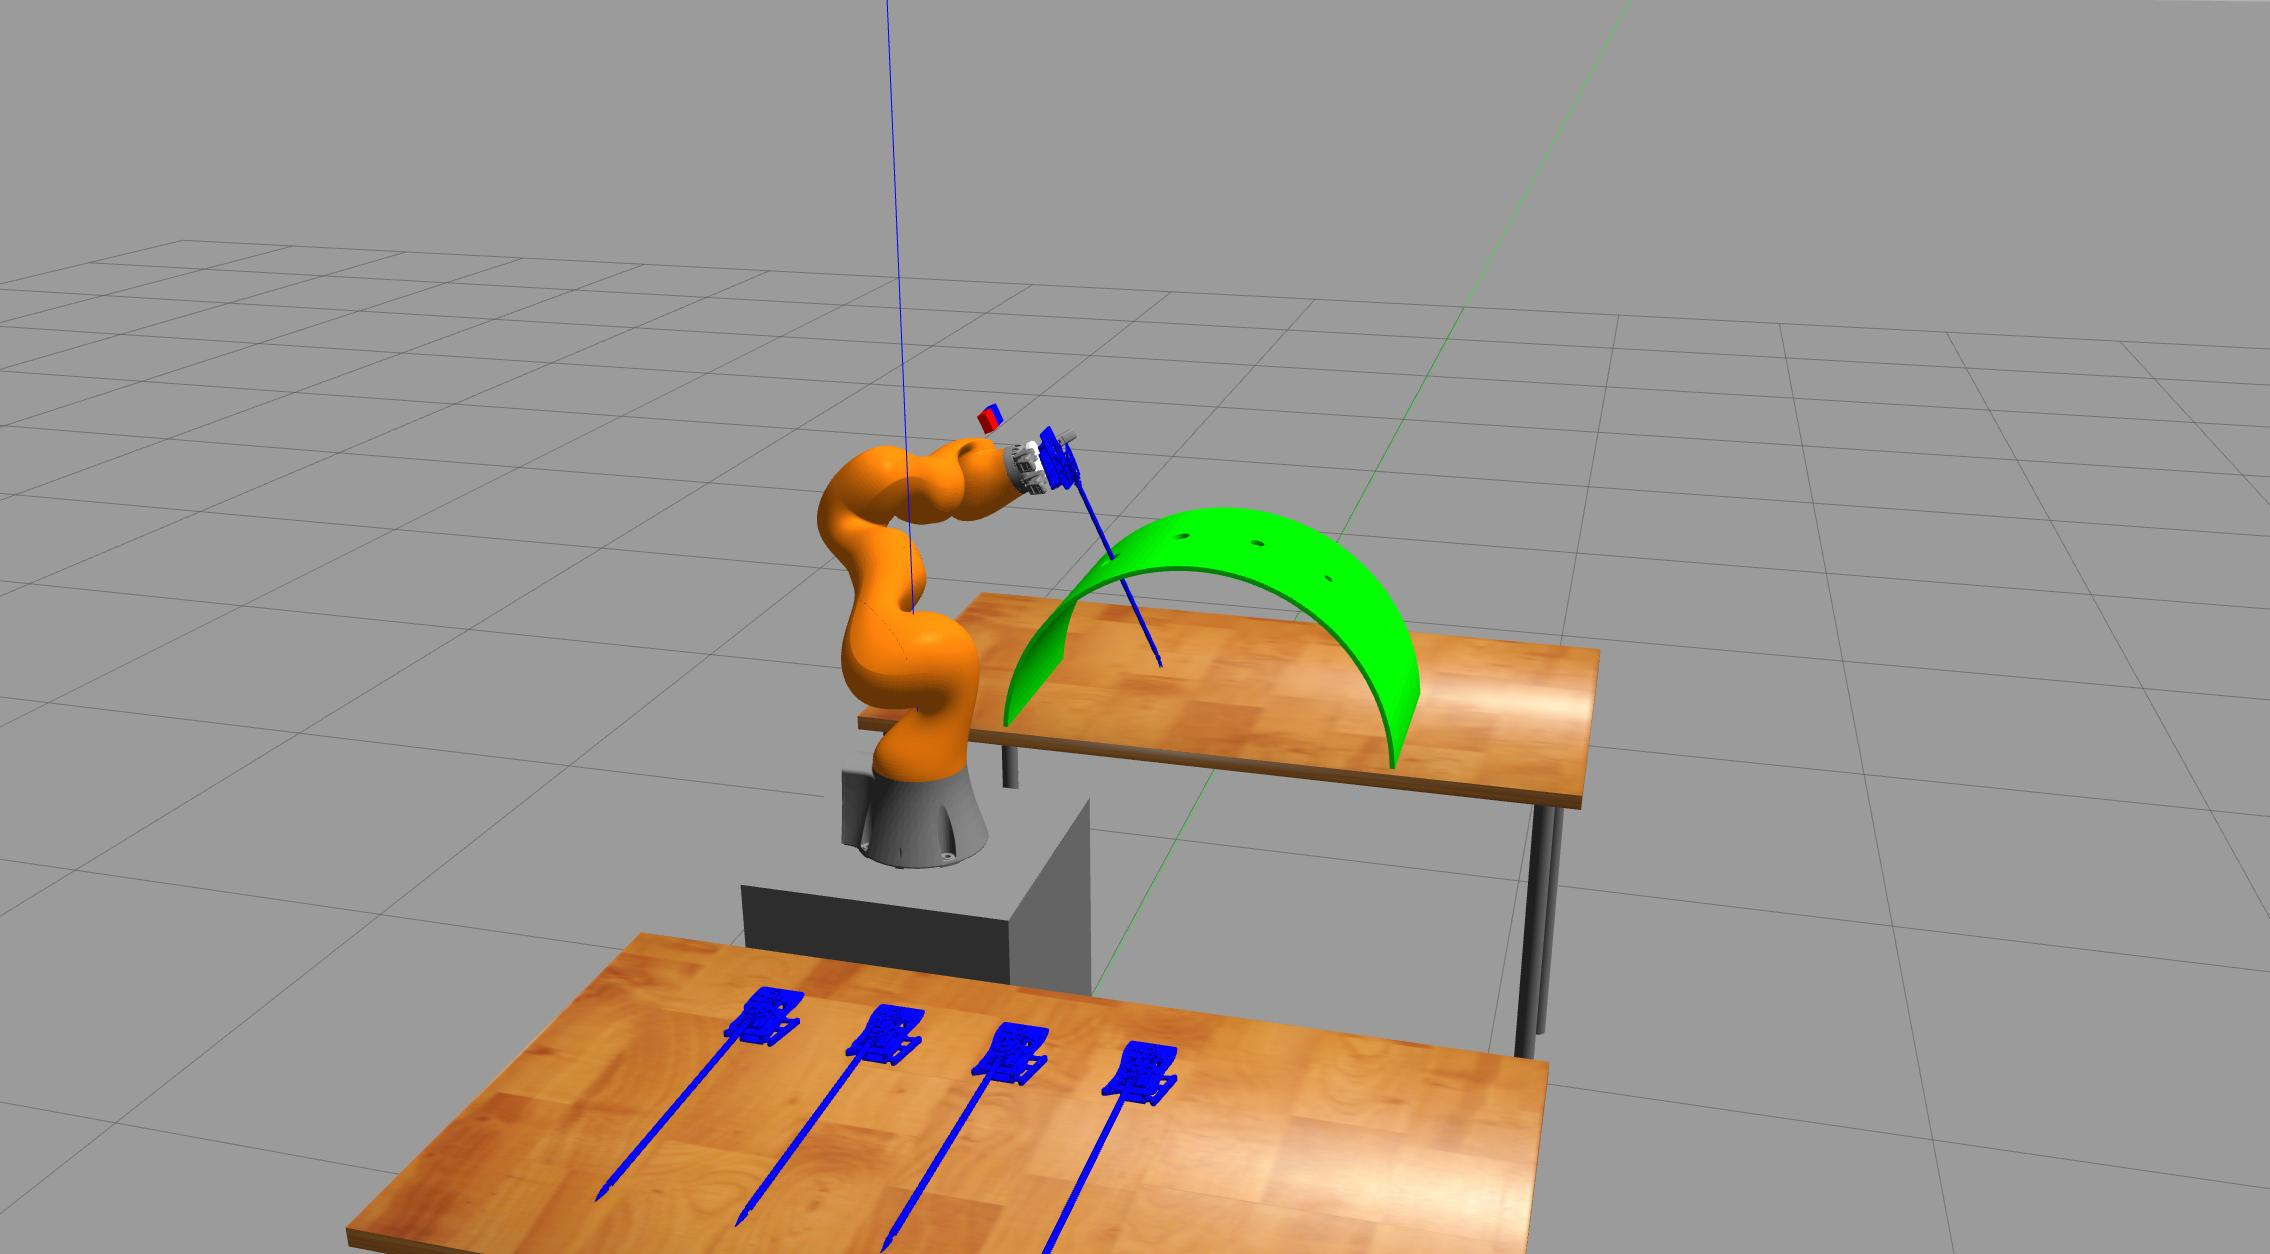
\includegraphics[width=0.3\textwidth]{images/robot_planner1/robot_planner1_7}
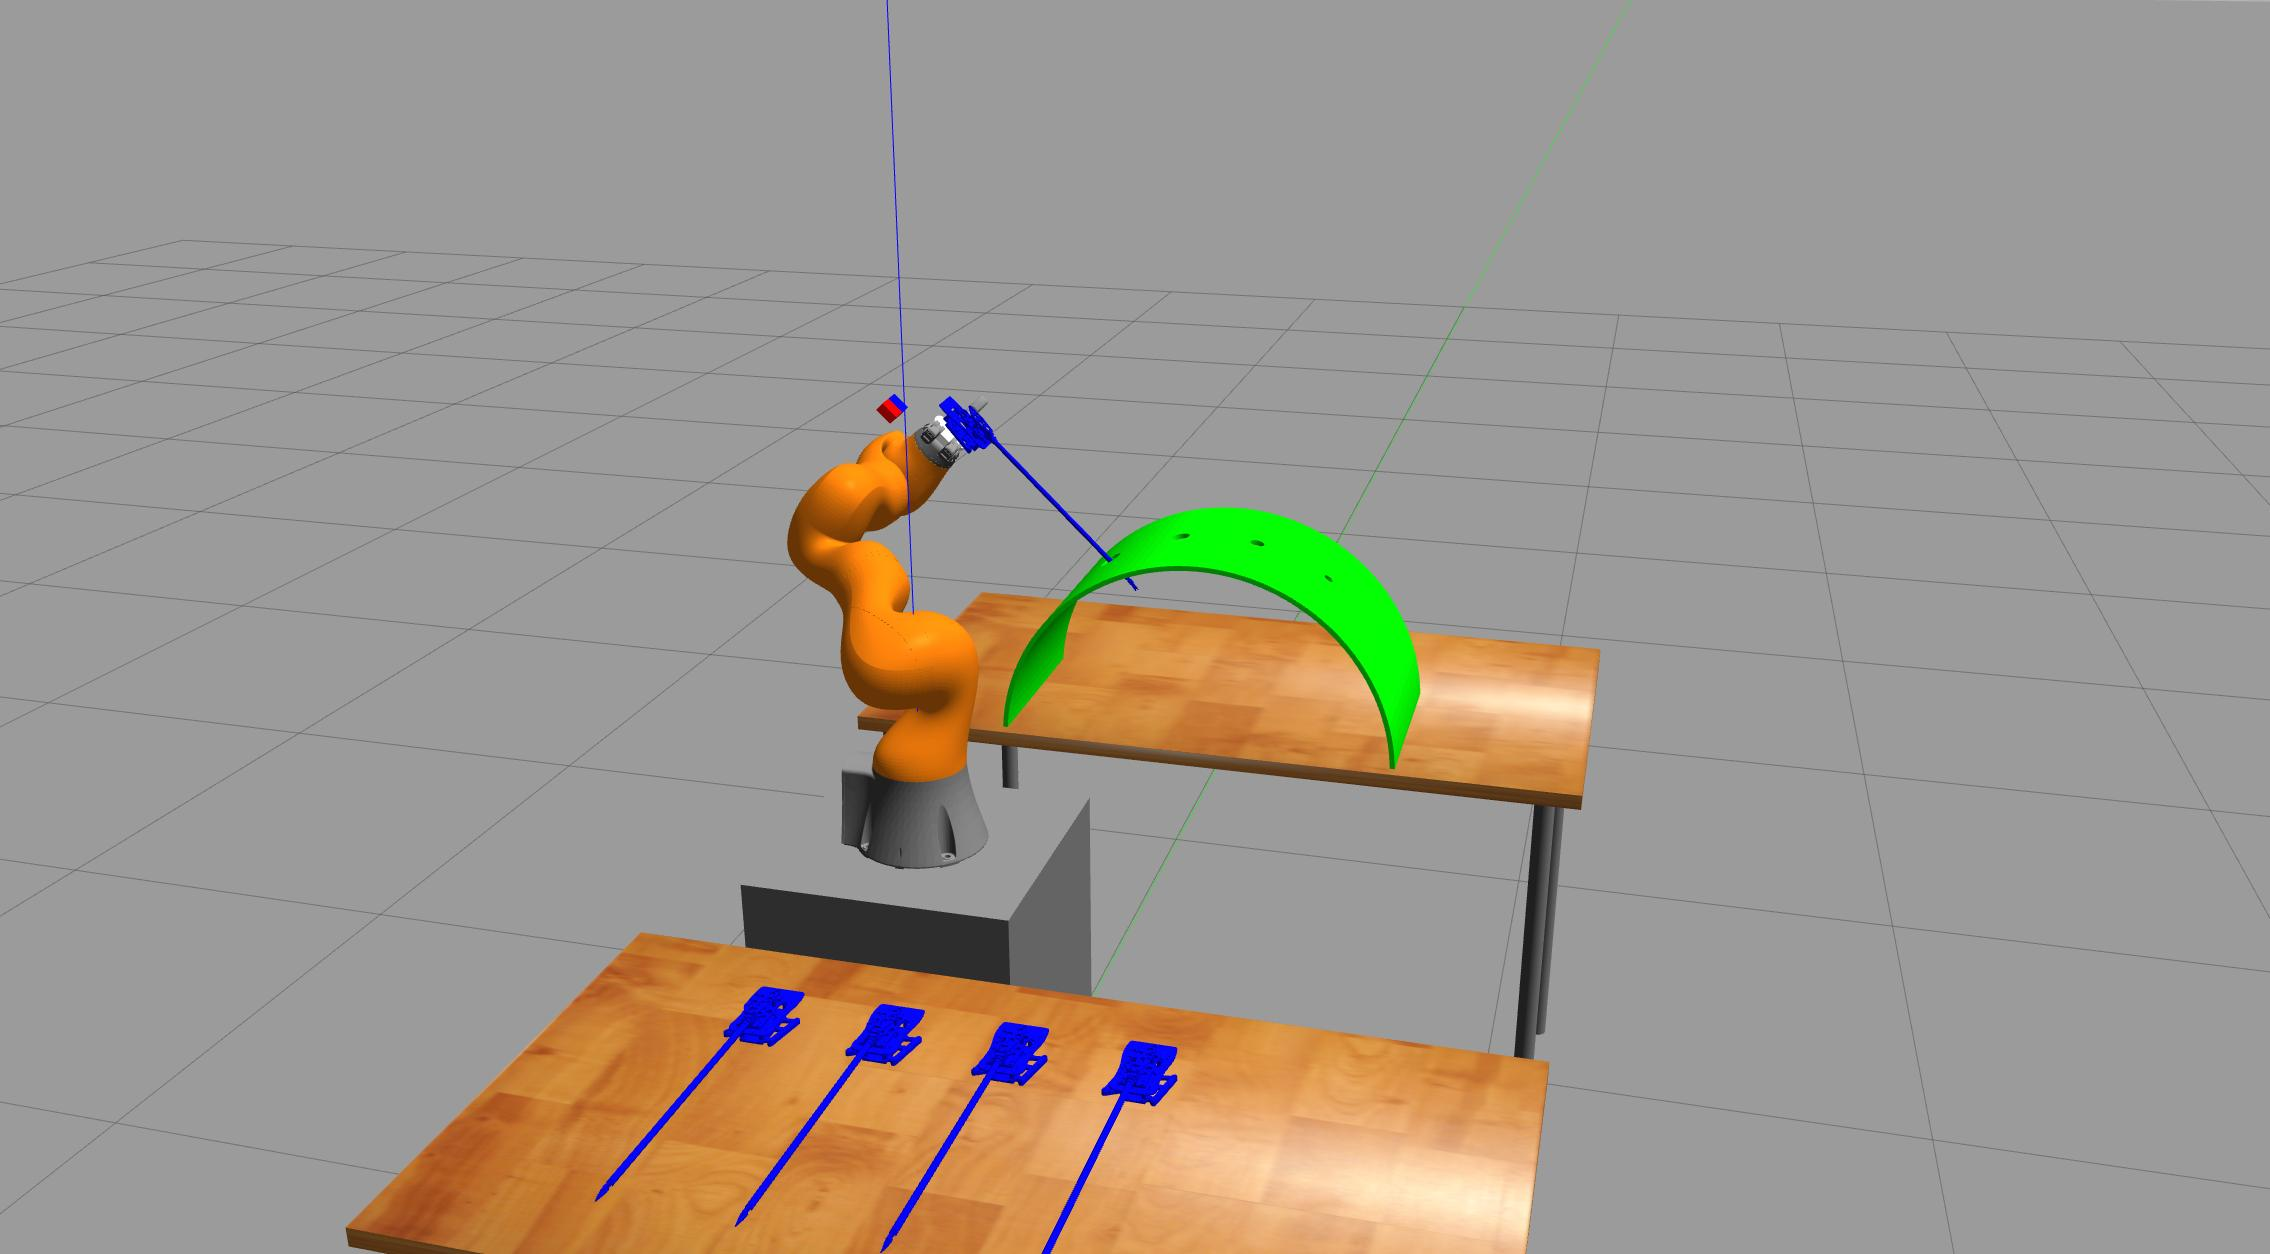
\includegraphics[width=0.3\textwidth]{images/robot_planner1/robot_planner1_8}
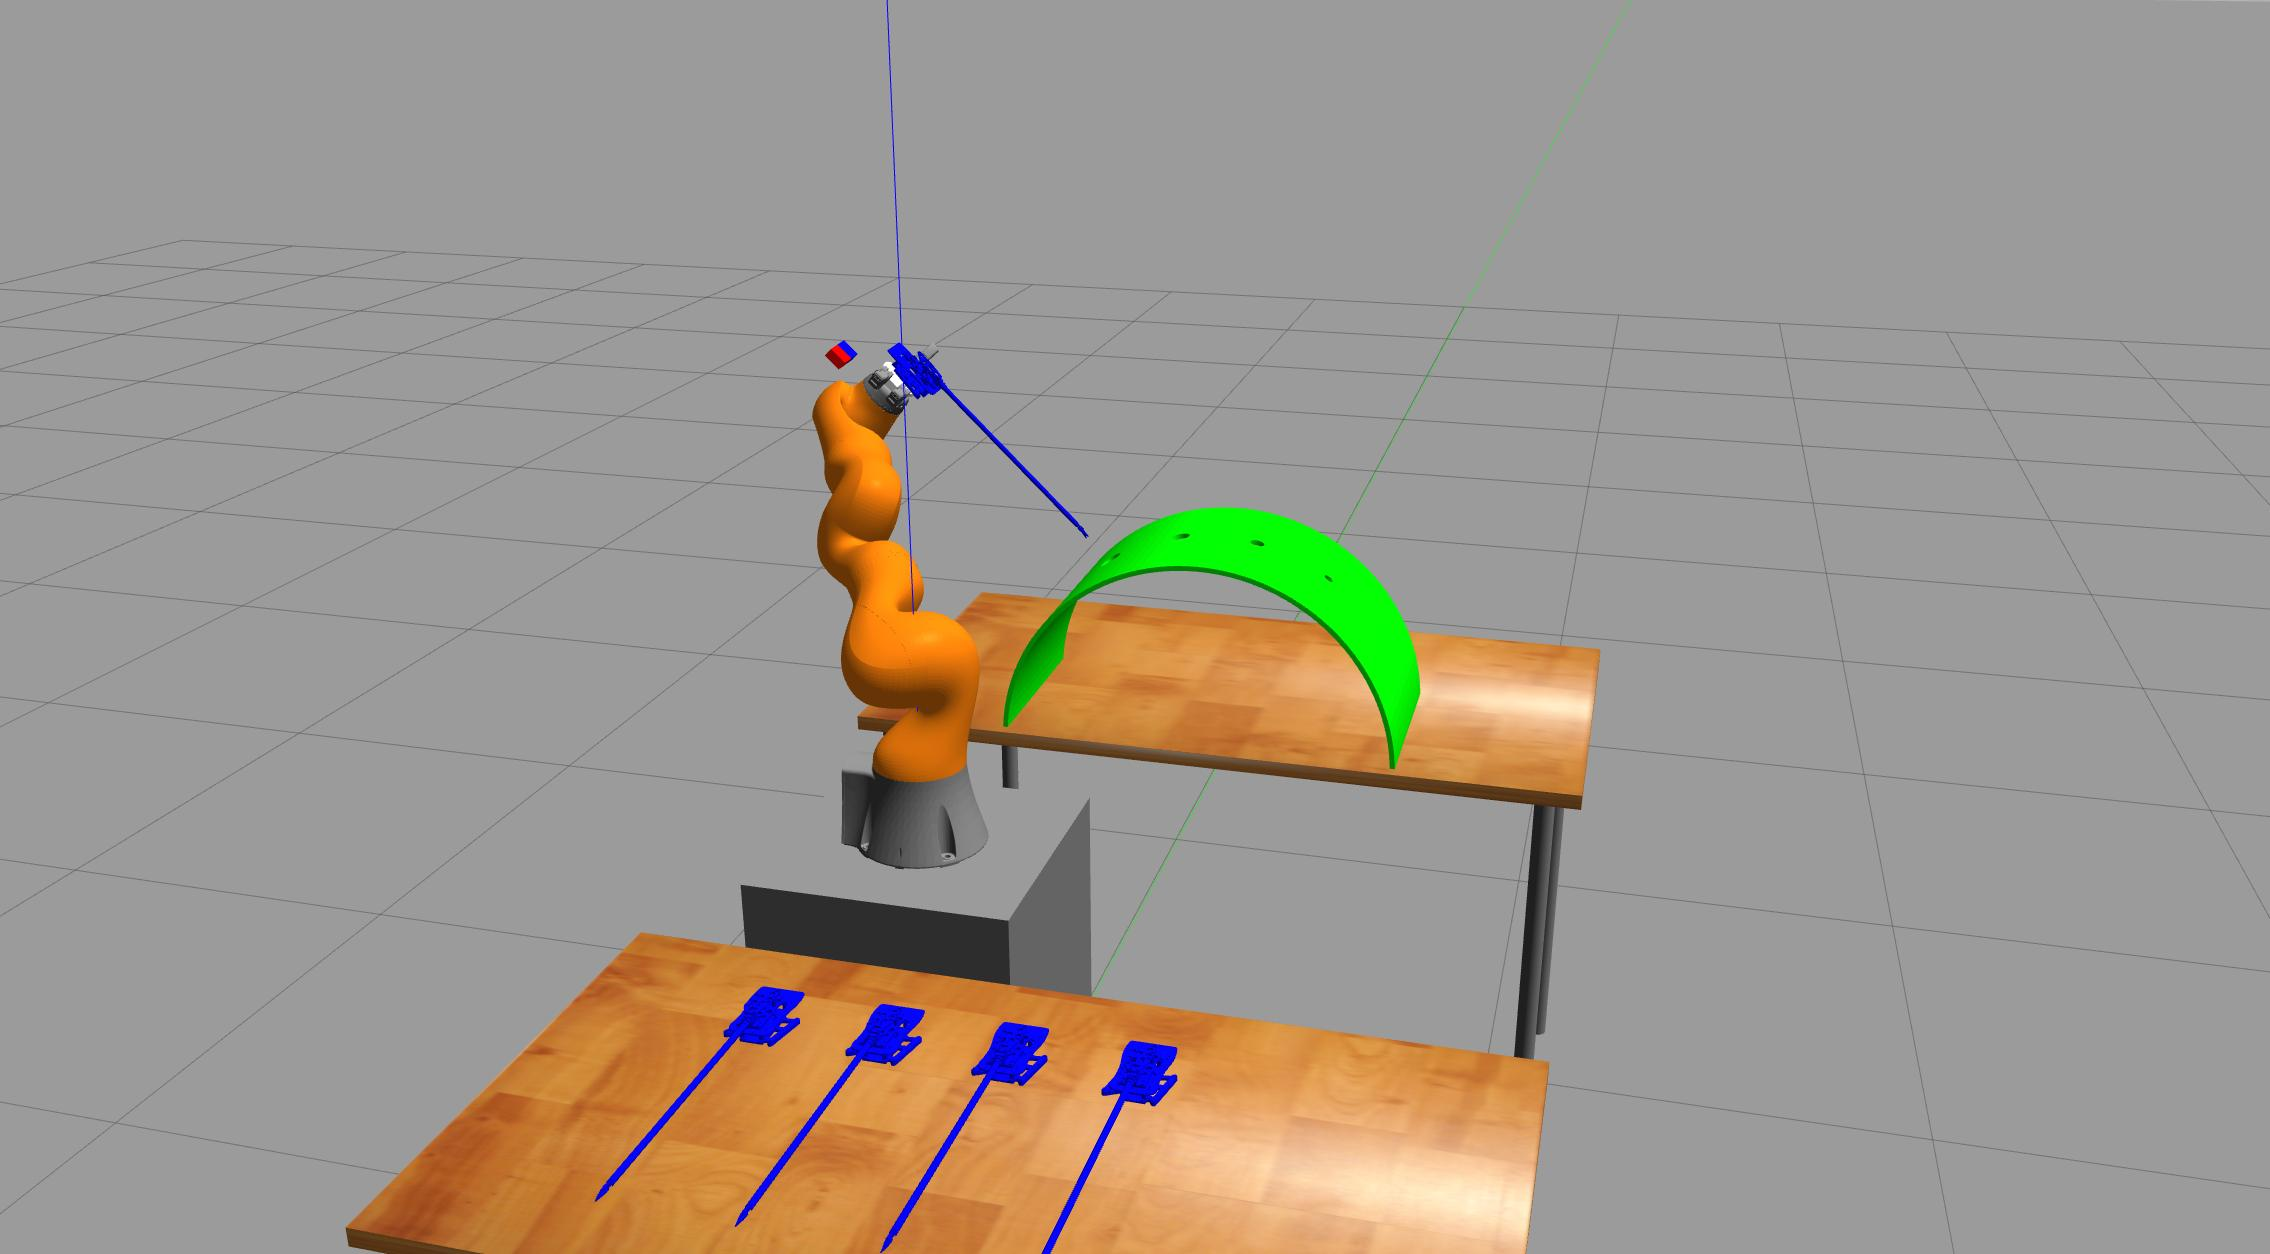
\includegraphics[width=0.3\textwidth]{images/robot_planner1/robot_planner1_9}\\
\caption{Experiment 1:}
\end{figure}
\end{center}

% Robot Planner 1 with RRTConnect
\begin{table}[H]
\centering
\begin{tabular}{|p{2cm}|c|p{2cm}|p{2cm}|p{2cm}|}
\hline
Robot Planner 1           & \multicolumn{4}{c}{\textbf{RRTConnect}}                                                                                                 \vline \\
\hline
                          & \multicolumn{4}{c}{\textbf{Fake tool picking trajectory}}                     \vline \\
\hline
Experiment                & Approach planning time & Execution status & Move away planning time & Execution status  \\
\hline
1 &	0.060402 &	1 &	0.144881 &	1 \\
2 &	0.06053 &	1 &	0.058341 &	1 \\
3 &	0.064706 &	1 &	0.060981 &	1 \\
4 &	0.059789 &	1 &	0.119351 &	1 \\
5 &	0.164789 &	1 &	0.330373 &	1 \\
6 &	0.147037 &	1 &	0.289805 &	1 \\
7 &	0.18233 &	1 &	0.093362 &	1 \\
8 &	0.054469 &	1 &	0.062209 &	1 \\
9 &	0.05313 &	1 &	0.409191 &	1 \\
10 &	0.105909 &	1 &	0.307963 &	1 \\
\hline
\textbf{Average} & 	0.0953091 &	1	& 0.1876457	& 1 \\
\hline
                          & \multicolumn{4}{c}{\textbf{Insertion \& Pivot trajectories}}                     \vline \\
\hline
Experiment                & Insertion planning time & Execution status & Pivot planning time & Execution status  \\
\hline
1	& 0.216565	& 1	& 3.639193	& 1 \\
2	& 0.057143	& 1	& 0.057187	& 1 \\
3	& 0.073242	& 1	& 0.072451	& 1 \\
4	& 0.056255	& 1	& 0.068156	& 1 \\
5	& 0.16178	& 1	& 0.150123	& 1 \\
6	& 0.071426	& 1	& 0.065059	& 1 \\
7	& 0.155125	& 1	& -	& 0 \\
8	& 0.315921	& 1	& 0.194663	& 1 \\
9	& 0.127381	& 1	& 0.19026	& 1 \\
10	& 0.396182	& 1	& 0.075866	& 1 \\
\hline
\textbf{Average} & 	0.163102 & 1	& 0.5014398 &	0.9 \\
\hline
                          & \multicolumn{4}{c}{\textbf{Reverse pivot \& retraction trajectories}}                     \vline \\
\hline
Experiment                & Reverse pivot planning time & Execution status & retraction planning time & Execution status  \\
\hline
1 & 2.419514	& 1	& 2.388166	& 1 \\
2 & 1.386188	& 1	& 2.874223	& 0 \\
3 & -	& 0	& 5.106926	& 1 \\
4 & 5.466561	& 1	& 4.562506	& 1 \\
5 & 5.62329	& 1	& 5.587679	& 1 \\
6 & 5.488728	& 0	& -	& 0 \\
7 & -	& 0	& -	& 0 \\
8 & -	& 0	& -	& 0 \\
9 & 5.291442	& 1	& 5.096234	& 1 \\
10 & 5.381595	& 1	& 5.576362	& 1 \\
\hline
\textbf{Average} & 	4.436760	& 0.6	& 4.456014	& 0.6 \\
\hline
\end{tabular}
\caption{Time results for robot planner 1 using the RRTConnect path planner algorithm. Planning time is the sum of solution time and path simplification time. Execution status is 
1 for success and 0 for failure. Parameters: tolerances: 0.000005, max planning time: 5 seconds, replanning: true, max planning attempts: 6. Experiments start from home position.}
\label{robot-planner1-rrtconnect-data}
\end{table}


% Robot Planner 1 with RRT*
\begin{table}[H]
\centering
\begin{tabular}{|p{2cm}|c|p{2cm}|p{2cm}|p{2cm}|}
\hline
Robot Planner 1           & \multicolumn{4}{c}{\textbf{RRT*}}                                                                                                 \vline \\
\hline
                          & \multicolumn{4}{c}{\textbf{Fake tool picking trajectory}}                     \vline \\
\hline
Experiment                & Approach planning time & Execution status & Move away planning time & Execution status  \\
\hline
1	& 5.096772	& 1	& 5.023175	& 1 \\
2	& 5.015857	& 1	& 5.034447	& 1 \\
3	& 5.01843	& 1	& 5.101766	& 1 \\
4	& 5.074703	& 1	& 5.089464	& 1 \\
5	& 5.019108	& 1	& 5.056875	& 1 \\
6	& 5.011631	& 1	& 5.217069	& 1 \\
7	& 5.119638	& 1	& 5.027692	& 1 \\
8	& 5.121159	& 1	& 5.040244	& 1 \\
9	& 5.12812	& 1	& 5.098381	& 1 \\
10	& 5.343964	& 1	& 5.374314	& 1 \\
\hline
\textbf{Average} & 	5.0949382	& 1	& 5.1063427	& 1 \\
\hline
                          & \multicolumn{4}{c}{\textbf{Insertion \& Pivot trajectories}}                     \vline \\
\hline
Experiment                & Insertion planning time & Execution status & Pivot planning time & Execution status  \\
\hline
1 & 5.200983  & 1 &  5.044568 &  1 \\
2 & 5.009846  & 1 &  -  &  0 \\
3 & 5.064216  & 1 &  5.085314 &  1 \\
4 & 5.145115  & 1 &  5.059245 &  1 \\
5 & 5.019322  & 1 &  5.173925 &  1 \\
6 & 5.015804  & 1 &  -  &  0 \\
7 & 5.033637  & 1 &  -  &  0 \\
8 & 5.159212  & 1 &  5.100395 &  1 \\
9 & 5.134356  & 1 &  5.081432 &  1 \\
10  & 5.052 & 0  & - &  0 \\
\hline
\textbf{Average} & 	5.083449	& 0.9	& 5.090813	& 0.6 \\
\hline
                          & \multicolumn{4}{c}{\textbf{Reverse pivot \& retraction trajectories}}                     \vline \\
\hline
Experiment                & Reverse pivot planning time & Execution status & retraction planning time & Execution status  \\
\hline
1 & -	& 0	& -	& 0 \\
2 & -	& 0	& -	& 0 \\
3 & -	& 0	& 5.508861	& 1 \\
4 & -	& 1	& 5.417935	& 1 \\
5 & 5.057058	& 1	& 5.093558	& 1 \\
6 & -	& 0	& -	& 0 \\
7 & -	& 0	& -	& 0 \\
8 & -	& 0	& -	& 0 \\
9 & -	& 0	& -	& 0 \\
10  & -	& 0	& 5.358954	& 0 \\
\hline
\textbf{Average} & inconclusive	& 0.2	& inconclusive	& 0.3 \\
\hline
\end{tabular}
\caption{Time results for robot planner 1 using the RRT* path planner algorithm. Planning time is the sum of solution time and path simplification time. Execution status is 
1 for success and 0 for failure. Parameters: tolerances: 0.000005, max planning time: 5 seconds, replanning: true, max planning attempts: 6. Experiments start from home position.}
\label{robot-planner1-rrtstar-data}
\end{table}


\section{Robot Planner 2: Simulation layout and reachability experiments}

In this experiment, we plan a path such that the robot arm will visit all holes of the mounting dock and will try the insertion movement of the surgical tool.
This experiment is very useful, because it shows whether all holes of the mounting dock are \textbf{reachable} (inside the robot's work space) and if so, how 
\textbf{dexterous} the robot will be in pivoting around each hole, i.e. how free the robot arm is to execute pivot motions.

\begin{center}
\begin{figure}[!htb]
\centering
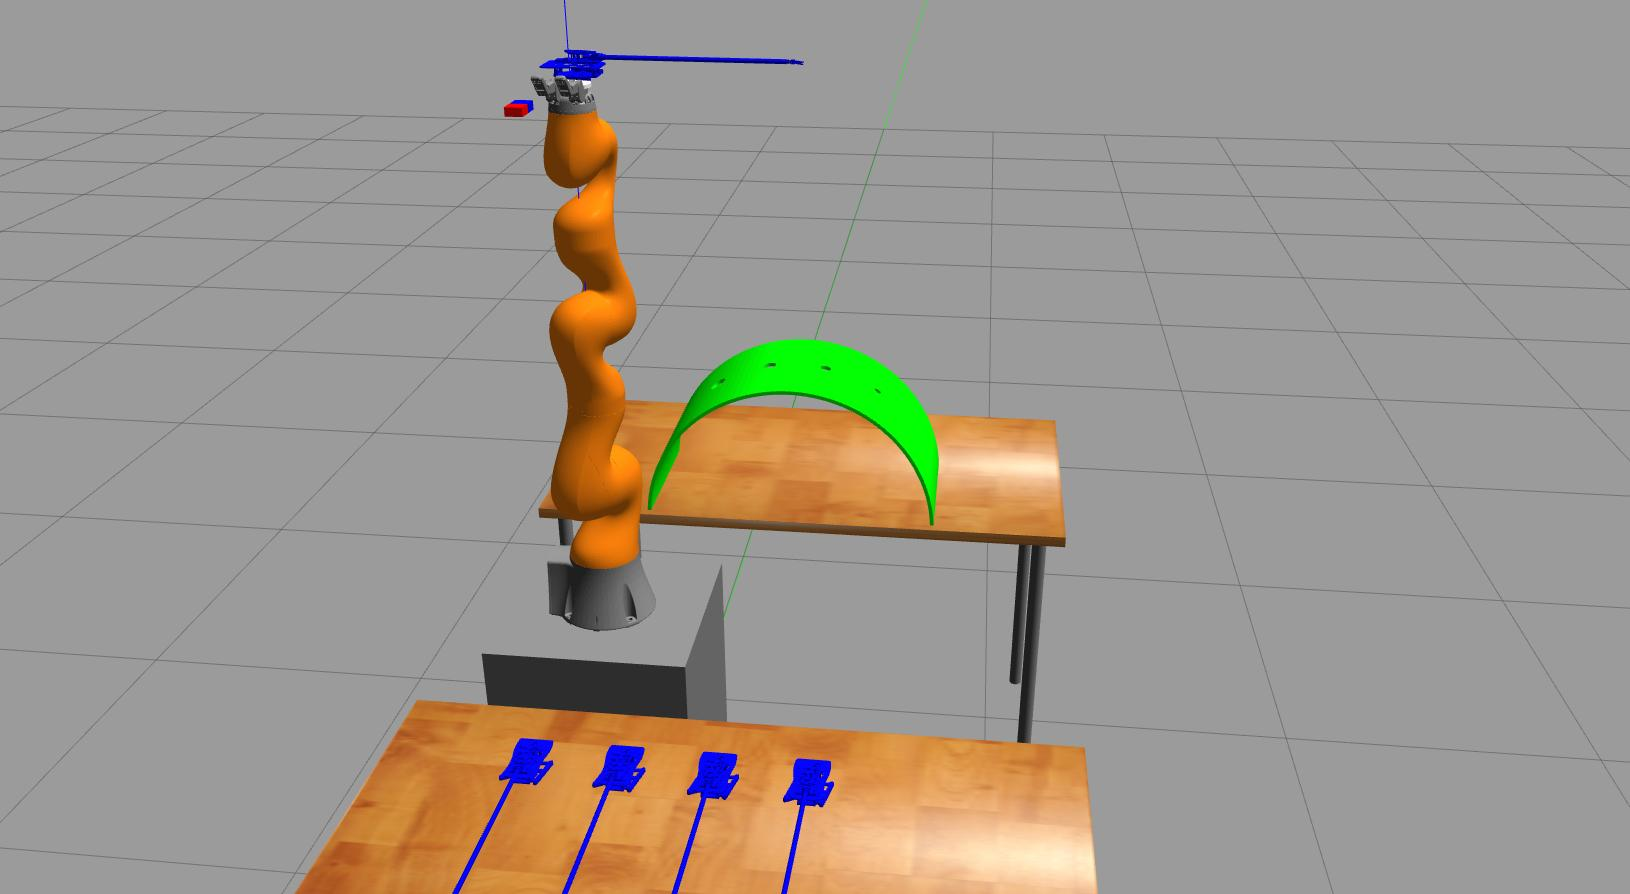
\includegraphics[width=0.31\textwidth]{images/robot_planner2/robot_planner2_1}
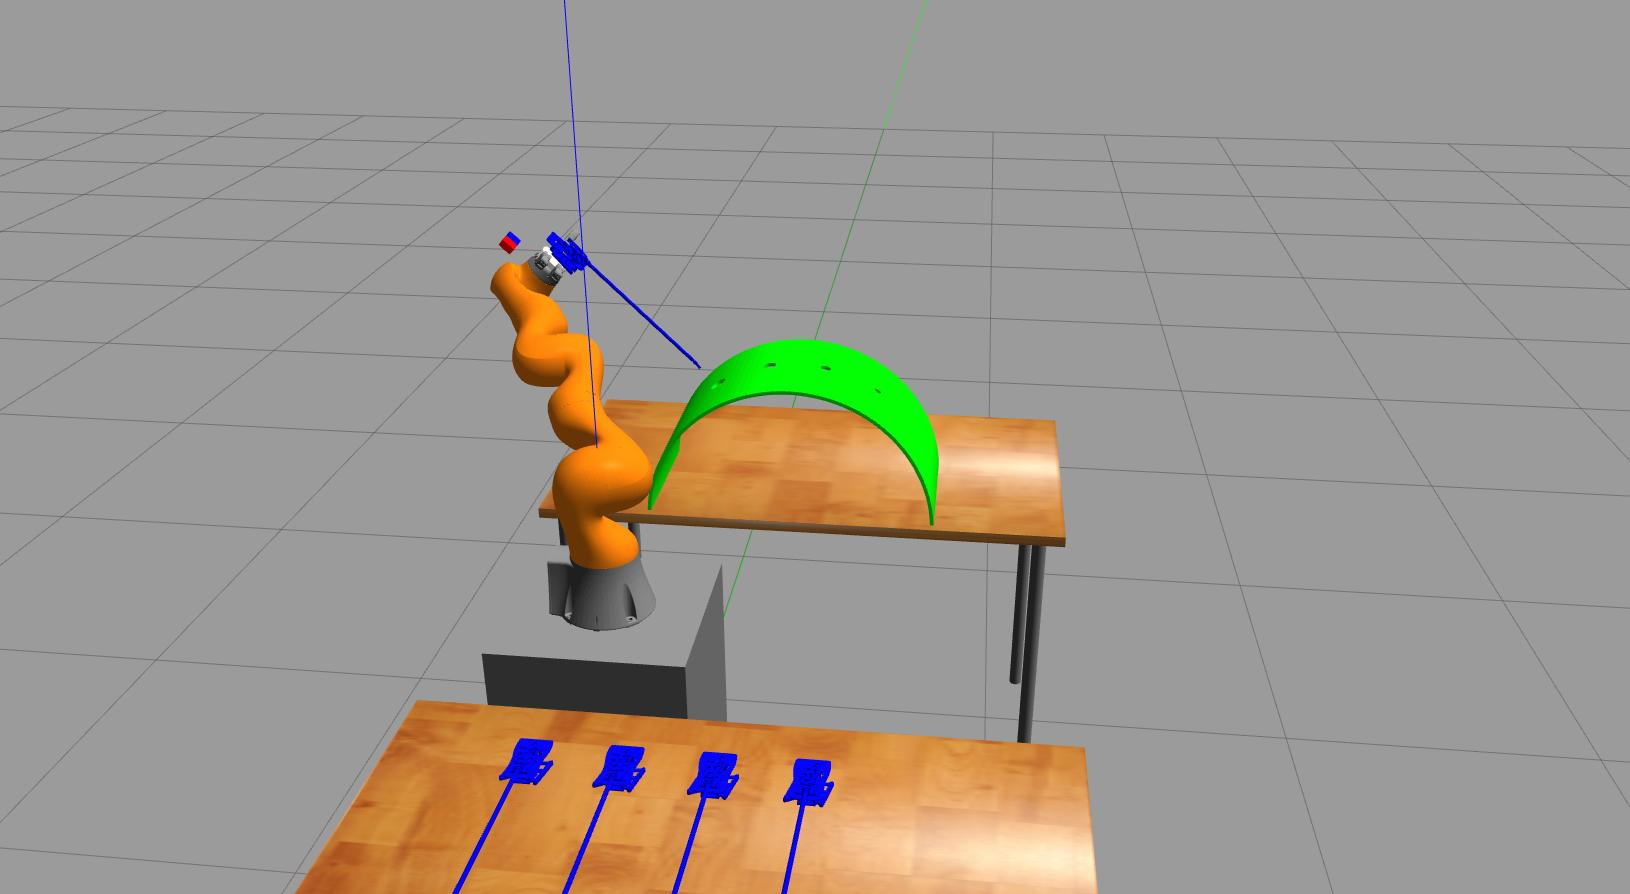
\includegraphics[width=0.31\textwidth]{images/robot_planner2/robot_planner2_2}
\includegraphics[width=0.31\textwidth]{images/robot_planner2/robot_planner2_3}\\
\includegraphics[width=0.31\textwidth]{images/robot_planner2/robot_planner2_4}
\includegraphics[width=0.31\textwidth]{images/robot_planner2/robot_planner2_5}
\includegraphics[width=0.31\textwidth]{images/robot_planner2/robot_planner2_6}\\
\includegraphics[width=0.31\textwidth]{images/robot_planner2/robot_planner2_7}
\includegraphics[width=0.31\textwidth]{images/robot_planner2/robot_planner2_8}\\
\caption{Experiment 2a:}
\label{experiment-robot-planner2a}
\end{figure}
\end{center}

% Robot Planner 2a with RRTConnect
\begin{longtable}{|p{2cm}|c|p{2cm}|p{2cm}|p{2cm}|}
\hline
Robot Planner 2a           & \multicolumn{4}{c}{\textbf{RRTConnect}}                                                                                                 \vline \\
\hline
                          & \multicolumn{4}{c}{\textbf{Insertion \& Pivot trajectories}}                     \vline \\
\hline
Experiment                & Trocar1 insertion time & Execution status & Trocar1 retraction time & Execution status  \\
\hline
1	& 0.060728	& 1	& 2.875072	& 1 \\
2	& 0.070508	& 1	& 5.235667	& 1 \\
3	& 0.071487	& 1	& 5.239014	& 1 \\
4	& 0.059288	& 1	& 1.733352	& 1 \\
5	& 0.053619	& 1	& 3.376982	& 1 \\
6	& 0.062	& 1	& 5.389454	& 1 \\
7	& 0.084007	& 1	& -	& 0 \\
8	& 0.058306	& 1	& 5.254352	& 1 \\
9	& 0.046925	& 1	& 4.90185	& 1 \\
10	& 0.060491	& 1	& 5.073171	& 1 \\
\hline
\textbf{Average} & 	0.062736	& 1	& 4.342102	& 0.9 \\
\hline
                          & \multicolumn{4}{c}{\textbf{Insertion \& Pivot trajectories}}                     \vline \\
\hline
Experiment                & Approach trocar2 time & Execution status & Trocar2 insertion time & Execution status  \\
\hline
1 & 2.67618	& 1	& 0.168283	& 1 \\
2 & 5.187283	& 1	& 0.179048	& 1 \\
3 & 0.050117	& 1	& 0.057194	& 1 \\
4 & 1.538822	& 1	& 0.184641	& 1 \\
5 & 1.62114	& 1	& 0.253224	& 1 \\
6 & 5.397757	& 1	& 0.268188	& 1 \\
7 & 5.379305	& 1	& 0.384924	& 1 \\
8 & 5.401832	& 1	& 0.193265	& 1 \\
9 & 2.845741	& 1	& 0.267069	& 1 \\
10  & 5.355111	& 1	& 0.250265	& 1 \\
\hline
\textbf{Average} & 3.545329	& 1	& 0.220610	& 1 \\
\hline
                          & \multicolumn{4}{c}{\textbf{Insertion \& Pivot trajectories}}                     \vline \\
\hline
Experiment                & Trocar2 retraction time & Execution status & Approach trocar3 time & Execution status  \\
\hline
1 & 0.152233	& 1	& 0.214332	& 1 \\
2 & 0.321677	& 1	& 0.361712	& 1 \\
3 & 5.404121	& 1	& 5.271597	& 1 \\
4 & 0.147981	& 1	& 0.15915	& 1 \\
5 & 0.333447	& 1	& 0.298799	& 1 \\
6 & 0.246624	& 1	& 0.209347	& 1 \\
7 & 0.381983	& 1	& 0.473779	& 1 \\
8 & 0.219369	& 1	& 0.167211	& 1 \\
9 & 0.227563	& 1	& 0.297372	& 1 \\
10  & 5.149372	& 1	& 5.3578	& 1 \\
\hline
\textbf{Average} & 1.258437	& 1	& 1.281110	& 1 \\
\hline
                          & \multicolumn{4}{c}{\textbf{Insertion \& Pivot trajectories}}                     \vline \\
\hline
Experiment                & Trocar3 insertion time & Execution status & Trocar3 retraction time & Execution status  \\
\hline
1 & 0.196175	& 1	& 0.855452	& 0 \\
2 & 0.412455	& 1	& 1.133213	& 0 \\
3 & 0.355923	& 1	& 0.814161	& 0 \\
4 & 0.194839	& 1	& 0.885119	& 0 \\
5 & 0.351561	& 1	& 0.364089	& 0 \\
6 & 0.355251	& 1	& 0.826636	& 0 \\
7 & 0.336123	& 1	& 0.30715	& 1 \\
8 & 0.147867	& 1	& 1.053035	& 0 \\
9 & 0.347956	& 0.6	& 0.80884	& 0.37  \\
10  & 0.28364	& 0.6	& 0.229825	& 1 \\
\hline
\textbf{Average} & 	0.298179	& 0.92 &	0.727752	& 0.237 \\
\hline

\caption{Time results for robot planner 2a using the RRTConnect path planner algorithm. Planning time is the sum of solution time and path simplification time. Execution status is 
1 for success and 0 for failure. Parameters: tolerances: 0.0005, max planning time: 5 seconds, replanning: true, max planning attempts: 6. Experiments start from home position.}
\label{robot-planner2a-rrtconnect-data}
\end{longtable}

To overcome the reachability issue shown in Figure \ref{experiment-robot-planner2a}, the algorithm was repeated, but this time using a different simulation layout 
in Gazebo, in which the mounting dock is closer to the robot and in front of it. This new layout enables the robot to reach all mounting holes with ease and 
with sufficient dexterity, the robot is free to pivot around.

\begin{center}
\begin{figure}[!htb]
\centering
\includegraphics[width=0.3\textwidth]{images/robot_planner2b/robot_planner2b_1}
\includegraphics[width=0.3\textwidth]{images/robot_planner2b/robot_planner2b_2}
\includegraphics[width=0.3\textwidth]{images/robot_planner2b/robot_planner2b_3}\\
\includegraphics[width=0.3\textwidth]{images/robot_planner2b/robot_planner2b_4}
\includegraphics[width=0.3\textwidth]{images/robot_planner2b/robot_planner2b_5}
\includegraphics[width=0.3\textwidth]{images/robot_planner2b/robot_planner2b_6}\\
\includegraphics[width=0.3\textwidth]{images/robot_planner2b/robot_planner2b_7}
\includegraphics[width=0.3\textwidth]{images/robot_planner2b/robot_planner2b_8}
\includegraphics[width=0.3\textwidth]{images/robot_planner2b/robot_planner2b_9}\\
\caption{Experiment 2b: Running robot planner 2b with a different table layout so that all target poses have improved reachability. Note that all trajectories shown in the screenshots are collision-free, 
because the robotic arm is in an elbow-up configuration, so that it avoids the collision between the 3rd link of the robot and the mounting dock (green object shown in simulation).}
\label{experiment-robot-planner2b}
\end{figure}
\end{center}

Observing the screenshots at figure \ref{experiment-robot-planner2b}, it is clear that the robot must always be in an elbow-up configuration in order to avoid collisions with the mounting dock. This constraint can be 
described either using the relative distance of the third link with the base or the relative angles of the third link's axis with respect to the axis of the base, as described with more detail in 
\ref{section-elbow-up-constraints}. The latter description with angles is easier to implement using the ROS MoveIt! framework,  but it would require to solve an extra inverse and forward kinematics problem targeting the third 
link, instead of the end-effector. To avoid these additional, computationally expensive calculations and simplify the experiments, instead of mathematically describing the constraint, 
some extra points were added in the trajectory. 
These points are usually close to the robot's axis and are such, that 
moveit will be forced to find a solution with an elbow-up configuration (because there will be no other solution satisfying the target point). Starting with an elbow-up configuration makes the path planner stick with that 
configuration for most of the path, because otherwise it would make a big jump in the joint state space which is not allowed from the parameters used in the experiments.

% Robot Planner 2b with RRTConnect
\begin{longtable}{|p{2cm}|c|p{2cm}|p{2cm}|p{2cm}|}
\hline
Robot Planner 2b           & \multicolumn{4}{c}{\textbf{RRTConnect}}                                                                                                 \vline \\
\hline
                          & \multicolumn{4}{c}{\textbf{Insertion \& Pivot trajectories}}                     \vline \\
\hline
Experiment                & Trocar1 insertion time & Execution status & Trocar1 retraction time & Execution status  \\
\hline
1	& 0.269901	& 1	& 0.355588	& 1 \\
2	& 0.220509	& 1	& 0.255968	& 1 \\
3	& 0.260483	& 1	& 5.28604	& 1 \\
4	& 0.267778	& 1	& 0.267796	& 1 \\
5	& 0.388487	& 1	& 5.321684	& 1 \\
6	& 0.316275	& 1	& 0.2088	& 1 \\
7	& 0.202614	& 1	& 0.14469	& 1 \\
8	& 0.289368	& 1	& 0.275917	& 1 \\
9	& 0.353631	& 1	& 0.353631	& 1 \\
10	& 0.185345	& 1	& 0.154755	& 1 \\
\hline
\textbf{Average} & 0.275439 &	1	& 1.262487	& 1 \\
\hline
                          & \multicolumn{4}{c}{\textbf{Insertion \& Pivot trajectories}}                     \vline \\
\hline
Experiment                & Approach trocar2 time & Execution status & Trocar2 insertion time & Execution status  \\
\hline
1 & 0.322578	& 1	& 0.283497	& 1 \\
2 & 0.209871	& 1	& 0.410543	& 1 \\
3 & 5.099769	& 1	& 0.296228	& 1 \\
4 & 0.216997	& 1	& 0.342776	& 1 \\
5 & 5.328204	& 1	& 0.394472	& 1 \\
6 & 0.450936	& 1	& 0.249248	& 1 \\
7 & 0.336209	& 1	& 0.165375	& 1 \\
8 & 0.397699	& 1	& 0.202118	& 1 \\
9 & 0.235555	& 1	& 0.333129	& 1 \\
10  & 0.320059	& 1	& 0.343595	& 1 \\
\hline
\textbf{Average} & 1.291788	& 1	& 0.302098	& 1 \\
\hline
                          & \multicolumn{4}{c}{\textbf{Insertion \& Pivot trajectories}}                     \vline \\
\hline
Experiment                & Trocar2 retraction time & Execution status & Approach trocar3 time & Execution status  \\
\hline
1 & 5.374646	& 1	& 5.451335	& 1 \\
2 & 0.452231	& 1	& 0.253669	& 1 \\
3 & 0.22638	& 1	& 0.383933	& 1 \\
4 & 5.371822	& 1	& 5.611649	& 1 \\
5 & 0.395787	& 1	& 0.309212	& 1 \\
6 & 5.15406	& 1	& 5.515007	& 1 \\
7 & 4.189377	& 1	& 5.570568	& 1 \\
8 & 5.167346	& 1	& 5.522056	& 1 \\
9 & 5.101735	& 1	& 5.452301	& 1 \\
10  & 5.273342	& 1	& 5.467273	& 1 \\
\hline
\textbf{Average} & 3.670673	& 1	& 3.953700	& 1 \\
\hline
                          & \multicolumn{4}{c}{\textbf{Insertion \& Pivot trajectories}}                     \vline \\
\hline
Experiment                & Trocar3 insertion time & Execution status & Trocar3 retraction time & Execution status  \\
\hline
1 & 0.372382	& 1	& 5.34059	& 1 \\
2 & 0.280432	& 1	& 0.261765	& 1 \\
3 & 0.179581	& 1	& 0.187589	& 1 \\
4 & 0.121094	& 1	& 5.152808	& 1 \\
5 & 0.472468	& 1	& -	& 0 \\
6 & 0.251195	& 1	& 0.442282	& 0 \\
7 & 0.20647	& 1	& 0.318481	& 1 \\
8 & 0.178941	& 1	& 0.185758	& 1 \\
9 & 0.188906	& 1	& 0.222821	& 1 \\
10  & 0.165681	& 1	& 0.170876	& 1 \\
\hline
\textbf{Average} & 	0.241715  &	1 &	1.364774 &	0.8 \\
\hline
\caption{Time results for robot planner 2b using the RRTConnect path planner algorithm and a different table layout from robot planner 2a. Planning time is the sum of solution time and path simplification time. Execution status is 
1 for success and 0 for failure. Parameters: tolerances: 0.0005, max planning time: 5 seconds, replanning: true, max planning attempts: 6. Experiments start from home position.}
\label{robot-planner2b-rrtconnect-data}
\end{longtable}


Due to the probabilistic nature of the motion planner (in these experiments the OMPL library is used with the RRTConnect path planning algorithm), the solutions 
to the path planning problem are not always the same and thus it is possible that the robot arm reaches a pose which is close to a singularity
\begin{center}
\begin{figure}[!htb]
\centering
\includegraphics[width=0.9\textwidth]{images/robot_planner2b/singularity_failure.png}
\caption{Experiment 2b: Singularity failure}
\label{robot-planner2b-singularity-failure}
\end{figure}
\end{center}

Sometimes, when planning or executing a trajectory the robot may fail to complete the task because it has approached a singularity point. The points of singularity or of low dexterity are those points shown in the screenshot 
\ref{robot-planner2b-singularity-failure} which have red color. The color coding is calculated using the equation \ref{dexterity-measure}. The values of the Jacobian matrix are calculated at every kinematic state using 
a custom ROS node that subscribes to the robot's kinematic state (joints' angle positions, velocities, etc) and publishes the values of the Jacobian matrix as well as the forward kinematics solutions, to the 
/kinematic\_state topic (see figure \ref{kinematic-state-topic-graph}).

\begin{center}
\begin{figure}[!htb]
\centering
\includegraphics[width=\textwidth]{images/kinematic_state_topic_graph.png}
\caption{Custom kinematic state node that subscribes to the joint values and publishes forward kinematics solutions and the jacobian matrix values.}
\label{kinematic-state-topic-graph}
\end{figure}
\end{center}


\section{Robot Planner 3: Trajectory planning}

The goal of this third experiment is to design and test only some pivot trajectories. The pivot motions follow the equations described in 
\ref{section:pivot-motions}. The trajectories that were designed and tested in this group of experiments are the following:
\begin{itemize}
\item Line segment
\item Circle
\item Cubic spline
\item B-Spline
\item Quintic polynomial in joint space
\item Trapezoidal velocity profile in joint space
\item S-Curve velocity profile in joint space
\item Helix
\end{itemize}

\subsection{Line segment trajectories in task space}

The goal of this experiment is to generate a line segment trajectory inside the surgical
taskspace which will then be transformed via the fulcrum transformation to a trajectory that the robotic arm can execute. To define a line segment only 
2 points are needed, the coordinates of the start and those of the end of the line segment. An other, way of defining a line segment trajectory, 
is by passing as parameters the coordinates of the start point and a vector attached to that point, whose and points to the end point. The second definition 
of the line segment can be very useful in cases where the direction of the line is needed.

\begin{center}
\begin{figure}[!htb]
\centering
\includegraphics[width=\textwidth]{images/robot_planner3/3b_line_seg.png}
\caption{Experiment 3b: Create the line segment trajectory inside the surgical site (below the green mounting dock) and transform it via the fulcrum transformation to a trajectory for the robot's TCP.
(a) Preparatory path to achieve elbow-up pose, (b) transformed line segment trajectory for the end-effector to follow, (c) transformed line segment trajectory with respect to the tool base frame (there is an offset from the 
end-effector see \ref{section:eef-tool-tip-transformations}), (d) fulcrum reference frame 2 $\lbrace F_2 \rbrace$, (e) line segment trajectory in surgical taskspace, (f) line of the axis along the length of the surgical tool, 
which is used to calculated the distance error (RCM deviation)}
\label{robot-planner3b-line-seg}
\end{figure}
\end{center}

\begin{center}
\begin{figure}[!htb]
\centering
\includegraphics[width=0.49\textwidth]{images/robot_planner3/robot_planner3b_error1.png}
\includegraphics[width=0.49\textwidth]{images/robot_planner3/robot_planner3b_error2.png}
\caption{Experiment 3b: RCM errors from two iterations of the same experiment. The robot starts from the home position where the rcm error is bigger, then approaches the fulcrum point, where the errors decreases and then 
it executes the line segment pivot trajectory where the error is bounded in the magnitude of less than a micrometer $10^{-6}m$. The x-axis shows the ROS time in seconds and the y-axis the RCM error in logarithmic scale.}
\label{robot-planner3b-line-seg-rcm-errors}
\end{figure}
\end{center}

Note that although this type of trajectory is trivial in robot planner, this specific line segment trajectory should not be confused with ROS MoveIt line segment trajectories. The line-segment studied in this experiment 
is linear when defined in the surgical taskpsace, but it is highly non-linear when transformed via the fulcrum transformation and it has a curved shape. The only exceptions to this transformation is for line segments that 
lie on the direction defined by the radius unit vector $\mathbf{\hat{r}}$ of the spherical coordinate system of the Fulcrum reference frame, or equivalently the points $A,B$ defining the line-segment and the origin $O$ 
of the reference frame, must be collinear. These exceptions can also be planned by the MoveIt framework and are also known 
as and referenced throughout this thesis, as insertion movements. Let $\overrightarrow{AB}$ be the vector representing the line segment, then for the points $A, B$ the following must hold, in order for the line segment to be 
invariant under the fulcrum transformation in terms of shape (i.e. the line to remain a line).
\begin{equation}
\overrightarrow{AB} = \overrightarrow{OB} - \overrightarrow{OA}
\end{equation} 
and
\begin{equation}
\overrightarrow{OB} = r \overrightarrow{OA}, \quad r \in \mathbb{R}
\end{equation}

\begin{center}
\begin{figure}[!htb]
\centering
\includegraphics[width=\textwidth]{images/robot_planner3/3b_line_seg_invariant.png}
\caption{Experiment 3b: Line segment trajectory that is invariant under the fulcrum transformation, in terms of shape (the line remains a line).}
\label{robot-planner3b-line-seg}
\end{figure}
\end{center}


\subsection{Circular trajectories in task space}

The goal of this experiment is to generate a circular trajectory inside the surgical taskspace which will then be transformed via the fulcrum transformation 
to a trajectory that the robotic arm can execute. To define a circular trajectory in the taskspace, two parameters are required: the $(x,y,z)$ coordinates of the 
circle's center and it's radius $r$.\\ 

\begin{center}
\begin{figure}[!htb]
\centering
\includegraphics[width=\textwidth]{images/robot_planner3/3a_circle.png}
\caption{Experiment 3a: Create circular trajectory inside the surgical site (below the green mounting dock) and transform it via the fulcrum transformation to a trajectory for the robot's TCP.}
\label{robot-planner3a-circle}
\end{figure}
\end{center}

\begin{center}
\begin{figure}[!htb]
\centering
\includegraphics[width=\textwidth]{images/robot_planner3/3a_circle_details.png}
\caption{Experiment 3a: }
\label{robot-planner3a-circle-details}
\end{figure}
\end{center}

Note that in this experiment (see screenshot \ref{robot-planner3a-circle}), the trivial case is examined where the circle is parallel to the $xy$ plane of the fulcrum's 
coordinate system. That is because the parametric definition if the circle, can be easily expressed when in a standard plane of the coordinate system i.e. $xy, xz$ 
or $yz$ planes and not in an arbitrary orientation.

% Robot Planner 3a with RRTConnect
% \begin{table}[H]
% \centering
% \begin{tabular}{|p{2cm}|c|p{3cm}|p{3cm}|p{3cm}|}
% \hline
% Robot Planner 3a           & \multicolumn{4}{c}{\textbf{RRTConnect}}                                                                                                 \vline \\
% \hline
%                           & \multicolumn{4}{c}{\textbf{Place \& Insert tool}}                     \vline \\
% \hline
% Experiment                & Status & Solution Time & Path Simplification Time & Planning Attempts  \\
% \hline
% 1                         &        &               &                          &  \\
% 2                         &        &               &                          &  \\
% 3                         &        &               &                          &  \\
% 4                         &        &               &                          &  \\
% 5                         &        &               &                          &  \\
% \hline
% \textbf{Average} & 	& 	& 	&  \\
% \hline
%                           & \multicolumn{4}{c}{\textbf{Pivot Trajectory}}                     \vline \\
% \hline
% Experiment                & Status & Solution Time & Path Simplification Time & Planning Attempts  \\
% \hline
% 1                         &        &               &                          &  \\
% 2                         &        &               &                          &  \\
% 3                         &        &               &                          &  \\
% 4                         &        &               &                          &  \\
% 5                         &        &               &                          &  \\
% \hline
% \textbf{Average} & 	& 	& 	&  \\
% \hline
% \end{tabular}
% \caption{Time results for robot planner 3a using the RRTConnect path planner algorithm}
% \label{robot-planner3a-rrtconnect-data}
% \end{table}


\subsection{Cubic Spline trajectories in task space}

The goal of this experiment is to generate a cubic spline trajectory inside the surgical
taskspace which will then be transformed via the fulcrum transformation to a trajectory that the robotic arm can execute.

\begin{center}
\begin{figure}[!htb]
\centering
\includegraphics[width=\textwidth]{images/robot_planner3/3c_cubic_spline.png}
\caption{Experiment 3c: Create the cubic spline trajectory inside the surgical site (below the green mounting dock) and transform it via the fulcrum transformation to a trajectory for the robot's TCP.}
\label{robot-planner3c-cubic-spline}
\end{figure}
\end{center}

As seen on the screenshot \ref{robot-planner3c-cubic-spline}, for the surgical task there are 4 four points that were selected to create 3 cubic splines. The points that define the trajectory were:
\[
\begin{aligned}
\mathbf{x}_1 ={}& [-0.1, -0.1, -0.2] \\
\mathbf{x}_2 ={}& [0.1, -0.1, -0.1] \\
\mathbf{x}_3 ={}& [0.1, 0.1, -0.2] \\
\mathbf{x}_4 ={}& [-0.1, -0.1, -0.2] = \mathbf{x}_1
\end{aligned}
\]

and a constant derivative for all points of $\mathbf{x}_d = [0.1, 0.1, 0.1]$. Note that this derivative describes the shape and smoothness at the points that connect 
2 consecutive splines. These derivatives may not necessarily express a velocity in the cartesian space. That is because this derivative is calculated with respect 
to the path variable $s$. The time derivative of the trajectory would be calculated using the chain rule:

\begin{equation}
\begin{aligned}
\mathbf{\dot{x}} ={}& \frac{d\mathbf{x}}{dt}  \\
	={}& \frac{d\mathbf{x}(s)}{dt} = \frac{d\mathbf{x}(s(t))}{dt}   \\
    ={}& \frac{d\mathbf{x}}{ds} \cdot \frac{ds}{dt} \\
    ={}& \mathbf{x}_d \cdot \frac{ds}{dt}
\end{aligned}
\end{equation}


\subsection{B-Spline trajectories in task space}

\begin{center}
\begin{figure}[!htb]
\centering
\includegraphics[width=\textwidth]{images/robot_planner3/3d_bezier_spline.png}
\caption{Experiment 3d: Create the B-spline trajectory inside the surgical site (below the green mounting dock) and transform it via the fulcrum transformation to a trajectory for the robot's TCP.}
\label{robot-planner3d-bezier-spline}
\end{figure}
\end{center}


\subsection{Polynomial trajectories in joint space}
\label{section:9-2-polynomial-traj}

The goal of this experiment is to generate a trajectory in joint space using a polynomial of 5th degree (see \ref{section-polynomials-5}). To generate this trajectory, at least 2 points are needed in the cartesian 
space. For each of these points the inverse kinematics problem is solved. The joint values of the first point are used as the start points of the trajectory and the joint values of the second point are used as the end points.
The velocities and accelerations are chosen to be zero for both start and end positions. The poses of the 2 points that were used as input to the 2 IK problems are

\[
T_A = 
\begin{bmatrix}
  &            &   & 0.1 \\
  & \mathbf{R_{rpy}} &   & 0.1 \\
  &            &   & 1.95 \\
0 &     0      & 0 & 1 \\
\end{bmatrix}
\]
\[
T_B = 
\begin{bmatrix}
  &            &   & 0.4 \\
  & \mathbf{R_{rpy}} &   & 0.1 \\
  &            &   & 1.95 \\
0 &     0      & 0 & 1 \\
\end{bmatrix}
\]
where 
\[
\mathbf{R_{rpy}} = \mathbf{Rot}(\mathbf{\hat{z}}, 2.952052) \cdot \mathbf{Rot}(\mathbf{\hat{y}}, 1.311528) \cdot \mathbf{Rot}(\mathbf{\hat{x}}, -1.750799)
\]

and the solutions chosen for each point are

\[
\mathbf{q_A} =
\begin{bmatrix}
1.148534 \\
-0.583084 \\ 
-0.212395 \\ 
-1.430756 \\
0.609015 \\ 
1.168518 \\ 
-0.523555 \\
\end{bmatrix}
\quad \textrm{and} \quad
\mathbf{q_B} = 
\begin{bmatrix}
2.293053 \\ 
-0.277892 \\
-1.795364 \\ 
-0.941923 \\ 
0.876039 \\
1.451593 \\
-0.916277 \\
\end{bmatrix}
\]

\begin{center}
\begin{figure}[H]
\centering
\includegraphics[width=\textwidth]{images/robot_planner3/3e_joint_polynomial.png}
\caption{Experiment 3e: Polynomial trajectories of 5th degree for each of the 7 joints. The trajectory is computed at 60 sampling points.}
\label{robot-planner3e-joint-polynomial}
\end{figure}
\end{center}


\subsection{Trajectories in joint space with trapezoidal velocity profile}

The goal of this experiment is to generate a trajectory in joint space using a trapezoidal velocity profile. The start and end points as well as the inverse kinematics solutions for these points are the same as those 
in \ref{section:9-2-polynomial-traj}.

\begin{center}
\begin{figure}[H]
\centering
\includegraphics[width=\textwidth]{images/robot_planner3/3f_trapezoid1.png}
\caption{Experiment 3f: Trajectory using a trapezoid velocity profile. The time constant (also known as blend time) is $τ = 15$ seconds and the total trajectory duration is 60 seconds. The trajectory is computed at 60 sampling points.}
\label{robot-planner3f-joint-trapezoid1}
\end{figure}
\end{center}

\begin{center}
\begin{figure}[H]
\centering
\includegraphics[width=\textwidth]{images/robot_planner3/3f_trapezoid2.png}
\caption{Experiment 3f: Trajectory using a trapezoid velocity profile. The time constant (also known as blend time) is $τ = 30$ seconds and the total trajectory duration is 60 seconds. Note that 
the blend time is chosen as half of the total duration which has as a result the linear segment (constant velocity) to disappear and create a "bang-bang" trajectory. In control theory, a "bang-bang" controller, 
is a controller that switches abruptly between two states. The trajectory is computed at 60 sampling points.}
\label{robot-planner3f-joint-trapezoid2}
\end{figure}
\end{center}


\subsection{Trajectories in joint space with s-curve velocity profile}

The goal of this experiment is to generate a trajectory in joint space using a smooth s-curve velocity profile. The start and end points as well as the inverse kinematics solutions for these points are the same as those 
in \ref{section:9-2-polynomial-traj}.

\begin{center}
\begin{figure}[H]
\centering
\includegraphics[width=\textwidth]{images/robot_planner3/3g_s_curve.png}
\caption{Experiment 3g: Trajectory using a s-curve velocity profile. The time constants are $τ_1 = τ_2 = 6$ seconds and the total trajectory duration is 60 seconds. The trajectory is computed at 60 sampling points.}
\label{robot-planner3g-joint-s-curve}
\end{figure}
\end{center}


\subsection{Helical trajectories in task space}

The goal of this experiment is to generate a helical trajectory inside the surgical taskspace which will then be transformed via the fulcrum transformation 
to a trajectory that the robotic arm can execute. To define a helical trajectory in the taskspace, two parameters are required: the $(x,y,z)$ coordinates of the 
helix center, it's radius $r$, as well as the number of cycles $τ$ of the helix and slope parameter $β$.\\ 

\begin{center}
\begin{figure}[!htb]
\centering
\includegraphics[width=\textwidth]{images/robot_planner3/3h_helix.png}
\caption{Experiment 3h: Create helical trajectory inside the surgical site (below the green mounting dock) and transform it via the fulcrum transformation to a trajectory for the robot's TCP.}
\label{robot-planner3h-helix}
\end{figure}
\end{center}


\section{Robot Planner 4: Simple cube pick-and-place experiment}

In this experiment we plan a simple pick-and-place path for a cube. The robotic arm first visits the left table and starts from the pre-grasp posture and then 
slowly approaches the cube until the grasp posture. When the gripper has reached the grasp posture, it closes the fingers to grasp the object and then retreats 
to the post-grasp posture. After that the robotic arm visits the right table to execute the place steps which are similar to the pick steps. The images below 
show some frames from the experiment with the first three to show the pick steps in the simulation environment and then other three images show the place steps 
in the visualization program.

\begin{center}
\begin{figure}[!htb]
\centering
\includegraphics[width=0.3\textwidth]{images/robot_planner4/robot_planner4_1}
\includegraphics[width=0.3\textwidth]{images/robot_planner4/robot_planner4_3}
\includegraphics[width=0.3\textwidth]{images/robot_planner4/robot_planner4_5}\\
\includegraphics[width=0.3\textwidth]{images/robot_planner4/robot_planner4_6}
\includegraphics[width=0.3\textwidth]{images/robot_planner4/robot_planner4_8}
\includegraphics[width=0.3\textwidth]{images/robot_planner4/robot_planner4_10}\\
\caption{Experiment 4: Simple pick-and-place experiment of a cube}
\end{figure}
\end{center}

Observing the results from table \ref{robot-planner4-rrtconnect-data}, the time duration for the pick pipeline of this experiment using the RRTConnect path planning algorithm, 
ranges from approximately 0.01 to 0.02 seconds, whereas in the Place pipeline we observe mainly 2 distinct groups of time ranges. One group has values around 0.02 seconds and the other 
has bigger values around 0.14 seconds. In the case with the bigger time durations, the solution made the robot go around the obstacle whereas in the other cases the path planning solution avoided the obstacle, 
which means that an easier path was found, it was solved quicker and the path solution was much simpler (in terms of kinematic constraints) which led to smaller path simplification time durations. 
It is also possible, that due to the obstacle and the initial conditions, the robot may not find a solution at the first attempt or none at all.

% Robot Planner 4 with RRTConnect
\begin{longtable}{|p{2cm}|c|p{3cm}|p{3cm}|p{3cm}|}
\hline
Robot Planner 4           & \multicolumn{4}{c}{\textbf{RRTConnect}}                                                                                                 \vline \\
\hline
                          & \multicolumn{4}{c}{\textbf{Pick Pipeline}}                     \vline \\
\hline
Experiment                & Status & Solution Time & Path Simplification Time & Planning Attempts  \\
\hline
1 & 1 & 0.026189 & 0.065173 & 1 \\
2 & 1 & 0.016835 & 0.043333 & 1 \\
3 & 1 & 0.025439 & 0.023178 & 1 \\
4 & 1 & 0.029292 & 0.066913 & 1 \\
5 & 1 & 0.024873 & 0.01747 & 1 \\
6 & 1 & 0.017615 & 0.024568 & 1 \\
7 & 1 & 0.014263 & 0.028095 & 1 \\
8 & 1 & 0.015479 & 0.027035 & 1 \\
9 & 1 & 0.027803 & 0.057064 & 1 \\
10 & 1 & 0.026057 & 0.033179 & 1 \\
\hline
\textbf{Average} & 1	& 0.02196178	& 0.0386008	& 1 \\
\hline
                          & \multicolumn{4}{c}{\textbf{Place Pipeline}}                     \vline \\
\hline
Experiment                & Status & Solution Time & Path Simplification Time & Planning Attempts  \\
\hline
1 & 1 & 0.014644 & 0.020947 & 1 \\
2 & 1 & 0.131334 & 0.938948 & 1 \\
3 & 1 & 0.021425 & 0.08429 & 1 \\
4 & 1 & 0.01675 & 0.01675 & 1 \\
5 & 1 & 0.165795 & 1.661019 & 1 \\
6 & 1 & 0.119819 & 0.394493 & 1 \\
7 & 1 & 0.140645 & 0.476835 & 1 \\
8 & 1 & 0.133917 & 0.673233 & 1 \\
9 & 1 & 0.017644 & 0.038319 & 1 \\
10 & 1 & 0.020025 & 0.074847 & 1 \\
\hline
\textbf{Average} & 1	& 0.0781998	& 0.4379681	& 1 \\
\hline
\caption{Time results for robot planner 4 using the RRTConnect path planner algorithm}
\label{robot-planner4-rrtconnect-data}
\end{longtable}

The main observation from the results of table \ref{robot-planner4-rrtstar-data} is that RRT* time durations are much bigger than those from RRTConnect, but the RRT* algorithm has the advantage of finding better, more accurate solutions (approximately the same solutions at most attempts) and with less collisions. Although these time durations are not optimal for real-time applications, they could be useful in pick-and-place pipelines 
if the solutions are pre-computed (memoized) and saved for later use.

% Robot Planner 4 with RRT*
\begin{longtable}{|p{2cm}|c|p{3cm}|p{3cm}|p{3cm}|}
\hline
Robot Planner 4           & \multicolumn{4}{c}{\textbf{RRT*}}                                                                                                 \vline \\
\hline
                          & \multicolumn{4}{c}{\textbf{Pick Pipeline}}                     \vline \\
\hline
Experiment                & Status & Solution Time & Path Simplification Time & Planning Attempts  \\
\hline
1	& 1 & 44.97476	& 0.030918	& 1	\\
2	& 1 & 45.006897	& 0.073009	& 1	\\
3	& 1	& 44.989085	& 0.053440	& 1	\\
4	& 1 & 44.998414	& 0.034571	& 1	\\
5	& 1 & 44.982524	& 0.041732	& 1	\\
6	& 1 & 44.997148	& 0.017660	& 1	\\
7	& 1 & 45.00115	& 0.022290	& 1	\\
8	& 1 & 44.991409	& 0.046728	& 1	\\
\hline
\textbf{Average} & 1 & 44.99267	& 0.0400435	& 1	\\
\hline
                          & \multicolumn{4}{c}{\textbf{Place Pipeline}}                     \vline \\
\hline
Experiment                & Status & Solution Time & Path Simplification Time & Planning Attempts  \\
\hline
1	& 1	& 45.064568	& 0.884821	& 1 \\
2	& 1	& 44.965931	& 0.054692	& 1 \\
3	& 1	& 44.976697	& 0.012784	& 1 \\
4	& 1	& 44.968431	& 0.020354	& 1 \\
5	& 1	& 45.068239	& 0.551800	& 1 \\
6	& 1	& 45.016043	& 1.089529	& 1 \\
7	& 1	& 45.048851	& 0.680121	& 1 \\
8	& 1	& 45.023364	& 0.000004	& 1 \\
\hline
\textbf{Average} & 1	& 45.0165155	& 0.411763	& 1 \\
\hline
\caption{Time results for robot planner 4 using the RRT* path planner algorithm}
\label{robot-planner4-rrtstar-data}
\end{longtable}

% Robot Planner 4 with PRM*
\begin{longtable}{|p{2cm}|c|p{3cm}|p{3cm}|p{3cm}|}
\hline
Robot Planner 4           & \multicolumn{4}{c}{\textbf{PRM*}}                                                                                                 \vline \\
\hline
                          & \multicolumn{4}{c}{\textbf{Pick Pipeline}}                     \vline \\
\hline
Experiment                & Status & Solution Time & Path Simplification Time & Planning Attempts  \\
\hline
1	& 1	& 44.987182	& 0.000028	& 1 \\
2	& 1	& 44.992757	& 0.000005	& 1 \\
3	& 1	& 45.00983	& 0.000004	& 1 \\
4	& 1	& 45.004154	& 0.105568	& 1 \\
5	& 1	& 44.99367	& 0.000002	& 1 \\
6	& 1	& 45.015169	& 0.000002	& 1 \\
7	& 1	& 45.02914	& 0.000002	& 1 \\
\hline
\textbf{Average} & 1	& 45.00456	& 0.015088	& 1 \\
\hline
                          & \multicolumn{4}{c}{\textbf{Place Pipeline}}                     \vline \\
\hline
Experiment                & Status & Solution Time & Path Simplification Time & Planning Attempts  \\
\hline
1	& 1	& 44.992207	& 0.000004	& 1 \\
2	& 1	& 45.512132	& 0.000001	& 1 \\
3	& 1	& 45.950533	& 0.000002	& 1 \\
4	& 1	& 44.99777	& 0.000003	& 1 \\
5	& 1	& 45.691226	& 0.000002	& 1 \\
6	& 1	& 45.023251	& 0.013478	& 1 \\
7	& 1	& 45.782305	& 0.000003	& 1 \\
\hline
\textbf{Average}	& 1	& 45.421346	& 0.0019276	& 1 \\
\hline
\caption{Time results for robot planner 4 using the PRM* path planner algorithm}
\label{robot-planner4-prmstar-data}
\end{longtable}


\section{Robot Planner 5: Visual servoing}

The goal of this fifth experiment is to control the KUKA robot using the camera via the visual servoing technique. In the first part of the experiment the 
robotic arm goes to an initial known position (e.g. the corner of the table) and then moves around until it detects a surgical tool. When that happens, the 
image-based visual servoing will send commands to the robot so that the detected tool is at the center of the video frame and with the same orientation 
as the video frame. At the second part of the experiment, the robot follows a similar algorithm. It starts with a known position, like the corner of the second 
table, then moves around until the mounting dock starts to appear inside the frame. When that happens, the image-based visual servoing will send commands to the 
robot so that the center of the trocar or the fulcrum reference frame is at the center and with the same orientation as the video frame. Similar results can be 
achieved by using position-based visual servoing, but that was not chosen at this implementation for simplicity and less operations. Position-based servoing 
requires more calculations because it is required to get the camera's transformation, express it with respect to the end-effector and then calculate the 
end-effector pose which is then used as an input to a Cartesian Controller.

\begin{center}
\begin{figure}[H]
\centering
\includegraphics[width=0.45\textwidth]{images/robot_planner5/visual_servo_controller3.png}
\includegraphics[width=0.45\textwidth]{images/robot_planner5/visual_servo_controller4.png}\\
\caption{Visual servo controller error diagrams. On the left image in the error graphs appear some spikes. These spikes occur from the sudden temporary detection 
of a nearby surgical tool. On the right image, these spikes are filtered out, and only the error graphs of the visual servoing of one tool are shown. The  
controller parameters are $K_p = 0.9, K_d = 0.2$}
\end{figure}
\end{center}

\begin{center}
\begin{figure}[!htb]
\centering
\includegraphics[width=0.6\textwidth]{images/grasp-points-triangle.png}\\
\caption{Image based visual servoing and calculation of grasp points. The yellow points are the grasp points and the thin black circumscribed circle is the growing circle that was used to calculate them.}
\end{figure}
\end{center}



\section{Robot Planner 6: RCM alignment error in insertion and retraction}

The goal of this experiment is to measure the alignment error of the long axis of the surgical tool with the fulcrum point. This error tracks whether the robot pose satisfies the RCM constraint, 
in which the axis of the tool must always pass through the fulcrum point and is explained in more detail in \ref{section:rcm-tracking}. To simplify the experiment, 
constant values are assumed for both position coordinates and orientation angles and a constant arbitrary diagonal covariance matrix.
\begin{equation}
\begin{bmatrix}
x \\ y \\ z \\ ψ \\ θ \\ φ \\
\end{bmatrix} = 
\begin{bmatrix}
0.529996 \\ 0.059271 \\ 1.398114 \\ -0.271542 \\ 0 \\ 0 \\
\end{bmatrix}, \quad \mathbf{C} = diag(0.001, \cdots, 0.001)
\end{equation}
where $\mathbf{p} = [x,y,z]$ and the Euler angles $ψ, θ, φ$ are later used to calculate the quaternion $\mathbf{q}$. \\

\begin{center}
\begin{figure}[!htb]
\centering
\includegraphics[width=\textwidth]{images/robot_planner6/robot_planner6.png}
\caption{Robot planner6: Path from home, to point above Fulcrum point and path of insertion/retraction}
\end{figure}
\end{center}

\begin{center}
\begin{figure}[!htb]
\centering
\includegraphics[width=\textwidth]{images/robot_planner6/rcm_fulcrum_alignment_error.png}
\includegraphics[width=\textwidth]{images/robot_planner6/rcm_fulcrum_alignment_error2.png}\\
\caption{RCM alignment error, diagrams from 2 executions of the same experiment. The x-axis is measured in seconds (ROS time) and the y-axis is the distance error measured in meters in logarithmic scale.}
\end{figure}
\end{center}

\begin{center}
\begin{figure}[!htb]
\centering
\includegraphics[width=0.49\textwidth]{images/robot_planner6/rcm-error-collision.png}
\includegraphics[width=0.49\textwidth]{images/robot_planner6/rcm-collision.png}\\
\caption{Surgical tool slides from an aligned, RCM pose to a pose misaligned from the fulcrum point, no RCM motion and surgical tool is is collision, exerting pressure to the abdominal wall. The diagram on the 
left shows the error starting from a correct position to a problematic position. The right image shows the tool in collision with the mounting dock (abdominal wall) and there is an obvious distance from the 
fulcrum reference frame.}
\end{figure}
\end{center}

\begin{center}
\begin{figure}[!htb]
\centering
\includegraphics[width=\textwidth]{images/robot_planner6/topics-and-nodes.png}
\caption{ROS nodes and topics used for the robot-planner6 experiment. In this experiment the trajectories and RCM fulcrum errors are with respect to the 2nd fulcrum reference frame only.}
\end{figure}
\end{center}


\newpage
\section{Robot Planner 7: State machine - End-to-end running}

The goal of this experiment is to run all stages of this thesis together to study the end-to-end result. Each stage is run by a different node and the sequence in which every task is executed is dictated by the status 
of the state machine as shown in figure \ref{smack-state-machine}.

\begin{center}
\begin{figure}[!htb]
\centering
\includegraphics[width=\textwidth]{images/state-machine-all-tasks.png}
\caption{State machine status, shown in smach viewer}
\label{smack-state-machine}
\end{figure}
\end{center}
\chapter{Conclusions and Future Work}

\section{Conclusions}

Robotic MIS has a large impact in improving surgical operations while being demanding and complex in its implementation. Due to the nature of the tasks the surgical robots must execute, that is to operate on patients, the implemented solutions must have very strict requirements in accuracy and quality assurance. The critical requirements that were studied in this thesis are discussed in the sequel.\\

\textbf{Positional accuracy}: The trajectories that the robot executes (especially the pivot trajectories inside the surgical site) must be executed with micrometer accuracy. This positional accuracy is required for both the end-effector as well as for the tip of the surgical tool. It is important to note, that due to the fulcrum effect a small error in the end-effector can cause a larger error in the position of the tool tip and vice-versa. Errors larger than several micrometers can cause serious surgical side-effects. The experiments of this thesis were conducted with the requirement of bounding the position error of the end-effector to $\pm 5μm$. The positional accuracy in trajectories outside of the patient body is not as strict and was increased to $0.5mm$.\\

\textbf{Orientation accuracy}: Orientation accuracy is also very crucial for both the end-effector and the tip of the surgical tool, and it affects the deviation error from the fulcrum point. Orientation errors can also have negative side-effects in the surgical operation and small errors in the end-effector can cause bigger errors in the tool tip and vice-versa. The experiments of this thesis were conducted with the requirement of bounding the orientation error of the end-effector to $\pm 5\cdot 10^{-6}$degrees. The orientation accuracy in trajectories outside of the patient body, was increased to $\pm 5\cdot 10^{-4}$degrees.\\

\textbf{Time optimization}: Time optimal trajectories are concerned with finding the paths, avoiding collisions and respecting the constraints as well as calculating the trajectories in the shortest amount of time as possible. This is very important, so that the robot can be responsive in real-time to the surgeon’s commands and to be able to quickly and safely execute a given task. In all experiments a maximum of 5 seconds was specified for each path planning request. Although this time duration is significantly large, many experiment path planning requests were completed in less than a second (see measurements from \ref{section:robot-planner1}, \ref{section:robot-planner2}, \ref{section:robot-planner3b}).\\

\textbf{RCM constraint}: To satisfy the RCM constraint, all trajectories were designed using spherical coordinates with respect to the fulcrum reference frame. To make sure that the surgical tool satisfies this constraint an RCM error metric was used to measure the distance of the line of the long axis of the tool from the fulcrum point. This error was mostly measured for the insertion, retraction and line segment trajectories with very satisfactory results with the errors being in the magnitude of micrometers 
(see Figure~\ref{robot-planner3b-line-seg-rcm-errors}). It is important to keep this error at a minimum to avoid exerting pressure to the patient’s abdominal wall.\\

\textbf{Interpolation accuracy}: This requirement states that the number of interpolated waypoints of a path/trajectory should be enough such that the geometry of the path is not significantly distorted. In this thesis the interpolation is implemented in two stages; the first stage is the one related to creating distortionless trajectories and the second is a lower level interpolation made by MoveIt path planner when executing Cartesian line paths. For this second interpolation, a step distance is defined such that the actual executed path is as close to the line as possible (see Figure~\ref{interpolation-accuracy}). In the simulations, the geometric interpolation was made using 20 or 50 sample points and the second interpolation was made using a step size of 1mm. For both parameters, a higher choice is recommended for more precise movements but with an extra cost of heavier computational requirements.\\

\textbf{Collision avoidance}: Path planning algorithms must take into consideration the environment obstacles and execute trajectories around them without colliding with them. In most cases this requirement was automatically satisfied from the MoveIt framework, where it was specified that each kinematics solution should be collision-aware. The second case that was not handled by MoveIt and was separately handled in the experiments was the elbow-up constraint. This constraint (see also \ref{section-elbow-up-constraints}) was purposefully imposed so that the robot arm’s elbow would not collide with the mounting dock (the object with the trocars that simulates the patient) when executing pivot motions.\\

\textbf{Suitable path planning algorithms}: The MoveIt motion planning framework for ROS provides a wide range of path planning algorithms to choose from. The requirements for choosing a path planning algorithm were to find a collision-aware solution in the shortest time possible, respecting all constraints, without any replanning (if possible) and to provide under the same conditions the same results. In the first simulation study the two algorithms that were benchmarked were the RRTConnect and the RRT* algorithms and all other experiments were conducted using the RRTConnect algorithm, which provided satisfactory time results.\\

\textbf{Repeatability} \& deterministic results: When studying robotic applications another is the robot’s repeatability. The repeatability measures how “close” the measurements are with each other. A good repeatability is achieved when the measurements' standard deviation is as small as possible. In this thesis, all measurements were generated from running each simulation at least 10 times, in order to calculate the average and the standard deviation. Deterministic results in the measurements, in the context of this thesis, means that the measurements are not random and are predicted to be close to the average measurement and within a range of two or three standard deviations.\\

\textbf{Environment layout and robot base position}: Selecting the robot's position in the operating room and setting up the objects’ layout is quite important. The surgical tools’ positions that the robot must approach, and the surgical site, where the robot must operate at, must be fully inside the robot's workspace and be well reachable with ease and flexibility. In the first 2 simulations, a layout was used that made it difficult for the robot to reach all surgical tools and trocar points. In the remaining simulations a different layout was used, where the robot was much closer to the tools and the surgical site and could execute the pivot trajectories with more flexibility.\\

\textbf{Trajectory reachability}: The designed trajectories, especially those of the pivot motions, must be  in such a way so that the robot can fully follow them with ease and flexibility. The “flexibility” term means, to operate at points away from singularity points, away from the workspace boundary and without poses that make the robot to “self-fold” or even worse to self-collide.\\

\textbf{Singularity avoidance}: When in a singularity point, the robot loses one or more kinematic DoF and moving it would require large effort from the joints. This can result in surgical side-effects, as well as cause problems to the robot and should always be avoided. Singularity points are avoided from the MoveIt framework when calculating the paths, and are also avoided in the lower-level controllers of the robot’s  hardware. Singularity point approaching was also tracked using the robot’s Jacobian and the manipulability index (see Figure~\ref{robot-planner1-manipulability-plot}).\\

\textbf{Jump threshold}: This parameter reduces the large unpredictable motions of redundant joints that could be a safety issue (in this case both for the patient and the operating staff). These undesirable motions can occur when the arm approaches singularities and needs to reorient the arm in order to continue following the trajectory. In simulation experiments this parameter was disabled to better study the path planning in all possible cases.\\

The aforementioned conclusions were drawn given the following \textbf{assumptions} that were taken into consideration to simplify, without loss of generality, certain simulation studies. 
\begin{itemize}
\item The \textbf{fulcrum position and orientation} were assumed known and constant. All trajectories from the simulations were calculated using constant fulcrum reference frames, which according to the bibliography in more realistic scenarios is not the case, and the pose of a fulcrum point is usually estimated.
\item The surgical tool appears fixed on the end-effector of the robot. In this thesis a higher level overview of \textbf{surgical tool grasping} was studied in order to better study the pivot trajectories separately without being affected by grasping forces and fulcrum-tool torques.
\item The simulation environment features were assumed known and constant, which means that the pose of the surgical tools and the trocar were assumed known and their values were not extracted from the \textbf{Computer Vision node} that calculated these poses using a stereoscopic camera.
\end{itemize}

The goal of this thesis was to study in an \textbf{end-to-end approach}, all the stages involved in the perception, control and manipulation of laparoscopic tools, but \textbf{more emphasis was given to the pivot 
trajectories and the RCM constrained motion planning}. Since this approach is very complex and involves many different algorithms, mathematics, techniques and technologies, it was very useful that each stage was studied separately and self-isolated to ensure that each stage performs well on its own (unit testing), so that later all stages can be integrated and studied together (integration testing). A higher level end-to-end pipeline that can be used for integration testing is proposed in the state machine of \ref{section:robot-planner7}. \\
%
\section{Future Work}
%
\textbf{Simulation and interaction with deformable bodies}. 
In this thesis the laparoscopic tool is inserted through holes (trocars) in a mounting dock that simulates the patient. A more realistic approach would be instead of using such a rigid mounting dock, to use a deformable phantom object to study the interaction between the laparoscopic tool, the trocar and the patient's abdominal wall. Such a simulation is not feasible using ROS Gazebo simulation environment because it does not support collisions and physics with deformable objects. A framework that could be used with the help of a suitable ROS plugin to simulate deformable objects is the SOFA Framework.
%
\begin{center}
\begin{figure}[!htb]
\centering
\includegraphics[width=0.35\textwidth]{images/future-work-sofa1.png}
\includegraphics[width=0.35\textwidth]{images/future-work-sofa2.png}\\
\caption{Deformable tissue/organ medical simulation - Simulation of breast probing using the SOFA Framework. Screenshots from running the repository at
\url{https://gitlab.com/altairLab/probe-tissue-simulation}}
\end{figure}
\end{center}

\textbf{Advanced visualization and Haptics feedback}
In this thesis, no medical imaging is used relevant to laparoscopic operations. It would be greatly beneficial to study pivot motions based on medical imaging or haptic feedback from endoscopic instruments. CHAI3D is an open source, platform agnostic framework for computer haptics, visualization and interactive real-time simulation which supports haptic devices.
%
\begin{center}
\begin{figure}[!htb]
\centering
\includegraphics[width=0.7\textwidth]{images/future-work-chai3d.png}\\
\caption{Heart endoscopy medical simulation using the CHAI3D framework. Screenshots from running the repository at
\url{https://github.com/chai3d/chai3d}}
\end{figure}
\end{center}


Other ideas for future work that could improve and further explore the outcomes of this thesis are:
\begin{itemize}
\item Using the trajectories from Chapter~\ref{chapter-6} as building blocks for more complicated trajectories like suturing or cauterization
\item Design pivot trajectories without assuming that the Fulcrum point is known and constant and use estimation methods (like a Kalman filter) to estimate its pose
\item Multiple robot arm collaboration: designing pivot trajectories for two or more robot arms that collaborate for a common surgical task, for example one robot controls an endoscopic camera and the other robot controls the surgical tools
\item Applications of Machine Learning in Computer Vision: detection of laparoscopic tools
\end{itemize}





\end{document}